\documentclass[12pt]{book} 

\usepackage{cite}
\usepackage{graphicx}
\usepackage{geometry}
\usepackage{indentfirst} % indent first line
\usepackage{amsmath,amsthm,amsfonts,amssymb} % ams
\usepackage[normalem]{ulem} % underline emphasize
\usepackage{bm} % bold math
\usepackage{multirow} % multi row in table
\usepackage{color} % colored link
\usepackage{makeidx} % index
\usepackage[linewidth=1pt,nobreak=true]{mdframed} % box around a content
\usepackage[titletoc]{appendix} % appendix
\usepackage{enumitem} % enumerate
\usepackage{simplewick} % wick diagram
\usepackage{tikz-cd}  % commutive diagram
\usepackage{diagbox} % slash in table
\usepackage[colorlinks]{hyperref} % color the hyperref
\usepackage{xeCJK} % Chinese support

\allowdisplaybreaks[4]  % allow to break equations 
\geometry{left=1.5cm,right=2.0cm,top=2.8cm,bottom=2.8cm}



\renewcommand{\ULdepth}{3pt}  %set uline depth
\newtheorem{theorem}{Theorem}[section]  %set theorem counter
\newtheorem{lemma}[theorem]{Lemma}  %set lemma counter
\newtheorem{axiom}[theorem]{Axiom}  %set axiom counter
\newtheorem{example}[theorem]{Example}  %set example counter
\newtheorem{method}[theorem]{Method}  %set method counter
\newtheorem{definition}[theorem]{Definition}  %set definition counter
\newtheorem{corollary}[theorem]{Corollary}  %set corollary counter
\renewcommand\arraystretch{1.2}  % set table height

\newenvironment{myTabuler}{  %tabular with space
	\vspace{2ex}
	\begin{tabular}
		}{
	\end{tabular}
	\vspace{2ex}
}

\usepackage[g]{esvect}

\title{Algebra} 
\author{Wang Chao}
\makeindex
\begin{document} 

\maketitle 
\tableofcontents


	\chapter*{Introduction}
	This is the notes of  Algebra I wrote after reading various books and material, including
	\begin{itemize}
		\item[-] {\it Algebra} by Michael Artin
		\item[-] {\it Algebra} by Serge Lang
		\item[-] {\it Basic Algebra} by Nathan Jacobson
		\item[-] {\it Advanced Modern Algebra} by Joseph Rotman
	\end{itemize}
	
	The following is the convention of notations.	
	\section{Notation}
	
	\chapter{Group Theory}
	\section{Definition}
\begin{definition}
	A \textbf{group} $(G,\circ,e)$ is a set $G$ together with a binary operation $\circ:G\times G\rightarrow G$ and a {\bf unit} $e\in G$ such that
	\begin{enumerate}
		\item $\forall g\in G:g\circ e=e\circ g=g$
		\item \textbf{associativity}: $\forall g,h,s\in G:(g\circ h)\circ s=g\circ(h\circ s)$
		\item $\forall g\in G\ \exists g^{-1}\in G:g\circ g^{-1}=g^{-1}\circ g=e$
	\end{enumerate}
	$g^{-1}$ is called the \textbf{inverse} if $g$.
\end{definition}

	
	There are similar algebra structures with less restriction, such as \textbf{monoid}, \textbf{semi-group} and \textbf{monad}. Their definitions are listed in Tab \ref{tab:structures}.
	
	\begin{table}[htp]\centering
		\begin{tabular}{|c|c|c|c|}
			\hline
			&invertibility&existence of unit&associativity\\ \hline	
			group&$\surd$&$\surd$&$\surd$\\ \hline
			monoid&$\times$&$\surd$&$\surd$\\ \hline
			semi-group&$\times$&$\times$&$\surd$\\ \hline
			monad&$\times$&$\surd$&$\times$\\ \hline
			magma&$\times$&$\times$&$\times$\\ \hline
		\end{tabular}
		\caption{Comparison between several algebraic structures, $\times$ means not necessary.}
		\label{tab:structures}
	\end{table}
	\begin{lemma}
		Let $S$ be a semi-group, and $e$ be an element not in $S$. We construct $M=S\cup\{e\}$ and extend $\circ$ in $S$ to $\circ$ in $M$ by defining $e\circ a=a=a\circ e$ for all $a\in M$. Then $M$ is a monoid.
	\end{lemma}
	\begin{lemma}
		Let $a$ be an element in a monoid $M$. Then $a$ is invertible with $b$ as its inverse if and only if $aba=a$ and $ab^2a=1$.
	\end{lemma}
	\begin{proof}
		$ab=abab^2a=ab^2a=1$ and $ba=ab^2aba=ab^2a=1$.
	\end{proof}
\begin{definition}
	A \textbf{subgroup} of group $(G,\circ,e)$ is $(H,\circ,e)$ where $H$ is a subset of $G$ that contains $e$, and is closed under $\circ$ and taking inverse. Clearly it's a group.
\end{definition}
	
When their is no ambiguity, we usually abbreviate $(G,\circ,e)$ for $G$.

\begin{lemma}
	The intersection of a family of subgroups of a group is a subgroup.
\end{lemma}

\begin{definition}
	Let $S$ be a subgroup of $G$. $S$ is called {\bf maximal} if there's no subgroup $H$ of $G$ such that $G\supsetneq H\supsetneq S$.
\end{definition}
	
\begin{definition}
	Let $S$ be a subset of a group $G$. $\langle S\rangle$ is the subgroup {\bf generated by} $S$ if it is the intersection of all subgroups of $G$ that contain $S$.
\end{definition}

\begin{lemma}
	Let $S$ be a subset of a group $G$. $\langle S\rangle$ is the set of finite products of elements in $S\cup S^{-1}$.
\end{lemma}
	
\begin{definition}
	The \textbf{order} of a group $G$ is the cardinality of it as a set, denoted by $|G|$. A group is \textbf{finite} if $|G|<\infty$, otherwise it's \textbf{infinite}.
\end{definition}
		
	We use $a^n$ to denote
	\begin{equation}
		\underbrace{a\circ a \circ\cdots\circ a}_n
	\end{equation}
	and $a^{-n}$ to denote 
	\begin{equation}
		\underbrace{a^{-1}\circ a^{-1} \circ\cdots\circ a^{-1}}_n
	\end{equation}
	
	And we define $a^0$ to be $e$.
	
\begin{definition}
	The {\bf cylic subgroup} of $G$ generated by $a\in G$ is the group $\langle a\rangle=\{a^n|n\in\mathbb Z\}$.
\end{definition}
\begin{definition}
	Let $G$ be a group. The {\bf order} of $a\in G$ is $|\langle a\rangle|$.
\end{definition}
\begin{definition}
	Let $G$ be a group. Elements in $G$ of order 2 are called {\bf involutions}.
\end{definition}
	\begin{lemma}
		Any finite group of even order contains an involution.
	\end{lemma}
	\begin{proof}
		Pair $a$ with $a^{-1}$.
	\end{proof}
	
\begin{definition}
	A group is called \textbf{Abelian} if it's \textbf{commutative}, that is,
	\begin{equation}
		\forall g_1,g_2\in G: g_1\circ g_2=g_2\circ g_1
	\end{equation}
	Otherwise it's called \textbf{non-Abelian}.
\end{definition}
	\begin{lemma}
		When we multiply $n$ elements of an Abelian group in no matter what order, we always get the same result.
	\end{lemma}
	\begin{lemma}
		A group is abelian if every element $a$ satisfies $a^2=e$.
	\end{lemma}
	\section{Cosets and Quotient Groups}
\begin{definition}
	Let $H$ be a subgroup of group $G$. We define an equivalence relation in $G$ as
	\begin{equation}
		g_1\sim g_2 \iff \exists h\in H: g_1=g_2 h
	\end{equation}
	
	Each equivalent classes are called \textbf{left cosets} relative to $H$, denoted by $[G]_H$. The coset containing $g$ is denoted by $[g]_H$.The subscript is usually omitted if there's no ambiguity. We call the number of cosets the \textbf{index} of $H$, denoted by $[G:H]$. 
\end{definition}

\begin{definition}
	Similarly we can define an equivalence relation in $G$ as
	\begin{equation}
		g_1\sim g_2 \iff \exists h\in H: g_1=h g_2
	\end{equation}
	
	Each equivalent classes are called \textbf{right cosets} relative to $H$, denoted by $[G]_{H,}$. The coset containing $g$ is denoted by $[g]_{H,}$. 
\end{definition}
	
	\begin{theorem}[Lagrange]
		Let $G$ be a finite group and $H$ is its subgroup, $|G|=|H|[G:H]$.
	\end{theorem}
	\begin{proof}
		Each $[g]=gH$. So that $|[g]|=|H|$. Each left coset is of cardinality $|H|$.
	\end{proof}
	\begin{corollary}
		If $G$ is a finite group of prime order, $G$ has no proper nontrivial subgroup.
	\end{corollary}
	
	\begin{corollary}
		Let $H$ be a subgroup of group $G$, and $K$ a subgroup of $H$. If $[G:K]$ is finite, then $[G:K]=[G:H][H:K]$.
	\end{corollary}
	
	\begin{lemma}
		Let $H_1$ and $H_2$ be two subgroups of group $G$. Then $[G:H_1]>[H_2:H_1\cap H_2]$.
	\end{lemma}
	\begin{proof}
		See Fig \ref{fig:coset}.
	\end{proof}
	\begin{figure}[htb!]
		\centering  
		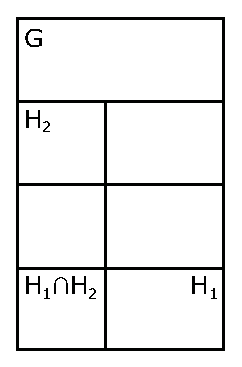
\includegraphics[width=100pt]{resources/figures/1_coset.eps}
		\caption{A illustrative figure to show $[G:H_1]>[H_2:H_1\cap H_2]$.}
		\label{fig:coset} 
	\end{figure}
	
	\begin{definition}
		We define a\textbf{ normal subgroup} $H$ of $G$ to be a subgroup such that
	\begin{equation}
		\forall g\in G:g^{-1}Hg=H
	\end{equation}
	\end{definition}
	
\begin{lemma}
	A left coset relative to a normal subgroup is a right coset.
\end{lemma}
	
	\begin{theorem}
		Cosets relative to a normal subgroup $H$ of group $G$ form a group under set product, and the unit element is $[e]=H$. This group is called the \textbf{quotient group}, denotes as $G/H$.
	\end{theorem}
	\begin{proof}
		If $[g]$ and $[g']$ are cosets relative to a normal subgroup $H$
	\begin{equation}
		[g]\cdot[g']=gHg'H=(gg'g'^{-1}H)g'H=gg'(g'^{-1}Hg')H=gg'HH=gg'H=[gg']
	\end{equation}
	\end{proof}
	
	\begin{theorem}
		Let $G$ be a group and $H$ be a subgroup of index 2. Then $H$ is a normal subgroup. $\forall g\in G:g^2\in H$.
	\end{theorem}
	\begin{proof}
		If $G=H\cup gH$, $\forall h\in H: ghg^{-1}\in H$.
	\end{proof}
	
	\begin{theorem}
		Let $H$ be a normal subgroup of $G$. Let $\pi:G\rightarrow G/H$ be $h\rightarrow [h]_H$. Then $K\rightarrow \pi(K)$ is a 1-1 correspondence between the subgroups of $G$ that contains $H$ to subgroups of $G/H$. If $K'$ is a normal subgroup of $G/H$, then $\pi^{-1}(K')$ is a normal subgroup of $G$.
	\end{theorem}
	\begin{proof}
		Let $K$ be a subgroup of $G$ that contains $H$. Clearly $\pi^{-1}(\pi(K))=K$. So $\pi$ is injective. Let $K$ be a subgroup of $G/H$. It's easy to see that $\pi^{-1}(K)$ is a subgroup of $G$ that contains $H$. So $\pi$ is surjective. So $\pi$ is a 1-1 correspondence. Let $K'$ be a normal subgroup of $G/H$. $\forall g\in G: g\pi^{-1}(K')g^{-1}=\pi^{-1}(\pi(g\pi^{-1}(K')g^{-1}))=\pi^{-1}([g]_HK'[g]_H^{-1}))=\pi^{-1}(K')$. So $\pi^{-1}(K')$ is a normal subgroup of $G$.
	\end{proof}
	
	\paragraph{Note}
		Cosets and quotient groups can be defined in another way:
		
		Let $\sim$ be an equivalent relation in monoid $M$. Define $\sim$ to be a congruence iff it satisfies that $a\sim b \wedge c \sim d \Rightarrow ab\sim cd$. This ensures the composition $[a]\cdot[b]=[ab]$ well-defined. Let $[M]=\{[m]|m\in M\}$. Then $([M],\cdot,[1])$ forms a monoid.
		
		If $M$ is a group, $([M],\cdot,[1])$ is also a group. Then $[1]$ is a normal subgroup of $M$ and $[a]$s are cosets of $[1]$. $([M],\cdot,[1])$ is just the quotient group $M/[1]$.
		
\begin{definition}
	Let $H$ and $T$ be  subgroups of group $G$. We define an equivalence relation in $G$ as
	\begin{equation}
		g_1\sim g_2 \iff \exists h\in H, t\in T: g_1=hg_2 t
	\end{equation}
	
	Each equivalent classes are called \textbf{ ($H,T$)-double cosets}, denoted by $[G]_{H,T}$. The coset containing $g$ is denoted by $[g]_{H,T}$.
\end{definition}
	\section{Some Concepts}
	
	\begin{definition}
	The \textbf{center} of a group is the set of elements that commutes with every elements in $G$, denoted by $Z(G)$. That is
	\begin{equation}
		Z(G)=\{x\in G|\forall g\in G:gx=xg\}
	\end{equation} 
	\end{definition}
	
	\begin{definition}
	The \textbf{centralizer} of a set $H$ in group $G$ is the set of elements that commutes with every elements in $H$, denoted by $C_G(H)$. That is
	\begin{equation}
		C_G(H)=\{x\in G|\forall g\in H:gx=xg\}
	\end{equation} 
	\end{definition}
	
	\begin{definition}
	The \textbf{normalizer} of a set $H$ in group $G$, denoted by $N_G(H)$, is defined by
	\begin{equation}
		N_G(H)=\{z\in G|zH=Hz\}
	\end{equation} 
	\end{definition}
	
	Normally  we abbreviate $C_G(\{x\})$ for $C_G(x)$
	\begin{lemma}
		$Z(G)$ is a normal subgroup of $G$, and $C_G(H)$ and $N_G(H)$ is a subgroup of $G$.
	\end{lemma}
	
	\section{Commutator}
	
	\begin{definition}
		Let $G$ be a group. The {\bf commutator} of $g_1,g_2\in G$ is $[g_1,g_2]=g_1g_2g_1^{-1}g_2^{-1}$.
	\end{definition}
	
	\begin{definition}
		Let $G$ be a group. The {\bf commutator subgroup} of $G$ is $\langle\{[g_1,g_2]|g_1,g_2\in G\}\rangle$.
	\end{definition}

	\begin{lemma}
		Let $G$ be a group, and $H$ be the commutator subgroup of $G$. Then $H$ is a normal subgroup.
	\end{lemma}
	\begin{proof}
		Let $S=\{[g_1,g_2]|g_1,g_2\in G\}$. Since $t[g_1,g_2]t^{-1}=[tg_1t^{-1},tg_2t^{-1}]$, it's easy to see that $N_G(S)=G$. Then $N_G(H)=G$.
	\end{proof}
	\begin{lemma}
		Let $G$ be a group, and $H$ be the commutator subgroup of $G$. Then $G/H$ is abelian.
	\end{lemma}
	\begin{proof}
		$[a]\cdot[b]\cdot[a^{-1}]\cdot[b^{-1}]=[aba^{-1}b^{-1}]=1$.
	\end{proof}
	
	\begin{lemma}
		Let $G$ be a group, $H$ be the commutator subgroup of $G$, and $K$ is a normal subgroup of $G$. $G/K$ is abelian iff $H\subseteq K$.
	\end{lemma}
	\begin{proof}
		$G/K$ is abelian $\Leftrightarrow \forall a,b: [aba^{-1}b^{-1}]_K=1\Leftrightarrow \forall a,b:aba^{-1}b^{-1}\in K\Leftrightarrow H\subseteq K$.
	\end{proof}
	
\section{Homomorphism and Isomorphism}
\begin{definition}
	Let $G_1$ and $G_2$ be two groups. We define a map $f$ from $G_1$ to $G_2$ to be a {\bf homomorphism} if
	\begin{equation}
	\forall g,h\in G_1:f(g)\circ f(h)=f(g\circ h)
	\end{equation}
	and $f(e)=e$.
\end{definition}
	\begin{lemma}
		Let $f$ be a homomorphism. $f(g)^{-1}=f(g^{-1})$
	\end{lemma}
\begin{definition}
	A homomorphism is called a(n)
	\begin{enumerate}
		\item {\bf monomorphism} if it's injective
		\item {\bf epimorphism} if it's surjective
		\item {\bf isomorphism} if it's bijective, denoted by $\cong$
	\end{enumerate}
\end{definition}
	
\begin{definition}
	A homomorphism from $G$ to itself is called an {\bf endomorphism}. An isomorphism from $G$ to itself is called an {\bf automorphism}.
\end{definition}
	
\begin{lemma}
	All automorphisms of $G$ form a group under function composition. This is called $Aut(G)$.
\end{lemma}	
	
\begin{definition}
	Let $f$ be a homomorphism from $G_1$ to $G_2$, its {\bf kernel} is defined as $\ker(f)=f^{-1}(e)$ while its {\bf image} is defined as ${\rm im}(f)=f(G_1)$.
\end{definition}
\begin{lemma}
	$\ker(f)$ is a normal subgroup of $G_1$ and ${\rm im} (f)$ is a subgroup of $G_2$. $G_1/\ker(f)\cong{\rm im}(f)$.
\end{lemma}
\begin{definition}
	Let $G$ be a group. We define the group of {\bf inner automorphisms} $Inn(G)$ to be the collection of maps $I_a$, defined by $I_a(x)=axa^{-1}$.
\end{definition}	
		
\begin{lemma}
	The map $I:G\mapsto Inn(G)$ defined by $I(a)=I_a$ is a homomorphism with kernel $C(G)$. Thus $Inn(G)\cong G/C(G)$. 
\end{lemma}
		
\begin{lemma}
	$Inn(G)$ is a normal subgroup of $Aut(G)$. 
\end{lemma}
\begin{proof}
	$f^{-1}(af(x)a^{-1})=f^{-1}(a)x(f^{-1}(a))^{-1}$
\end{proof}
		
\begin{definition}
	$Aut(G)/Inn(G)$ is called the group of {\bf outer automorphisms}.
\end{definition}

\begin{lemma}
	Let $H$ be a subset of $G$. Let $I$ be the homomorphism $N_G(H)\mapsto Aut(H)$ by $I(g)(h)=ghg^{-1}$. Then the kernel of $I$ is $C_G(H)$.
\end{lemma}
\begin{definition}
	Let $G_1$ and $G_2$ be two groups. We define a map $f$ from $G_1$ to $G_2$ to be an {\bf anti-homomorphism} if
	\begin{equation}
		\forall g,h\in G_1:f(g)\circ f(h)=f(h\circ g)
	\end{equation}
	and $f(e)=e$.
\end{definition}
	
\begin{lemma}
	If $f$ is a homomorphism, $g\mapsto f(g)^{-1}$ is an \textbf{anti-homomorphism}
\end{lemma}
\begin{definition}
	An \textbf{anti-isomorphism} is an anti-homomorphism that is bijective.
\end{definition}
	
	
\section{Isomorphism Theorems}
	\begin{theorem}
		Let $K$ be a normal subgroup of $H$, which is a subgroup of $G$. Then $H/K$ is a subgroup of $G/K$. Let $f$ be a map from the subgroups of $G$ that contains $H$ to the subgroups of $G/K$, defined by $f(T)=T/K$. Then $f$ is bijective.
	\end{theorem}
	
	\begin{theorem}
		Let $K$ be a normal subgroup of $H$, which is a subgroup of $G$. Then $H/K$ is a normal subgroup iff $H$ is a normal subgroup of $G$. In this case, $G/H\cong (G/K)/(H/K)$.
	\end{theorem}
	\begin{proof}
		Obviously $H/K$ is a subgroup of $G/K$. Then it's a normal subgroup iff
		\begin{equation}
			[g]_K(H/K)[g]_K^{-1}=\{[g]_K[h]_K[g^{-1}]_K|h\in H\}=\{[ghg^{-1}]_K|h\in H\}=H/K
		\end{equation}
		
		It's easy to prove that this is equivalent to
		\begin{equation}
			gHg^{-1}=H
		\end{equation}
		
		Finally we give an isomorphism map
		\begin{equation}
			f([g]_H)=[[g]_K]_{H/K}
		\end{equation}
		
	\end{proof}
	\begin{theorem}
		Let $H$ and $K$ be subgroups of $G$, $K$ normal in $G$. Prove that $HK$ is a subgroup of $G$ containing $K$ as normal subgroup, $H\cap K$ is normal in $H$, and $HK/K\cong H/(H\cap K)$.\
	\end{theorem}
	\begin{proof}
		The proof is straightforward. the isomorphism map is 
		\begin{equation}
			f([hk]_K)=[h]_{H\cap K}
		\end{equation}
	\end{proof}

\section{Direct product and Semi-direct Product}
\begin{definition}
	The {\bf direct product} of two groups $G_1$ and $G_2$ is a group denoted as $G_1\times G_2$, with the set $G_1\times G_2$ (treated as Cartesian product of sets), and multiplication rule as
	\begin{equation}
		(g_1,g_2)\circ(g_1',g_2')=(g_1\circ g_1',g_2\circ g_2')
	\end{equation}
\end{definition}
\begin{definition}
	The {\bf semi-direct product} of two groups $G_1$ and $G_2$ is a group denoted as $G_1\rtimes G_2$, with the set $G_1\times G_2$ and multiplication rule as
	\begin{equation}
		(g_1,g_2)\circ(g_1',g_2')=(g_1\circ \phi_{g_2}(g_1'),g_2\circ g_2')
	\end{equation}
	where $\phi_{g}$ is a homomorphism from $G_2$ to ${\rm Aut}(G_1)$.
\end{definition}
\begin{lemma}
	Let $H$ be a normal subgroup of $G$, and for each $[g]$. Suppose there exist a homomorphism $f$ from $G/H$ to $G$ such that $f([g])\in[g]$ for every $[g]\in G/H$.
	
	We define the multiplication rule of semi-direct product group $H\rtimes G/H$ as
	\begin{equation}
		(h,[g])\circ(h',[g]')=(h\circ f([g])\circ h'\circ f([g])^{-1},[g]\circ [g]')
	\end{equation}
	The map $g$ from $H\rtimes G/H$ to $G$ defined by
		\begin{equation}
			g(h,[g])=h\circ f([g])
		\end{equation}
		is an isomorphism.
\end{lemma}
	In general, we have the theorem
	\begin{theorem}[Schur,Zassenhaus]
		Let $H$ be a normal subgroup of a finite group $G$. If $|H|$ and $|G/H|$ are relatively prime, then $G\cong H\rtimes G/H$ for some $\phi$.
	\end{theorem}
	
	\section{Group acting on sets}
\begin{definition}
	All bijective maps from a set $X$ to itself form a group under map composition, this is called the \textbf{permutation group} of X, denoted by $S_X$. The unit element is just the identity map. Any subgroup of this group is called a \textbf{group of transformation} (on $X$).
\end{definition}
\begin{theorem}[Cayley]
	 Any group is isomorphic to a group of transformation
\end{theorem}
\begin{proof}
	The isomorphism from $G$ to group of transformation on $G$ is just $g\rightarrow f_g$ where $f_g$ is a map defined as $f_gg'=g\circ g'$.
\end{proof}
	
\begin{definition}
	An {\bf action} of a group $G$ on $X$ is a triple $(G,X,P)$, where $P$ a homomorphism $G\mapsto S_X$. We usually use $\circ$ for the map $P$, writing $P(g)(x)$ as $g\circ x$. With an action $(G,X,\circ)$, we also call $X$ a {\bf $G$-set}.
\end{definition}

\begin{definition}
	We say the action of $G$ on $X$ is {\bf faithful} if the homomorphism $G\mapsto S_X$ is injective.
\end{definition}
	
\begin{definition}
	If we define the equivalent relation over $X$ as
	\begin{equation}
		X\sim Y \iff\exists g:g\circ x=y
	\end{equation}
		
	The equivalent classes are called \textbf{orbits}, denoted by $O_i$, where $i$ is the index to distinguish different orbits. The action is called \textbf{transitive} if there is only one orbit. 
	
	Obviously, if $|X|$ is finite, $|X|=\sum_i|O_i|$.
\end{definition}
	
\begin{definition}
	For a point $x\in O_i$, the elements $g$ of $G$ such that $g\circ x=x$ is called the \textbf{stabilizer} of $x$, denoted by $S_x$.
\end{definition}
	\begin{lemma}
		$S_x$ is a subgroup of $G$.
	\end{lemma}
	\begin{lemma}
		If $h\circ x=y$, then $S_y=h\circ S_x \circ h^{-1}$. Thus if $x,y\in O_i$, $|S_x|=|S_y|$.
	\end{lemma}
	
\begin{lemma}
	There is a 1-1 map between $G/S_x$ and $O_i$ defined by
	\begin{equation}
		f([g])=g\circ x
	\end{equation}
\end{lemma}
	
\begin{corollary}
	If $|G|$ is finite, we have the \textbf{counting formula}: $|G/S_x|=|O_i|$ and $|G|=|O_i||S_x|$.
\end{corollary}


\begin{example}
	We define the {\bf conjugation action} of a group $G$ on itself as $g\circ g'=gg'g^{-1}$. The orbits are called conjugacy class, and two elements in an orbit are called conjugate to each other.

Let $g$ be an element of $G$. If $g\in Z(G)$, it forms a conjugacy class itself. If $g\not\in Z(G)$, its stabilizer is $C(g)$. Let $\{C_i\}$ be the conjugacy classes of $G$. Then the counting formula becomes the {\bf class equation}:
\begin{equation}
	|G|=|C(G)|+\sum_{|C_i|>1}|C_i|=|Z(G)|+\sum_{|C_i|>1}|G/C(x_i)|
\end{equation}
where $x_i\in C_i$.
\end{example}

\begin{definition}
	Let $X$ and $Y$ be $G$-sets. A map $f:X\mapsto Y$ is a {\bf homomorphism} if $\forall g\in G,x\in X:g\circ f(x)=f(g\circ x)$. If $f$ is bijective, then it's called an {\bf isomorphism}.
\end{definition}
	
\begin{example}
	Let $H$ be a subgroup of $G$. $G$ acts on $[G]_H$ by $g\circ[a]_H=[ga]_H$.
\end{example}
	
\begin{lemma}
	Let $(G,X,\circ)$ be a transitive action and $x\in X$. There's a $G$-set isomorphism $f:X\mapsto [G]_{S_x}$ defined by $f(g\circ x)=[g]_{S_x}$ .
\end{lemma}

\begin{definition}
	Let $X$ be a transitive $G$-set. The {\bf rank} of $X$ is the number of $S_x$-orbits of $X$.
\end{definition}

\begin{lemma}
	Let $X$ be a transitive $G$-set and $x\in X$. The rank of $X$ is the number of $(S_x,S_x)$-double cosets in $G$.
\end{lemma}
\begin{proof}
	The isomorphism $f:X\mapsto [G]_{S_x}$ induce the 1-1 map between the $S_x$-orbits and the $(S_x,S_x)$-double cosets.
\end{proof}
	
\section{Examples}
\begin{example}
	\textbf{Cyclic group} $C_n$ is the group with set $\{e,a,a^2,\dots,a^{n-1}\}$, where $a^n=e$. It describes the discreet rotation in a plane. $C_n$ is an abelian group.
\end{example}
	
\begin{example}
	\textbf{Dihedral group} $D_n$ is the group with set $\{e,a,a^2,\dots,a^{n-1},b,ab,a^2b,\dots,a^{n-1}b\}$, where $a^n=b^2=e$ and $ba=a^{-1}b$. It describes the discreet rotation in a plane together with mirror reflection. $D_n$ is a non-abelian group when $n\geq 2$.
\end{example}
	
\begin{example}
	Integers form a group under addition, called $\mathbb Z$.
\end{example}
	
\begin{example}
	$\{0,\dots,n-1\}$ form a group under addition mod $n$, called $\mathbb Z_n$. $\mathbb Z_n$ is isomorphic to $C_n$.
\end{example}
	
\begin{example}
	$\mathbb Z_2$ is isomorphic to the group defined by the set $\{-1,1\}$ under number multiplication. Sometimes we also call this group the \textbf{group of parity}.
\end{example}
	
\begin{example}
	Units of quaternion $\{\pm1,\pm i,\pm j,\pm k\}$ form a group, called the \textbf{quaternion group}. This is a non-Abelian group. The multiplication rule is
	\begin{equation}
		i^2=j^2=k^2=-1,\ ij=-ji=k,\ jk=-kj=i,\ ki=-ik=j
	\end{equation}
\end{example}
	
\begin{example}
	The $N\times N$ invertible matrices over a field $\mathbb F$ form a group under matrix multiplication. This is called \textbf{general linear group}, denoted by $GL(N,\mathbb F)$. All elements in $GL(N,\mathbb F)$ of determinate $1$ form a group called \textbf{special linear group}, denoted by $SL(N,\mathbb F)$.
\end{example}
	
\begin{example}
	Let $H$ be an $N\times N$ matrix over $\mathbb F$, and $f$ be an anti-isomorphism from $GL(N,\mathbb F)$ to itself. All matrices $T$ of $GL(N,\mathbb F)$ such that
	\begin{equation}
		f(T)HT=H
	\end{equation}
	form a group.
\end{example}

\begin{definition}
	A group is called {\bf simple} if it has no non-void proper normal subgroup.
\end{definition}
	
\begin{example}
	All finite simple groups have been classified by mathematicians into four categories:
	\begin{enumerate}
		\item Cyclic group of prime order
		\item Alternating group of degree $\geq5$
		\item Simple group of Lie type
		\item The 26 sporadic simple groups
	\end{enumerate}
\end{example}
	
\section{Permutation Group}
	
	As have defined, the permutation group of a set $X$ is all bijective maps from $X$ to itself under map composition.
	\begin{lemma}
		If $|X|=N$ is finite, the permutation group of $X$ is isomorphic to the permutation group of $\{1,2,\dots,N\}$.
	\end{lemma}
	
	So in order to study the general permutation group, we only need to study $S_N$.
	
\begin{definition}
	For an element $f$ of $S_N$, we may express $f$ as 
	\begin{equation}
		\left(\begin{array}{ccccc}
		1&2&3&\cdots&N\\
		f(1)&f(2)&f(3)&\cdots&f(N)
		\end{array}\right)
	\end{equation}
	Note that we don't require elements in the first row to be of ascending order.
\end{definition}
	
\begin{lemma}
	\begin{equation}
		\left(\begin{array}{cccc}
		1&2&\cdots&N\\
		f(1)&f(2)&\cdots&f(N)
		\end{array}\right)\circ
		\left(\begin{array}{cccc}
		1&2&\cdots&N\\
		g(1)&g(2)&\cdots&g(N)
		\end{array}\right)=\left(\begin{array}{cccc}
		1&2&\cdots&N\\
		f(g(1))&f(g(2))&\cdots&f(g(N))
		\end{array}\right)
	\end{equation}
	\begin{equation}
		\left(\begin{array}{cccc}
		1&2&\cdots&N\\
		f(1)&f(2)&\cdots&f(N)
		\end{array}\right)^{-1}=
		\left(\begin{array}{cccc}
		1&2&\cdots&N\\
		f^{-1}(1)&f^{-1}(2)&\cdots&f^{-1}(N)
		\end{array}\right)=\left(\begin{array}{cccc}
		f(1)&f(2)&\cdots&f(N)\\
		1&2&\cdots&N
		\end{array}\right)
	\end{equation}
\end{lemma}
\subsection{Cycle Decomposition}
\begin{definition}
	An element of the type
	\begin{equation}
		\left(\begin{array}{ccccccc}
		i_1&i_2&\cdots&i_m&a&b&\cdots\\
		i_2&i_3&\cdots&i_1&a&b&\cdots
		\end{array}\right)
	\end{equation}
	is called an \textbf{m-cycle}, denoted by $C=(i_1,i_2,\dots,i_m)$. It's length is defined as $|C|=m$. A cycle of length 2 is called a \textbf{transposition}.
\end{definition}
	\begin{lemma}
		$(i_1,\dots,i_n)=(i_1,i_n)\circ\cdots\circ(i_1,i_2)$.
	\end{lemma}
	
\begin{definition}
	We say two cycles $(i_1,\dots,i_m)$ and $(j_1,\dots,j_t)$ are disjoint if $\{i_1,\dots,i_m\}$ and $\{j_1,\dots,j_t\}$ are disjoint.
\end{definition}
	\begin{lemma}
		Two disjoint cycles commutes.
	\end{lemma}
	
	\begin{lemma}
		Each $f\in S_N$ is a product of disjoint cycles. The product is unique for each element if the omit the difference on the order of the production.
	\end{lemma}
	\begin{proof}
	For each $f\in S_N$, let $\{O_i\}$ be the orbits of $\langle f\rangle$. If $|O_i|=m$ and $a\in O_i$. Then $O_i=\{f^n(a)|n=0,\dots,m-1\}$ and $f^{(m)}(a)=a$. We define a cycle for each $O_i$ as $C_i=(a,f(a),\dots,f^{(m-1)}(a))$. $C_i$s are mutually disjoint, and $f=\prod_iC_i$.
	\end{proof}
	
	\begin{definition}
		For $g\in S_N$, we have cycle decomposition $g=C_1\cdots C_p$, rearranged so that $|C_1|<\dots<|C_p|$.  Then we define $(|C_1|,\dots,|C_p|)$ as the cycle type of $g$.
	\end{definition}
	
	\begin{theorem}
		The conjugacy class of $S_N$ are elements of the same cycle type.
	\end{theorem}
	
\subsection{Sign Function}
\begin{definition}
	Let $f$ be a permutation on $\{1,\dots,N\}$ with cycle type $(|C_1|,\dots,|C_p|)$. We define the {\bf sign} of $f$ as 
	\begin{equation}
		{\rm sgn}(f)=\prod_i (-1)^{|C_i|+1}=(-1)^{N+p}
	\end{equation}
	
	Especially ${\rm sgn}(e)=1$.
\end{definition}
\begin{lemma}
	${\rm sgn}((ab)\circ g)=-{\rm sgn}(g)$
\end{lemma}
	\begin{proof}
		\begin{eqnarray}
			(ab)(a,c_1,\dots,c_n,b,d_1,\dots,d_m)&=&(a,c_1,\dots,c_n)(b,d_1,\dots,d_m)\\
			(ab)(a,c_1,\dots,c_n)(b,d_1,\dots,d_m)&=&(a,c_1,\dots,c_n,b,d_1,\dots,d_m)
		\end{eqnarray}
	\end{proof}
	
	\begin{lemma}
		Each element of $S_N$ can be decomposed into product of transpositions.
	\end{lemma}
	\begin{proof}
		Each element can be decomposed into cycles and each cycles can be decomposed into transpositions.
	\end{proof}
\begin{lemma}
	Suppose we can write $f$ as
	\begin{equation}
		f=\prod_{i=1}^mS_i
	\end{equation}
	where $S_i$ are transpositions. 
	
	Then ${\rm sgn}(f)=(-1)^m$. This means that each element can only be decomposed into a product of even number of transpositions if is sign is 1, and odd if $-1$.
\end{lemma}
\begin{proof}
	\begin{equation}
		\prod_{i=m}^1S_if=e
	\end{equation}
	
	Then
	\begin{equation}
		{\rm sgn}\Big(\prod_{i=m}^1S_if\Big)=(-1)^m{\rm sgn}(f)=1
	\end{equation}
\end{proof}
	\begin{lemma}
		sgn is a homomorphism from $S_N$ to $\mathbb Z_2$.
	\end{lemma}
	\begin{proof}
		To prove ${\rm sgn}(f\circ g)={\rm sgn}(f)\cdot{\rm sgn}(g)$, decompose $f$ into product of transpositions.
	\end{proof}
	
\section{Alternating Group}
\begin{definition}
	The kernel of sgn forms a subgroup of $S_N$, called the \textbf{alternating group}, denoted by $A_N$.
\end{definition}
	
	\begin{theorem}
		Let $g\in A_N\subseteq S_N$. $g\in C_A$ is a conjugacy class of $A_N$, and $g\in C_S$ is a conjugacy class of $S_N$. It's easy to see that $C_A\subseteq C_S\subseteq A_N$ and $C_{A_N}(g)=C_{S_N}(g)\cap A_N$. If $C_{S_N}(g)\subseteq A_N$, then $|C_A|=|C_S|/2$. Otherwise, $|C_A|=|C_S|$.
	\end{theorem}
	\begin{proof}
		\begin{equation}
			[C_{S_N}(g):C_{A_N}(g)]=\frac{|C_{S_N}(g)|}{|C_{A_N}(g)|}=\frac{|S_N|/|C_S|}{|A_N|/|C_A|}=2|C_A|/|C_S|= 1\ {\rm or}\ 2
		\end{equation}
		
		\begin{equation}
			|C_A|=|C_S|/2\Leftrightarrow[C_{S_N}(g):C_{A_N}(g)]=1\Leftrightarrow C_{S_N}(g)=C_{A_N}(g)\Leftrightarrow C_{S_N}(g)\subseteq A_N
		\end{equation}
	\end{proof}
	
	\begin{theorem}
		Let $g\in A_N\subseteq S_N$. We have $C_{S_N}(g)\subseteq A_N$ iff the cycle decomposition of $g$ contains cycles of distinct odd length.
	\end{theorem}
	\begin{proof}
		Let $g=\prod_i c_i$ is the cycle decomposition. If $\exists c_i$ of even length, then $c_i\in C_{S_N}(g)-A_N$. If $\exists c_i,c_j$ of same odd length. Let $c_i=(a_1,\dots,a_n)$ and $c_j=(b_1,\dots,b_n)$. Then $(a_1 b_1)\cdots(a_n,b_n)\in C_{S_N}(g)-A_N$. If $\{c_i\}$ are cycles of distinct odd length. Then $h\in C_{S_N}(g)\Rightarrow h=\prod_i c_i^{n_i}\Rightarrow h\in A_N$.
	\end{proof}
	
	\begin{theorem}
		Let $C$ be a conjugacy class of $S_N$ and $C\in A_N$. If the cycle decomposition of $C$ contains cycles of distinct odd length, then $C$ splits into two conjugacy class of $A_N$ of the same size. Otherwise, $C$ is a conjugacy class of $A_N$.
		\label{thm:conj_an}
	\end{theorem}
	
	\begin{lemma}
		Each element of $A_N$ can be decomposed into product of 3-cycles.
	\end{lemma}
	\begin{proof}
		$(a,b)=(1,a)(1,b)(1,a)$ and $(1,a)(1,b)=(1,b,a)$.
	\end{proof}
\subsection{Simplicity of $A_n$}

\begin{lemma}
	$A_4$ is not simple
\end{lemma}
\begin{proof}
	A normal subgroup is $\{(1,2)(3,4),(1,3)(2,4),(1,4)(2,3),(1)(2)(3)(4)\}$.
\end{proof}

\begin{lemma}
	$A_5$ is simple.
\end{lemma}
\begin{proof}
	The conjugacy classes of $A_5$ are: $(5)$ with 12 elements, $(5)$ with 12 elements, $(3,1,1)$ with 20 elements, $(2,2,1)$ with 15 elements and $(1,1,1,1,1)$ with 1 element.
	
	Any normal subgroup of $A_5$ must be a union if conjugacy classes.
\end{proof}

\begin{lemma}
	Let $H$ be a normal subgroup of $A_n(n\geq 5)$. If $H$ contains a 3-cycle, then $H=A_n$.
\end{lemma}
\begin{proof}
	Any two 3-cycles are conjugated in $A_n(n\geq 5)$, since the cycle decomposition of a 3-cycle is $(1,\dots,1,3)$.
\end{proof}

\begin{lemma}
	Let $H$ be a normal subgroup of $G$, and $K$ be a simple subgroup of $G$. Then $K\subseteq H$ or $H\cap K= 1$.
\end{lemma}
\begin{proof}
	$H\cap K$ is a normal subgroup of $K$.
\end{proof}

\begin{lemma}
	$A_n(n\geq 5)$ is simple.
\end{lemma}
\begin{proof}
	Suppose $n>5$. Let $H$ be a nontrival normal subgroup of $A_n$. Let $\alpha\in H$ be an element that move $i$ to $j$. Let $\beta$ be a 3-cycle that fixes $i$ and moves $j$. It's easy to see that $\alpha\beta\neq\beta\alpha$. Let $a=\beta\alpha\beta^{-1}\alpha^{-1}$. Clearly $a=(\beta\alpha\beta^{-1})\alpha^{-1}\in H$, and $a=\beta(\alpha\beta^{-1}\alpha^{-1})$ is a product of 2 3-cycles. So $a$ moves at most 6 elements.
	
	If $a$ moves 6 elements (in this case $n\geq 6$), $a$ has the cycle type $(3,3,1,\dots)$. Since elements with cycle type $(3,3,1,\dots)$ form a unique conjugacy class, $(123)(456)$ and $(654)(123)\in H$. So $(132)\in H$. So $H=A_n$.
	
	Otherwise $a$ moves at most 5 elements. Let $A_5$ be the subgroup of $A_n$ that moves these 5 elements. Then $H\cap A_5\neq 1$. So $A_5\subseteq H$. So $H$ contains a 3-cycle. So $H=A_n$.
\end{proof}
	
	\section{Sylow's Theorems}
	
	\begin{definition}
		Let $p$ be a prime number. By a {\bf p-group}, we mean a group of order $p^n$.
		
		Let $G$ be a finite group. We call a subgroup of $G$ that is a $p$-group a {\bf p-subgroup}.
		
		Let $H$ be a $p$-subgroup of $G$ and $|H|=p^m$. We call $H$ {\bf p-Sylow subgroup} if $p^m$ is the highest power of $p$ that divides $|G|$.
	\end{definition}
	
	\begin{lemma}
		Let $G$ be a finite abelian group, and let $p$ be a prime number dividing $|G|$. Then $G$ has an element of order $p$.
	\end{lemma}
	\begin{proof}
		We prove this by induction on $|G|$. The lemma certainly holds for $|G|=1$.
		
		When $|G|>1$, we choose $g\in G$ of order $m>1$. If $p|m$, then $g^{m/p}$ is of order $p$. If $p\not| m$, $p\big ||G/(g)|$. Since $|G/(g)|<|G|$, we have an element $(h)\in G/(g)$ of order $p$. Let $h\in G$ be of order $n$. Then $(h)^n=(1)$. So $p|n$. Then $h^{n/p}$ is of order $p$.
	\end{proof}
	
	\begin{theorem}[Sylow I]
		If $p$ is a prime number and $p^k\big||G|$. Then $G$ contains a subgroup of order $p^k$.
	\end{theorem}
	\begin{proof}
		We prove this by induction on $|G|$. The theorem certainly holds for $|G|=1$.
		
		When $|G|>1$, we have the class equation
		\begin{equation}
			|G|=|Z(G)|+\sum_i[G:C(x_i)]
		\end{equation}
		
		If $p\not\big||Z(G)|$, $\exists i:p\not|[G:C(x_i)]$. So $p^k|C(x_i)$ and $|C(x_i)|<|G|$. So $C(x_i)$ contains a subgroup of order $p^k$. If $p\big||Z(G)|$, from the lemma, $\exists g\in Z(G)$ of order $p$. So $p^{k-1}\big||G/(g)|$. Since $|G/(g)|<|G|$ and $(g)$ is normal, $\exists H/(g)$ of order $p^{k-1}$, and $H$ is of order $p^k$.
	\end{proof}
	
	\begin{lemma}
		Let $P$ be a Sylow $p$-subgroup of $G$, and $H$ a subgroup of order $p^k$ contained in $N_G(P)$. Then $H\subseteq P$.
		\label{lem:sylow_pgroup}
	\end{lemma}
	\begin{proof}
		Since $P$ is normal subgroup of $N_G(P)$, $HP$ is a subgroup of $G$ and $HP/P\simeq H/(H\cap P)$. So $|HP/P|=|H/(H\cap P)|=p^s$. So $|HP|=p^s|P|$. Since $P$ is a Sylow $p$-subgroup, $|HP|=|P|$. So $HP=P$. So $H\subseteq P$.
	\end{proof}
	
	\begin{lemma}
		Let $H$ be a $p$-group acting on a finite set $S$. Then the number of fixed points of $H\equiv |S| \mod p$.
		\label{lem:sylow_mod1}
	\end{lemma}
	
	\begin{theorem}[Sylow II]
		\begin{enumerate}
			\item Any two Sylow $p$-subgroups of $G$ are conjugate in $G$
			\item The number of Sylow $p$-subgroups divides the index of any Sylow p-subgroups, and $\equiv 1\mod p$.
			\item Any $p$-subgroup is contained in a Sylow p-subgroup.
		\end{enumerate}
	\end{theorem}
	\begin{proof}
		Let $\Pi$ be the set of all Sylow $p$-subgroups. For each $p$-subgroup $P\in \Pi$, $P$ acts on $\Pi$ by conjugation. Let $P'$ be a fixed point of the action. Then $P\subseteq N_G(P')\Rightarrow P=P'$. So $P$ is the only fixed point. Let $O$ be an orbit in $\Pi$. From (\ref{lem:sylow_mod1}), $|O|\equiv 1 \mod p$ if $P\in O$, and $|O|\equiv 0 \mod p$ if $P\not\in O$. Since this holds for any $P\in\Pi$, $\Pi$ is the only orbit. So $|\Pi|\equiv 1 \mod p$. Since $G$ acts transively on $|\Pi|$ by conjugation, we have $|\Pi|=[G:N_G(P)]$. So $|\Pi|\big| [G:P]$.
		
		Let $H$ be a $p$-subgroup of order $p^k (k>0)$. $H$ acts on $\Pi$ by conjugation. Since $|\Pi|\equiv 1 \mod p$, $H$-action has at least one fixed point, say $P_0$. Then $H\subseteq N_G(P_0)$. So by the lemma (\ref{lem:sylow_pgroup}), $H\subseteq P_0$.
	\end{proof}
	
	\begin{corollary}
		Let $G$ be a group and $N$ a normal subgroup of $G$. If $P$ is a Sylow p-subgroup of $N$ then $G=N_G(P)N$.
	\end{corollary}
	\begin{proof}
		$\forall g\in G$, $gPg^{-1}$ is a Sylow p-subgroup of $N$. So by Sylow II, $\exists n\in N$ such that $gPg^{-1}=nPn^{-1}$. So $g^{-1}n\in N_G(P)$.
	\end{proof}

	\section{Solvability and Nilpotenty}
	
	\begin{definition}
		Let $G$ be a finite group. $G$ is said to be {\bf solvable} if there exist a series $\{G_0,\dots,G_n\}$ of normal subgroups of $G$ such that 
		\begin{equation}
			1=G_0\triangleleft G_1\triangleleft\cdots\triangleleft G_n= G
		\end{equation}
		and $G_{i+1}/G_i$ is abelian.
	\end{definition}
	
	\begin{theorem}
		Let $H$ be a normal subgroup of $G$. $G$ is solvable iff $H$ and $G/H$ are solvable.
	\end{theorem}
	
	\begin{theorem}
		Let $p$ be a prime number. $p$-group is solvable.
	\end{theorem}
	
	\begin{proof}
		Let $G$ be a $p$-group of order $p^k(k>1)$. We prove by induction on $k$. If $k=1$, $G$ is cyclic and thus solvable. If $k>1$, we have class equation
		\begin{equation}
			|G|=|Z(G)|+\sum_i[G:C(x_i)]
		\end{equation}
		Clearly $p\big||Z(G)|$. So $C(G)$ is non-trivial. If $Z(G)=G$, clearly $G$ is solvable. Otherwise $Z(G)$ is a normal subgroup of $G$ and by induction $Z(G)$ and $G/Z(G)$ are solvable. So $G$ is solvable.
	\end{proof}
	
	\begin{theorem}
		Let $p$ and $q$ be distinct prime numbers. A group of order $pq$ is solvable.
	\end{theorem}
	\begin{proof}
		Let $G$ be a group of order $pq$. Let's assume $p<q$. Let $N_q$ be number of $q$-Sylow subgroups. By Sylow theorem, we have $N_q|p$ and $N_q \equiv 1 \mod q$. So $N_q=1$. So there's only one $q$-Sylow subgroup and it's normal and solvable. Let it be $H$. $G/H$ is cyclic and thus solvable. So $G$ is solvable.
	\end{proof}
	
	\begin{definition}
		Let $G$ be a finite group. $G$ is said to be {\bf nilpotent} if there exist a series $\{G_0,\dots,G_n\}$ of normal subgroups of $G$ such that 
		\begin{equation}
			1=G_0\triangleleft G_1\triangleleft\cdots\triangleleft G_n= G
		\end{equation}
		and $G_{i+1}/G_i=Z(G/G_i)$.  
	\end{definition}
	
	\begin{theorem}
		A nilpotent group is solvable.
	\end{theorem}
	
\chapter{Mathieu Groups}

\section{Block System}
	
\begin{definition}
	Let $G$ be a group that acts on a set $S$ transitively. A {\bf block system} is a partition $\Pi$ of $S$ such that $\forall B\in \Pi\forall g\in G:gB\in \Pi$. Each $B\in S$ is called a {\bf block} if it's in some block system.
\end{definition}

A block system is a coarse-grained action.

\begin{lemma}
	Let $G$ be a group that acts on a set $S$ transitively. Let $\Pi$ be a block system of $S$. For each $B\in \Pi$, $\Pi=\{gB|g\in G\}$. So $\Pi$ is uniquely determined by one of its element.
\end{lemma}

\begin{lemma}
	Let $G$ be a group that acts on a set $S$ transitively. $B\subseteq S$ is a block if $\forall g\in G: gB=B\vee gB\cap B=\emptyset$.
\end{lemma}

\begin{lemma}
	Non-empty intersection of blocks is a block.
\end{lemma}

\begin{definition}
	Let $G$ be a group that acts on $X$ transitively. Let $\Pi$ be a block system of $S$. For each $B\in \Pi$, the {\bf stabilizer} of $B$ is defined as $S_B=\{g\in G|gB=B\}$. Clearly $x\in B\Rightarrow S_x$ is a subgroup of $S_B$.
\end{definition}

There's an isomorphism between the action on the left cosets and the action on the block system.

\begin{definition}
	A transitive action is called {\bf primitive} iff it contains no non-trivial block system
\end{definition}
\begin{definition}
	Let $G$ be a group that acts on $X$ transitively. The action is called {\bf maximal} iff each $S_x$ is maximal.
\end{definition}

\begin{lemma}
	Let $G$ be a group that acts on a set $X$ transitively. For each $x\in X$, there's 1-1 correspondence between non-trivial subgroup containing $S_x$ ($H$ such that $G\supsetneq H\supsetneq S_x$) and a non-trivial block containing $x$ (a block that's not $\{x\}$ or $S$).
\end{lemma}
\begin{proof}
	For each $H$ such that $G\supsetneq H\supsetneq S_x$, we define $f(H)$ by $\{Hx\}$. It's easy to see that $f$ is injective. For each non-trivial block $B\ni x$, let $H_B=\{g\in G|gx\in B\}$. It's easy to see that $H_B$ is a non-trivial subgroup containing $S_x$ and $f(H_B)=B$. So $f$ is surjective.
\end{proof}

\begin{corollary}
	Let $(G,X,\circ)$ be a transitive action. The action is primitive iff it's maximal.
\end{corollary}

\begin{lemma}
	Let $(G,X,\circ)$ be a primitive action. Let $H\neq 1$ be a normal subgroup of $G$. Then $H$ acts transitively on $X$.
\end{lemma}
\begin{proof}
	For each $x$, $Hx=HS_xx=Gx=X$.
\end{proof}

\section{Multiple transitivity}

\begin{definition}
	Let $(G,S,\circ)$ be an action. Let $\Delta(S^n)=\{(s_1,\dots,s_n)|s_i\in S, s_1\neq\cdots\neq s_n\}$. We have a natural action $(G,\Delta(S^n),\circ)$ defined by $g\circ(s_1,\cdots,s_n)=(g\circ s_1,\cdots,g\circ s_n)$. The action $(G,S,\circ)$ is called {\bf n-transitive} if the action $(G,\Delta(S^n),\circ)$ is transitive.
\end{definition}

\begin{lemma}
	Let $(G,S,\circ)$ be an action. If the action is k-transitive, then the action is n-transitive for any $n\leq k$.
\end{lemma}

\begin{lemma}
	Let $(G,S,\circ)$ be an action. Then the action is k-transitive iff $S_x$ acts on $(X-\{x\})$ $(k-1)$-transitively for each $x\in X$.
\end{lemma}

\begin{lemma}
	A 2-transitive action is primitive.
\end{lemma}
\begin{proof}
	There's no non-trivial block.
\end{proof}

\begin{definition}
	Let $(G,S,\circ)$ be an action. $(G,S,\circ)$ is called {\bf sharply n-transitive} if the action $(G,\Delta(S^n),\circ)$ satisfied that $\forall(s_1,\dots,s_n)\in \Delta(S^n): S_{(s_1,\dots,s_n)}=1$. 
\end{definition}

\begin{lemma}
	Let $(G,S,\circ)$ be an action. Then the action is sharply k-transitive iff $S_x$ acts on $(X-\{x\})$ sharply $(k-1)$-transitively for each $x\in X$.
\end{lemma}

\begin{lemma}
	$S_n$ acts sharply n-transitively on $\{1,\dots,n\}$ for every $n$. $A_n$ acts sharply $(n-2)$-transitively on $\{1,\dots,n\}$ for every $n\geq 3$.
\end{lemma}

\begin{definition}
	A sharply 1-transitive action is called {\bf regular}.
\end{definition}

\begin{lemma}
	A sharply n-transitively is faithful.
\end{lemma}


\section{Affine Geometry}

\begin{definition}
	A set $A$ is an $n$-dimensional {\bf affine space} if there's a map $\rightarrow:A\times A\mapsto K^n$ (n-dimension linear space over the field $K$) such that 
	\begin{enumerate}
		\item For each $x\in A$, the partial map $y\mapsto\overrightarrow{xy}$ is a bijection from $A$ to $ K^n$.
		\item For each $x,y,z\in A$, $\overrightarrow{xy}+\overrightarrow{yz}=\overrightarrow{xz}$.
	\end{enumerate}
\end{definition}

\begin{definition}
	Let $V$ be an $n$-dimensional linear space. For each $m$-dimensional subspace $S\subseteq V$ and each $v\in V$, $S+v$ is called an $m$-dimensional {\bf affine subspace} of $V$. A 0-dimensional affine subspace is called a {\bf point}. A 1-dimensional affine subspace is called a {\bf line}. An $(n-1)$-dimensional affine subspace is called a {\bf hypersurface}.
\end{definition}
Clearly an $m$-dimensional affine subspace of $V$ is an affine space by defining $\overrightarrow{xy}=y-x$.

\begin{definition}
	Let $U$ and $V$ be n-dimensional linear spaces. A bijective map $f:U\mapsto V$ is an {\bf affine isomorphism} iff $\forall S\subseteq U,f(S)$ an affine subspace of $V\Leftrightarrow S$ is an affine subspace of $U$. The affine automorphisms of $V$ is denoted by $Aut(V)$.
\end{definition}

\begin{definition}
	Let $U$ be a linear space. The {\bf affine group} $Aff(U)$ is defined to be the transformations on $U$
	\begin{equation}
		u\mapsto g\cdot u+a
	\end{equation}
	for all $g\in GL(U)$ and $a\in U$.
\end{definition}

\begin{lemma}
	$Aff(U)\subseteq Aut(U)$
\end{lemma}

\begin{definition}
	Let $V$ and $V'$ be vector spaces over $K$. A function $f:V\mapsto V'$ is a {\bf semilinear transformation} if there's $\sigma\in Aut(K)$ such that $\forall x,y\in V,\forall\lambda\in K$
	\begin{eqnarray}
		f(x+y)&=&f(x)+f(y)\\
		f(\lambda x)&=&\sigma(\lambda)x
	\end{eqnarray}
	A semilinear transformation is nonsingular if it is a bijection. All non-singular semilinear transformations on a linear space $V$ form a group denoted by $\Gamma L(V)$.
\end{definition}

\begin{lemma}
	$\Gamma L(V)\subseteq Aut(U)$
\end{lemma}

\begin{lemma}
	Let $V$ be a linear space of dimension $\geq 2$ over a field $K$. Then
\end{lemma}


	
	\chapter{Linear Representation of Finite Group}
	
	\begin{definition}
		
	A \textbf{linear representation} of a group $G$ is a homomorphism $T$ from $G$ to general linear group of $V$. For our purpose, we require $V$ to be  a finite dimensional complex linear space.
	\end{definition}
	
	\begin{example}
	Obviously $T(g)=id$ is a representation, called the \textbf{identity representation}.
	\end{example}

	
	\begin{definition}
	Two linear representations are said \textbf{equivalent} if they are related by a similar transformation, that is 
	\begin{equation}
		T_1\sim T_2\iff T_1=ST_2S^{-1}
	\end{equation}
	\end{definition}
	
	\begin{lemma}
		Each linear representations is a unitary representations relative to some inner product.
	\end{lemma}
	\begin{proof}
	From an arbitrary inner product $H_0$ on $V$, we can define a new inner product
	\begin{equation}
		H(u,v)=\sum_{g\in G}H_0(T(g)u,T(g)v)
	\end{equation}
	
	It's easy to see that $H$ is an inner product and $\forall g \in G: H(u,v)=H(T(g)u,T(g)v)$.
	
	Thus $T(g)$s are isometries with respect to $H$, and thus unitary. This means we can always find an inner product such that $T(g)$s are unitary. 
	\end{proof}
	We'll use this inner product from now on.
	\section{Reducibility}
	
	\begin{definition}
	A set of operators $T_i:V\mapsto V$ is said to be {\bf reducible} if it has a non-trival proper invariant subspace of $V$. That is
	\begin{equation}
		\exists 0\neq V_0\subsetneq V\ \forall i:T_iV_0\subset V_0
	\end{equation}
	\end{definition}

	
	\begin{lemma}
		Let $T$ be a non-singular operator. Then $T V_0\subset V_0\iff T V_0=V_0$.
	\end{lemma}
	
	\begin{definition}
	A set of unitary operators $T_i$ is called {\bf completely reducible} if we can divide $V$ into $V_1\oplus V_2$ such that
	\begin{equation}
	\forall i:T_iV_1\subset V_1\wedge T_iV_2\subset V_2
	\end{equation}
	
	From the lemma above, that means
	\begin{equation}
	\forall i:T_iV_1=V_1\wedge T_iV_2=V_2
	\end{equation}
	
	\end{definition}
	\begin{theorem}
		If a set of unitary operators is reducible, then it is completely reducible.
	\end{theorem}
	\begin{proof}
		If $T_i$ is reducible with a proper invariant subspace $V_0$, then
		\begin{equation}
		V=V_0\oplus V_0^\bot
		\end{equation}
		
		Since $T_i$ is an isometry,
		\begin{equation}
		\forall i:T_iV_0^\bot\bot T_iV_0=V_0
		\end{equation}
		
		Thus for all $i$, $T_iV_0^\bot\subset V_0^\bot$, and thus $T_iV_0^\bot= V_0^\bot$.
		
		Thus $T_i$ is completely reducible.
	\end{proof}
	
	\begin{definition}
	A representation of a group $G$ is (completely) reducible iff the set $\{T(g)|g\in G\}$ is (completely) reducible.
	\end{definition}
	
	\begin{lemma}
		A representation of a group $G$ is completely reducible if its reducible.
	\end{lemma}
	
	For a set of unitary operators $T_i$ on $V$. If $T_i$ is reducible, we can reduce it into $V=V_1\oplus V_2$. Then we consider $T_i|_{V_1}$ and $T_i|_{V_2}$. If $T_i|_{V_1}$ is reducible, we can reduce it into $V_1=V_{1,1}\oplus V_{1,2}$ \dots We continue this procedure until we decompose $V$ into $V_1\oplus\cdots\oplus V_n$ such that $T_i|_{V_j}$ is irreducible. This is called the reduction of a set of unitary operators. As we have shown, we can choose $V_1$ \dots $V_n$ so they are mutually orthogonal. (This can be strictly proved by induction on the dimension of $V$)
	
	\begin{lemma}
		If $T(g)$ is irreducible, then so is $T^\dagger(g)$. 
	\end{lemma}
	\begin{proof}
		 $T^\dagger(g)$ is also unitary. If it's reducible, then it's completely reducible, which leads to the reducibility of $T(g)$.
	\end{proof}
	\section{Schur's Lemma}
	\begin{lemma}[Schur]
		If $T(g)$ is an irreducible representation of group $G$ over linear space $V$. $P$ is any linear transformation over $V$ and
		\begin{equation}
			\forall g:T(g)P=PT(g)
		\end{equation}
		then $P=\lambda I$.
	\end{lemma}
	\begin{proof}
		Define $P_\lambda=P-\lambda I$. Since $\det P_\lambda=\det(P-\lambda I)$ always has a root in $\mathbb C$, we can choose $\lambda$ so that $P_\lambda$ is singular.
		
		Obviously we also have
		\begin{equation}
			\forall g:T(g)P_\lambda=P_\lambda T(g)
		\end{equation}
		
		Thus
		\begin{equation}
		\forall g:T(g)P_\lambda V=P_\lambda T(g)V=P_\lambda V
		\end{equation}
		
		Thus $P_\lambda V$ is an invariant subspace.
		
		Since $T(g)$ is irreducible, $P_\lambda V=V$ or $\emptyset$.
		
		Since $P_\lambda$ is singular, $P_\lambda V=\emptyset$. Thus $P_\lambda=0$, $P=\lambda I$
	\end{proof}
	\begin{corollary}
		Abelian groups only have 1-D irreducible representations.
	\end{corollary}
	\begin{lemma}[Schur]
		If $T(g)$ and $T'(g)$ are two inequivalent irreducible representations of group $G$ over linear space $V$ and $V'$. $P$ is any linear transformation from $V'$ to $V$ and
		\begin{equation}
			\forall g:T(g)P=PT'(g)
		\end{equation}
		then $P=0$.
	\end{lemma}
	\begin{proof}
		Choose any inner products over $V$ and $V'$. Assume $P\neq0$, thus $P^\dagger\neq0$.
		\begin{equation}
		\forall g:T(g)P V'=P T'(g)V'=PV'
		\end{equation}
		
		And
		\begin{equation}
		\forall g:P^\dagger T^\dagger(g)=T'^\dagger(g)P^\dagger
		\end{equation}
		thus
		\begin{equation}
		\forall g:T'^\dagger(g)P^\dagger V=P^\dagger T^\dagger(g) V=P^\dagger V
		\end{equation}
		
		Since $T(g)$ and $T'^\dagger(g)$ are both irreducible, if $P\neq 0$, $P V'=V$ and $P^\dagger V=V'$.
		
		This means that $P$ is invertible, thus
		\begin{equation}
			\forall g:P^{-1}T(g)P=T'(g)
		\end{equation}
		and $T(g)$ and $T'(g)$ are equivalent. This is a contradiction.
		
		Thus $P=0$.
	\end{proof}
	\begin{theorem}[Wigner,Eckart]
	If $D(g)$ is a unitary group representation over a complex linear space.
	
	We have an orthonormal basis $|a,j,x\rangle$ such that
	\begin{equation}
		\langle a,j,x|D(g)|b,k,y\rangle=\delta_{ab}\delta_{xy}[D^a(g)]_{jk}
	\end{equation}
	where $a$ labels different irreducible representations, $j$ labels the representation indices, and $x$ labels equivalent representations. 
	
	If D is a symmetry for the operator O, that is 
	\begin{equation}
		D(g)OD(g)^\dagger=O\Rightarrow[O,D(g)]=0
	\end{equation}
	
	Then
	\begin{equation}
		\langle a,j,x|O|b,k,y\rangle=O(a)_{xy}\delta_{ab}\delta_{jk}
	\end{equation}
	\end{theorem}	
	
	\begin{proof}
		
	\begin{eqnarray}
		0&=&\langle a,j,x|[O,D(g)]|b,k,y\rangle\\
		&=&\langle a,j,x|O|c,l,z\rangle\langle c,l,z|D(g)|b,k,y\rangle-\langle a,j,x|D(g)|c,l,z\rangle\langle c,l,z|O|b,k,y\rangle\\
		&=&\langle a,j,x|O|b,l,y\rangle[D^a(g)]_{lk}-[D^a(g)]_{jl}\langle a,l,x|O|b,k,y\rangle
	\end{eqnarray}
	
	Use Schur's lemma.
	\end{proof}
	
	When considering the set of all inequivalent irreducible representations, we use a superscript to distinguish among them, such as $T^a$
	
	\begin{lemma}
		In matrix form, we have the \textbf{orthogonality relation}
	\begin{eqnarray}
		\frac 1{|G|}\sum_gT^{a\dagger}_{si}(g)\delta_{il}\delta_{jm}T^b_{jt}(g)&=&\frac{\delta_{lm}}{d_a}\delta_{ab}\delta_{st}\\
		\frac {d_a}{|G|}\sum_gT^{a*}_{ls}(g)T^b_{mt}(g)&=&\delta_{ab}\delta_{lm}\delta_{st}\label{eqn:orthogonal}
	\end{eqnarray}
	\end{lemma}
	\begin{proof}
	For two irreducible representations $T^a$ and $T^b$ and any map $D$ from $V^b$ to $V^a$, since
	\begin{eqnarray}
		\big(\sum_gT^{a\dagger}(g)DT^b(g)\big)T^b(g')&=&\sum_gT^{a\dagger}(g)DT^b(g\circ g')\\
		&=&\sum_gT^{a\dagger}(g\circ g'^{-1})DT^b(g)\\
		&=&T^a(g')\sum_gT^{a\dagger}(g)DT^b(g)
	\end{eqnarray}
	
	From Schur's lemma, we have 
	\begin{equation}
		\frac 1{|G|}\sum_gT^{a\dagger}(g)DT^b(g)=\lambda\delta_{ab}I
	\end{equation}	
	
	By taking trace on both sides, we know if $a=b$, $\lambda=\frac{{\rm Tr}[D]}{d_a}$, where $d_a$ is the dimension of $T^a$.
	
	In matrix form, choose $D_{ij}$ to be $\delta_{il}\delta_{jm}$. We have the orthogonality relation.
	\end{proof} 	
	
	\section{Regular Representation}
	\begin{definition}
		We define the {\bf group space} as a vector space of $|G|$ dimension, where each basis vector corresponds to an element of $G$. That is, we can express a basis as $\vv g$.
	\end{definition}
	
	\begin{example}
		
	Then we have two natural representation of $G$ on the group space called \textbf{left/right regular representation}. The left regular representation is defined by
	\begin{equation}
		L(g')c_g\vv g=c_g\vv{g'\circ g}
	\end{equation}
	and the right regular representation is defined by
	\begin{equation}
		R(g')c_g\vv g=c_g\vv{g\circ g'^{-1}} 
	\end{equation}
	
	We define the inner product in the group space as
	\begin{equation}
	(\vv h,\vv g)=\delta_{gh}
	\end{equation}
	Both regular representations are unitary under this inner product.
	
	We define $\vv{T^a_{ij}}$ as 
	\begin{equation}
		\vv{T^a_{ij}}=\sum_gT^a_{ij}(g)\vv{g}
	\end{equation}
	
	Then
	\begin{equation}
		\big(\vv T^b_{kl},\vv{T^a_{ij}}\big)=\sum_gT^{b*}_{kl}(g)T^a_{ij}(g)=\frac{|G|}{d_a}\delta_{ab}\delta_{ik}\delta_{jl}
	\end{equation}
	
	So $\vv{T^a_{ij}}$s are orthogonal for different $(a,i,j)$.
	
	We have
	\begin{eqnarray}
		R(g)\vv{T^a_{ij}}&=&\sum_hT^a_{ij}(h)\vv{h\circ g^{-1}}\\
		&=&\sum_hT^a_{ij}(h\circ g)\vv{h}\\
		&=&T^a_{kj}(g)\vv{T^a_{ik}}
	\end{eqnarray}
	
	So that $\vv{T^a_{ij}}$s ($a$ and $i$ fixed) form an invariant subspace, in which $R(g)$ transforms like $T^a$.
	
	Similarly
	\begin{equation}
		L(g)\vv{T^a_{ij}}=T^{a\dagger}_{ik}(g)\vv{T^a_{kj}}
	\end{equation}
	
	Next we prove that $\vv{T^a_{ij}}$s are complete. 
	
	For an arbitrary vector $\vv v$, we have $\vv v=\sum \vv{v_a}$ such that each $\vv{v_a}$ is in $V_a$, an irreducible subspace of $R(g)$. Thus $R|_{V_a}$ is similar to some irreducible representation, say $T^a$. Then we can find a basis $\vv{e_i}$ on $V_i$ such that
	\begin{equation}
		R(g)\vv{e_j}=T^a_{ij}(g)\vv{e_i}
	\end{equation}
	
	We may expand $\vv{e_j} $ as $\sum_he_{jh}\vv h$ where $h\in G$, we have
	\begin{equation}
		\sum_he_{jh}\vv{h\circ g^{-1}}=\sum_hT^a_{ij}(g)e_{jh}\vv h
	\end{equation}
	
	Compare the coefficient on both sides, we have
	\begin{eqnarray}
		\forall h,g&:&e _{j(h\circ g)}=T^a_{ij}(g)e_{ih}\\
		\forall g&:&e _{jg}=T^a_{ij}(g)e_{ie}
	\end{eqnarray}
	
	Thus
	\begin{equation}
		\vv{e_j}=\sum_he_{jg}\vv g=\sum_hT^a_{ij}(g)e_{ie}\vv g=e_{ie}\vv{T^a_{ij}}
	\end{equation}
	
	Thus
	\begin{equation}
		\vv v_a=v_j\vv{e_j}=v_je_{ie}\vv{T^a_{ij}}
	\end{equation}
	
	Such each $\vv {v_a}$ can be expand by $\vv{T^a_{ij}}$s. Such each $\vv v$ can be expand by $\vv{T^a_{ij}}$s.
	
	Thus $\vv{T^a_{ij}}$s form a orthogonal complete basis. And clearly the right regular representation can be reduced into
	\begin{equation}
		R=\bigoplus_a(T^a)^{\oplus d_a}
	\end{equation}
	\end{example}
	
	Counting the dimension of both sides, we have 
	\begin{theorem}[Burnside]
		$|G|=\sum_ad_a^2$
	\end{theorem}
	
	\section{Characters}
	
	\begin{definition}
		
	\textbf{Characters} of a group representation $T$ are defined as	
	\begin{equation}
		\chi(g)={\rm Tr}[T(g)]
	\end{equation}
	\end{definition}
	
	\begin{lemma}
		If $g$ is conjugate to $g'$, then $\chi(g)=\chi(g')$. Thus $\chi(g)$ is a function of conjugate class, thus we sometime write 
	$\chi(C_i)$ where $C_i$ is the i-th conjugate class.
	\end{lemma}
	
	As before, we define $\chi^a$ for each inequivalent irreducible representation $T^a$.
	
	\begin{lemma}
		We have the orthogonality relation for characters
	\begin{equation}
		\frac 1{|G|}\sum_g\chi^{a*}(g)\chi^b(g)=\delta_{ab}
	\end{equation}	
	or
	\begin{equation}
		\sum_i|C_i|\chi^{a*}(C_i)\chi^b(C_i)=|G|\delta_{ab}
	\end{equation}	
	\end{lemma}
	\begin{proof}
		Taking traces on both sides of Eqn. \ref{eqn:orthogonal}.
	\end{proof}
	
	\begin{definition}
	We define the {\bf class space} as the subspace of group space that contains all vector $|v\rangle$ such that
	\begin{equation}
		\forall g:R(g)L(g)\vv v=\vv v
	\end{equation}
	\end{definition}
	
	\begin{lemma}
	For each character $\chi$ we define the corresponding vector in the group space as
	\begin{equation}
		\vv \chi=\chi(g)\vv g
	\end{equation}
	$\vv \chi$ is contained in the class space.
	\end{lemma}
	
	\begin{lemma}
		$\vv {\chi^a}$s for characters of irreducible representations form an orthogonal complete basis
	\end{lemma}
	\begin{proof}
	We have
	\begin{eqnarray}
		(\vv{\chi^a},\vv{\chi^b})=\sum_g\chi^{a*}(g)\chi^b(g)=|G|\delta_{ab}
	\end{eqnarray}
	
	Thus $\vv{\chi^a}$s are orthogonal to each other.
	
	For each $\vv v$ is the class space, we can expand  $\vv v$ over $\vv{T_{ij}^a}$ as
	\begin{equation}
		\vv v=\sum_av^a_{ji}\vv{T_{ij}^a}
	\end{equation}	
	
	We have
	\begin{eqnarray}
		R(g)L(g)\vv v&=&\sum_aR(g)L(g)v^a_{ji}\vv{T_{ij}^a}\\
		&=&\sum_aT_{lj}^a(g)T_{ik}^{a\dagger}(g)v^a_{ji}\vv{T_{kl}^a}\\
		&=&\vv{v}=\sum_av^a_{lk}\vv{T_{kl}^a}
	\end{eqnarray}
	
	Thus
	\begin{eqnarray}
		T_{lj}^a(g)T_{ik}^{a\dagger}(g)v^a_{ji}&=&v^a_{lk}\\
		T_{lj}^a(g)v^a_{ji}&=&T_{ki}^a(g)v^a_{lk}
	\end{eqnarray}
	
	From Schur's lemma, we have
	\begin{equation}
		v^a_{ij}=v^a\delta_{ij}
	\end{equation}
	
	Thus
	\begin{equation}
		\vv v=\sum_av^a\delta_{ij}\vv{T_{ij}^a}=\sum_av^a\vv{\chi^a}
	\end{equation}	
	
	Thus $\vv{\chi^a}$s form an orthogonal complete basis over the class space.
	\end{proof}
	
	\begin{lemma}
		If the representation $T$ can be reduced into $T^a\oplus\cdots\oplus T^z$, then its character $\chi(g)=\chi^a(g)+\cdots+\chi^z(g)$. Thus $\vv\chi=\vv{\chi^a}+\cdots+\vv{\chi^z}$. The expansion coefficients of $\vv\chi$ over $\vv{\chi^a}$s are integers and just means the recurrence of different irreducible representations where $T$ is reduced.
	\end{lemma}
	\begin{proof}
	\begin{eqnarray}
		\chi(g)&=&{\rm Tr}[T(g)]\\
		&=&{\rm Tr}\left[\left(\begin{array}{ccc}
			T^a(g)&\cdots&0\\
			\vdots&\ddots&\vdots\\
			0&\cdots&T^z(g)
		\end{array}	\right)\right]\\
		&=&{\rm Tr}[T^a(g)]+\cdots+{\rm Tr}[T^z(g)]\\
		&=&\chi^a(g)+\cdots+\chi^z(g)
	\end{eqnarray}
	\end{proof}
	
	\begin{lemma}
		
	For each conjugate class $C_i$ of $G$, we construct a vector
	\begin{equation}
		\vv{C_i}=\sum_{g\in C_i}\vv g
	\end{equation}	
	 $\vv{C_i}$s is an orthogonal complete basis of the class space.
	 \end{lemma}
	
	\begin{corollary}
		The dimension of the class space is the number of inequivalent irreducible representations, and is also the number of conjugate classes.
	\end{corollary}
	
	\begin{lemma}
		We have the second orthogonality relation
	\begin{equation}
		\sum_a|C_i|\chi^{a*}(C_i)\chi^a(C_j)=|G|\delta_{ij}\label{eqn:2nd-ortho}
	\end{equation}
	\end{lemma}
	\begin{proof}
	We define a matrix $\Gamma$ as 
	\begin{equation}
		\Gamma_{ij}=\sqrt{\frac{|C_j|}{|G|}}\chi^i(C_j)
	\end{equation}
	
	From the arguments above we know that $\Gamma$ is a square matrix. And the orthogonality relation tell us that $\Gamma\Gamma^\dagger=I$. Thus $\Gamma^\dagger\Gamma=I$.
	\end{proof}
	
	\section{Group Algebra}
	\begin{definition}
			We define the multiplication over the group space as
	\begin{equation}
		\vv x\cdot\vv y=\Big(\sum_gx_g\vv g\Big)\cdot\Big(\sum_hy_h\vv h\Big)=\sum_g\sum_hx_gy_h\vv{gh}
	\end{equation}
	
	Thus the group space forms an associative algebra called the \textbf{group algebra}.
	\end{definition}

	
	Obviously
	\begin{eqnarray}
		\vv e\cdot\vv v&=&\vv v\\
		\vv g\cdot\vv{g^{-1}}&=&\vv e\\
		L(g)\vv v&=&\vv g\cdot\vv v\\
		R(g)\vv v&=&\vv v\cdot\vv{g^{-1}}
	\end{eqnarray}
	
	\begin{lemma}
		A vector $\vv v$ belongs to the class space iff $\forall g\in G:\vv g\cdot\vv v\cdot\vv{g^{-1}}=\vv v $.
	\end{lemma}
	
	\begin{lemma}
	\begin{equation}
		\vv{C_i}\cdot\vv{C_j}=f_{ijk}\vv{C_k}
	\end{equation}
	where $f_{ijk}$ is an integer.
	\end{lemma}
	\begin{proof}
	Clearly $\vv g\cdot\vv{C_i}\cdot\vv{g^{-1}}=\vv{C_i}$.
	
	Since
	\begin{equation}
		\vv g\cdot\vv{C_i}\cdot\vv{C_j}\cdot\vv{g^{-1}}=\vv g\cdot\vv{C_i}\cdot\vv{g^{-1}}\cdot\vv g\cdot\vv{C_j}\cdot\vv{g^{-1}}=\vv{C_i}\cdot\vv{C_j}
	\end{equation}
	$\vv{C_i}\cdot\vv{C_j}$ belongs to the class space. It can be expressed as
	\begin{equation}
		\vv{C_i}\cdot\vv{C_j}=f_{ijk}\vv{C_k}
		\label{eqn:class_vec_decomp}
	\end{equation}
	
	Obviously $\vv{C_i}\cdot\vv{C_j}$ has integers coefficients expanding on $\vv g$ basis. Then clearly $f_{ijk}$ is an integer.
	\end{proof}
	

	\begin{definition}
	For each representation $T:G\mapsto GL(V)$ , we define a map $T$ from the group algebra to $hom(V)$ by
	\begin{equation}
		T(\vv v)=\sum_gv_gT(g)
	\end{equation}
	where $\vv v=v_g\vv g$.
	\end{definition}

\begin{lemma}
		The $T$ defined above is an algebra homomorphism, sometimes called the \textbf{representation of the group algebra}.
\end{lemma}
\begin{proof}
	\begin{eqnarray}
		T(\vv v)T(\vv{v'})&=&\sum_{gg'}v_gT(g)v'_{g'}T(g')\\
		&=&\sum_{gg'}v_gv'_{g'}T(gg')\\
		&=&\sum_{gg'}T(v_gv'_{g'}\vv{gg'})\\
		&=&T(\vv v\cdot\vv {v'})
	\end{eqnarray}
\end{proof}
\begin{lemma}
		$T(\vv{C_i})=\frac{|C_i|}{d}\chi(C_i) I$, where $d$ is the dimension of the representation space.
\end{lemma}
\begin{proof}
	\begin{eqnarray}
		T(g)T(\vv{C_i})T(g^{-1})&=&T(\vv g)T(\vv{C_i})T(\vv{g^{-1}})\\
		&=&T(\vv g\cdot\vv{C_i}\cdot\vv{g^{-1}})\\
		&=&T(\vv{C_i})
	\end{eqnarray}
	
	Thus $T(g)T(\vv{C_i})=T(\vv{C_i})T(g)$. From Schur's lemma, $T(\vv{C_i})=\lambda I$. By taking traces, $\lambda =\frac{|C_i|}{d}\chi(C_i)$.
\end{proof}
	
\begin{lemma}
	For a group representation $T^a$,
	\begin{equation}
		\frac{|C_i|}{d_a}\chi^a(C_i)\frac{|C_j|}{d_a}\chi^a(C_j)=f_{ijk}\frac{|C_k|}{d_a}\chi^a(C_k)\label{eqn:character}
	\end{equation}
	where $f_{ijk}$ is defined in Eqn. \ref{eqn:class_vec_decomp}.
\end{lemma}
\begin{proof}
	\begin{equation}
		T^a(\vv{C_i}\cdot\vv{C_j})=T^a(\vv{C_i})T^a(\vv{C_j})=f_{ijk}T^a(\vv{C_k})
	\end{equation}
\end{proof}
	
	\section{$d_a\big||G|$}
	\begin{definition}
		An element $a\in\mathbb F$ is an \textbf{algebraic integer} if its the root of some monic polynomials in $\mathbb F[x]$ with integral coefficient.	
	\end{definition}

	\begin{theorem}
		The set of all algebraic integers (relative to $\mathbb F$) forms a ring.
	\end{theorem}
	\begin{proof}
		If $a$ is an algebraic integer and $a^n+\sum_{i=0}^{n-1}z_ia^i=0$, clearly $\{1,\dots,a^{n-1}\}$ generates $\mathbb Z[a]$.
		
		If $a$ and $b$ are algebraic integers, $\mathbb Z[a]$ and $\mathbb Z[b]$ are finitely generated. Then clearly $\mathbb Z[a,b]$ is finitely generated. Since $\mathbb Z[a,b]$ is a Noether module, it's submodules $\mathbb Z[a+b]$ and $\mathbb Z[ab]$ are finitely generated. Suppose $\mathbb Z[a+b]$ is generated by $\{f_1(a+b),\dots,f_n(a+b)\}$ and their maximal degree is $d$. Then $(a+b)^{(d+1)}=z_if_i(a+b)$. Thus $a+b$ is an algebraic integer. Similarly $ab$ is an algebraic integer.
	\end{proof}	
	\begin{theorem}
		The algebraic integer (relative to $\mathbb C$) that is rational is an integer.
	\end{theorem}
	\begin{theorem}
		The eigenvalues of an integer matrix are algebraic integers.
	\end{theorem}
	
	\begin{theorem}
		$d_a\big||G|$
	\end{theorem}
	\begin{proof}
	Clearly, the character $\chi^a(g)$ (of irreducible representation $T^a(g)$) is the sum of some eigenvalues of $L(g)$, which is a integer matrix under the basis $|g\rangle$. Thus $\chi^a(g)$ is an algebraic integer.
	
	Equation (\ref{eqn:character}) can be viewed as an eigenvalue equation of the matrix $(f_i)_{jk}$. Thus the eigenvalue $\frac{|C_i|}{d_a}\chi^a(C_i)$ is an algebraic integer.
	
	Obviously the complex conjugation of an algebraic integer is an algebraic integer.
	
	From (\ref{eqn:2nd-ortho}) we have
	\begin{equation}
	\sum_a\frac{|C_i|}{d_a}\chi^{a*}(C_i)\chi^a(C_i)=\frac{|G|}{d_a}
	\end{equation}
	
	The LHS is an algebraic integer, thus $\frac{|G|}{d_a}$ is also an algebraic integer. But $\frac{|G|}{d_a}$ is rational. So it is an integer.	
	\end{proof}
	
	\section{Character Table}
	The characters of irreducible representations have many advantages over the representations themselves. Firstly the characters are very concise. Secondly they're fixed while the representations can vary by a similar transformation. Thirdly, they provide us much information to reduce an arbitrary representation.
	
	Thus for groups, people usually list $\chi^a(C_i)$s of all inequivalent irreducible representations $a$ over all conjugacy classes $C_i$ in the form a \textbf{character tables}, such as Tab. \ref{tab:character_table}.
	\begin{table}[htb!]
		\centering
		\begin{tabular}{|c|c|c|c|}
			\hline
			&$C_1$&$\cdots$&$C_n$\\
			\hline
			$\chi^1$&$\chi^1(C_1)$&$\cdots$&$\chi^1(C_n)$\\
			\hline
			$\cdots$&$\cdots$&$\ddots$&$\cdots$\\
			\hline
			$\chi^n$&$\chi^n(C_1)$&$\cdots$&$\chi^n(C_n)$\\
			\hline
		\end{tabular}
		\caption{A character table.}
		\label{tab:character_table}
	\end{table}
	
	For most situations, the character table is uniquely determined by the equations for the characters that we have derived, which includes
	\begin{enumerate}
		\item The number of the inequivalent irreducible representations is the number of conjugacy classes.
		\item The Burnside theorem $|G|=\sum_ad_a^2$.
		\item $d_a\big||G|$
		\item The orthogonality relations:
		\begin{eqnarray}
			\sum_i|C_i|\chi^{a*}(C_i)\chi^b(C_i)&=&|G|\delta_{ab}\label{eqn:orth1}\\
			\sum_a|C_i|\chi^{a*}(C_i)\chi^a(C_j)&=&|G|\delta_{ij}\label{eqn:orth2}
		\end{eqnarray}	
		\item
		\begin{equation}
			\frac{|C_i|}{d_a}\chi^a(C_i)\frac{|C_j|}{d_a}\chi^a(C_j)=f_{ijk}\frac{|C_k|}{d_a}\chi^a(C_k)
		\end{equation}
	\end{enumerate}
	
	Note that for the identity representation, we can fill in $\chi(C_i)=1$ without hesitation. We also have $\chi^a(e)=d_a$. We may take these to results into (\ref{eqn:orth1}) and (\ref{eqn:orth2}) and get for non-identity irreducible representation
	\begin{equation}
		\sum_i|C_i|\chi^a(C_i)=0
	\end{equation}
	and for $C_i\neq\{e\}$
	\begin{equation}
		\sum_ad_a\chi^a(C_i)=0
	\end{equation}
	
	We may also make use of the fact that for 1-D representations $T^a$, $\chi^a=T^a$.
	\section{Direct Product Representations}
	\begin{definition}
	Let $T(g)$ and $T'(g)$ be two representations of group $G$ that act on $V$ and $V'$ respectively. $T''(g)=T(g)\otimes T'(g)$ is called the\textbf{ direct product representation} of $T(g)$ and $T'(g)$.
	\end{definition}

	\begin{lemma}
	The characters of $T''(g)=T(g)\otimes T'(g)$ are $\chi''(g)=\chi(g)\chi'(g)$.
	\end{lemma}
	\begin{proof}
			\begin{equation}
		\chi''(g)={\rm Tr}[T''(g)]={\rm Tr}[T(g)\otimes T'(g)]={\rm Tr}[T(g)]{\rm Tr}[ T'(g)]=\chi(g)\chi'(g)
	\end{equation}
	\end{proof}
	
	\begin{definition}
	If $T^a(g)$ and $T^b(g)$ are irreducible representations, normally $T^n(g)=T^a(g)\otimes T^b(g)$ is reducible, and can be reduced into $\bigoplus_c(T^c)^{\oplus n_{abc}}$, which is called the\textbf{ Clebsch-Gordan series}. $n_{abc}$ is can be calculated by
	\begin{equation}
		n_{abc}=\frac 1{|G|}\langle \chi^c|\chi^n\rangle
	\end{equation}
	where $\chi^n(g)=\chi^a(g)\chi^b(g)$.	
	\end{definition}
	
\chapter{Ring}

\section{Basics}

\begin{definition}
	A {\bf ring} $(R,\cdot,+)$ is a set $R$ together with binary operators $\cdot$ and $+$ such that
	\begin{enumerate}
		\item $(R,+)$ is a abelian group with unit $0$, called the {\bf additive group}.
		\item $(R,\cdot)$ is a monoid with unit $1$, called the {\bf multiplicative monoid}.
		\item $a(b+c)=ab+ac$ and $(a+b)c=ac+bc$ hold $\forall a,b,c\in R$.
	\end{enumerate}
\end{definition}

\begin{definition}
	Let $(R,\cdot,+)$ be a ring. We define its {\bf opposite ring} $(R,\times,+)$, denoted by $R^{op}$, to be the ring with the same underlying set and addition operation, and a new multiplication defined by $a\times b=b\cdot a$.
\end{definition}
	
\begin{definition}
	Let $(R,\cdot,+)$ be a ring, $(S,\cdot,+)$ is a {\bf subring} of $(R,\cdot,+)$ if $(S,+)$ is a subgroup of $(R,+)$, and $(S,\cdot)$ is a submonoid of $(R,\cdot)$.
\end{definition}

\begin{example}
	$\mathbb Z$, $\mathbb Q$, $\mathbb R$ and $\mathbb C$ with the usual addition and multiplication are rings.
\end{example}

\begin{example}
	$\{m+n\sqrt a|m,n\in\mathbb Z\}(a\in\mathbb Z)$ is a subring of $\mathbb C$ called the {\bf Gaussian integers}.
\end{example}

\begin{definition}
	A ring $(R,\cdot,+)$ is a {\bf commutative ring} if $(R,\cdot)$ is a commutative monoid.
\end{definition}

\begin{definition}
	A commutative ring $(R,\cdot,+)$ is an {\bf integral domain} if $(R-0,\cdot)$ is a submonoid of $(R,\cdot)$.
\end{definition}

\begin{definition}
	Let $R$ be a ring. $a\in R$ is a {\bf left (right) zero divisor} if $\exists b\in R: ab=0(ba=0)$.
\end{definition}

\begin{lemma}
	A commutative ring $(R,\cdot,+)$ is an integral domain iff there's no non-zero zero divisors.
\end{lemma}
\begin{lemma}
	A commutative ring $(R,\cdot,+)$ is an integral domain iff the cancellation law holds: $ab=ac\wedge a\neq 0\Rightarrow b=c$.
\end{lemma}

\begin{definition}
	A ring $(R,\cdot,+)$ is a {\bf division ring} if $(R-0,\cdot)$ is a subgroup of $(R,\cdot)$.
\end{definition}

\begin{lemma}
	A finite integral domain is a division ring.
\end{lemma}

\begin{definition}
	A commutative division ring is called a {\bf field}.
\end{definition}

\begin{definition}
	Let $(R,\cdot,+)$ be a ring. The invertible elements of the monoid $(R,\cdot)$ are called the {\bf units} of $R$, which form a group $R^\times$.
\end{definition}

\begin{lemma}
	In a ring $R$, if $1-ab$ is invertible, then so is $1-ba$.
\end{lemma}
\begin{proof}
	$(1-ba)^{-1}=1+b(1-ab)^{-1}a$.
\end{proof}

\begin{lemma}[Hua]
	In a ring $R$, if $a,b$ and $ab-1$ is invertible, then so is $a-b^{-1}$ and $(a-b^{-1})^{-1}-a^{-1}$.
\end{lemma}
\begin{proof}
	$(a-b^{-1})^{-1}=b(ab-1)^{-1}$, $((a-b^{-1})^{-1}-a^{-1})^{-1}=aba-a$.
\end{proof}

\begin{example}
	$n\times n$ matrices with entries in a ring $K$ form a ring $M_n(K)$ under matrix addition and matrix multiplication.
\end{example}

\begin{lemma}
	Let $R$ be a commutative ring. A matrix $A\in M_n(R)$ is invertible iff its determinant is invertible in $R$.
\end{lemma}
\begin{proof}
	$adj(A)\cdot A=A \cdot adj(A)=det(A)$
\end{proof}

\begin{example}
	The {\bf quaternions} $\mathbb H$ is a subring of $M_2(\mathbb C)$ defined by $\{\begin{pmatrix}
		a&b\\-\bar b&\bar a
	\end{pmatrix}|a,b\in\mathbb C\}$.
\end{example}

\begin{lemma}
	$\mathbb H$ is a division ring.
\end{lemma}
\begin{proof}
	$det \begin{pmatrix}
		a&b\\-\bar b&\bar a
	\end{pmatrix}=|a|^2+|b|^2$.
\end{proof}

\begin{lemma}
	$\mathbb H$ is a real linear space with basis $1=\begin{pmatrix}1&0\\0&1\end{pmatrix}, i=\begin{pmatrix}i&0\\0&-i\end{pmatrix}, j=\begin{pmatrix}0&1\\-1&0\end{pmatrix}$ and $k=\begin{pmatrix}0&i\\i&0\end{pmatrix}$.
\end{lemma}

\section{Centralizer}

\begin{definition}
	The \textbf{center} of a ring is the set of elements that commutes with every elements in $R$, denoted by $Z(R)$. That is
	\begin{equation}
		Z(R)=\{x\in R|\forall r\in R:rx=xr\}
	\end{equation} 
\end{definition}

\begin{definition}
	The \textbf{centralizer} of a set $S$ in group $R$ is the set of elements that commutes with every elements in $S$, denoted by $C_R(S)$. That is
	\begin{equation}
		C_R(S)=\{x\in R|\forall s\in S:sx=xs\}
	\end{equation} 
\end{definition}

\begin{lemma}
	Let $S$ be a subset of a ring $R$ then $C_R(S)$ is a subring of $R$.
\end{lemma}

\begin{lemma}
	In a division ring, if $ab\neq ba$, we have the identity
	\begin{equation}
		a=(b^{-1}-(a-1)^{-1}b^{-1}(a-1))(a^{-1}b^{-1}a-(a-1)^{-1}b^{-1}(a-1))^{-1}
	\end{equation}
\end{lemma}

\begin{theorem}[Cartan,Brauer,Hua]
	A division ring (but not a field) $K$ is generated by a non-central element and its conjugates.
\end{theorem}
\begin{proof}
	Let $L$ be the set of all conjugates of a non-central element. Let $K'$ be the subdivision-ring generated by $L$. It's easy to see that $K'$ is normal. For each $a\in R$, if there exist $b\in K'$ not commutes with $a$, then $a=(b^{-1}-(a-1)^{-1}b^{-1}(a-1))(a^{-1}b^{-1}a-(a-1)^{-1}b^{-1}(a-1))^{-1}\in K'$. So $K-K'$ and $K'$ are commutative elementwise.
	
	If $K\neq K'$, let $a\in K-K'$ and $b,b'\in K'$ such that $bb'\neq b'b$. $b$ and $b'$ exist since otherwise $K'$ is in the center of $K$. It's easy to see that $ab\in K-K'$. Thus $(ab)b'=b'(ab)=ab'b$. Thus $bb'=b'b$, a contradiction.
\end{proof}

\begin{corollary}
	Every proper normal subdivision-ring of a division ring is contained in its center.
\end{corollary}

\section{Ideals}

\begin{definition}
	Let $R$ be a ring. A subset $I\subseteq R$ is a {\bf (two-sided) ideal} if $I$ is an additive subgroup of $R$ and $\forall g\in G:gI=Ig\subseteq I$.
\end{definition}

\begin{lemma}
	The intersection of ideals is an ideal.
\end{lemma}

\begin{definition}
	Let $R$ be a ring and $S\subseteq R$. The ideal {\bf generated by} $S$, denoted by $\langle S\rangle$, is the intersection of all the ideals that contain $S$.
\end{definition}

\begin{lemma}
	Let $R$ be a ring and $S\subseteq R$. The ideal generated by $S$ is $\{\sum_{i=0}^nl_is_ir_i|n\in \mathbb N, l_i,r_i\in R, s_i\in S\}$
\end{lemma}

\begin{definition}
	A {\bf principle ideal} is an ideal generated by one element.
\end{definition}

\begin{definition}
	An integral domain is a {\bf principle integral domain (PID)} if every ideal is principle.
\end{definition}

\begin{example}
	$\mathbb Z$ is a PID.
\end{example}

\begin{definition}
	In a commutative ring, a {\bf prime ideal} $I$ is an ideal such that $ab\in I\Rightarrow a\in I\vee b\in I$.
\end{definition}

\begin{definition}
	A {\bf maximal ideal} $I$ is an ideal of $R$ such that there's no ideal $M$ that satisfies $R\supsetneq M\supsetneq I$.
\end{definition}

\begin{lemma}
	In a commutative ring, a maximal ideal is a prime ideal.
\end{lemma}

\begin{proof}
	Let $I$ be a maximal ideal of $R$ such that $I$ is not prime. Then there're $a,b$ such that $ab\in I$, $a,b\not\in I$. Then $\langle a,I\rangle=\langle b,I\rangle=R$. Then $\exists s\in R,t\in R,x\in I,y\in T$ such that $as+x=bt+y=1$. Then $abst+(xbt+yas+xy)=1$. Then $\langle ab,I\rangle=R$, a contradiction.
\end{proof}

\begin{lemma}
	In a PID, a prime ideal is a maximal ideal.
\end{lemma}

\section{Quotient Ring}

\begin{definition}
	Let $R$ be a ring with an ideal $I$. The additive quotient group $R/I$ is a ring with the multiplication $[a]\cdot [b]=[ab]$, called the {\bf quotient ring}.
\end{definition}

\begin{example}
	$(m)=m\mathbb Z$ is an ideal in the ring $\mathbb Z$. We define the quotient ring $\mathbb Z_m=\mathbb Z/(m)$.
\end{example}

\begin{lemma}
	If $p$ is a prime number, $\mathbb Z_p$ is a field, also denoted by $F_p$.
\end{lemma}

\begin{lemma}
	Let $R$ be a ring with an ideal $I$. $I$ is prime iff $R/I$ is an integral domain.
\end{lemma}

\begin{lemma}
	Let $R$ be a ring with an ideal $I$. $I$ is maximal iff $R/I$ is a field.
\end{lemma}

	
\section{Homomorphism and Isomorphism}
\begin{definition}
	Let $R_1$ and $R_2$ be two rings. We define a map $f:R_1\mapsto R_2$ to be a {\bf homomorphism} if it's a homomorphism of both the addition group and the multiplication monoid.
\end{definition}

As with groups, we can define similar concepts of {\bf monomorphism, epimorphism, isomorphism, endomorphism, automorphism, kernel, image, inner automorphism \dots}
	
\begin{lemma}
	All automorphisms of a ring $R$ form a group under function composition. This is called $Aut(R)$.
\end{lemma}	

\begin{lemma}
	Let $f:R_1\mapsto R_2$ be a ring homomorphism. $\ker(f)$ is an ideal of $R_1$ and ${\rm im} (f)$ is a subring of $R_2$. $R_1/\ker(f)\cong{\rm im}(f)$.
\end{lemma}	

\begin{definition}
	Let $R_1$ and $R_2$ be two rings. We define a map $f:R_1\mapsto R_2$ to be a n {\bf anti-homomorphism} if it's a homomorphism of the addition group and an anti-homomorphism of the multiplication monoid.
\end{definition}

\begin{lemma}
	The composite of a homomorphism and an anti-homomorphism is an anti-homomorphism. The composite of two anti-homomorphisms is a homomorphism
\end{lemma}

\begin{lemma}
	The identity map $R\mapsto R^{op}$ is an anti-homomorphism.
\end{lemma}

\subsection{Jordan homomorphism}

\begin{definition}
	A {\bf Jordan homomorphism} $\eta: R\mapsto R'$ is an additive group homomorphism that satisfies $\eta(1)=1$ and $\eta(aba)=\eta(a)\eta(b)\eta(a)$.
\end{definition}

\begin{lemma}
	Let $\eta: R\mapsto R'$ be a Jordan homomorphism, then
	\begin{eqnarray}
		\eta(a^k)&=&\eta(a)^k, k\in \mathbb N\\
		\eta(abc+cba)&=&\eta(a)\eta(b)\eta(c)+\eta(c)\eta(b)\eta(a)\\
		\eta(ab+ba)&=&\eta(a)\eta(b)+\eta(b)\eta(a)
	\end{eqnarray}
\end{lemma}

\begin{lemma}[Hua]
	Let $\eta: R\mapsto R'$ be an additive group homomorphism that satisfies
	\begin{enumerate}
		\item $\eta(1)=1$
		\item For each $a,b\in R$, either $\eta(ab)=\eta(a)\eta(b)$ or $\eta(ab)=\eta(b)\eta(a)$
	\end{enumerate}
	Then $\eta$ is a ring homomorphism or a ring anti-homomorphism.
\end{lemma}
\begin{proof}
	For each $a\in R$, let $A_1=\{r\in R|\eta(ar)=\eta(a)\eta(r)\}$ and $A_2=\{r\in R|\eta(ar)=\eta(r)\eta(a)\}$. If $A_1\neq R$ and $A_2\neq R$, then let $r_1\in R-A_1$ and $r_2\in R-A_2$. Then $\eta(ar_1)=\eta(r_1)\eta(a)\neq\eta(a)\eta(r_1)$, and $\eta(ar_2)=\eta(a)\eta(r_2)\neq\eta(r_2)\eta(a)$. If $\eta(a(r_1+r_2))=\eta(a)\eta(r_1+r_2)$, then $\eta(r_1)\eta(a)=\eta(a)\eta(r_1)$, a contradiction. If $\eta(a(r_1+r_2))=\eta(r_1+r_2)\eta(a)$, there's a similar contradiction. So $A_1= R$ or $A_2= R$.
	
	Let $S_1=\{a\in R|\forall r\in R:\eta(ar)=\eta(a)\eta(r)\}$ and $S_2=\{a\in R|\forall r\in R:\eta(ar)=\eta(r)\eta(a)\}$. If $S_1\neq R$ and $S_2\neq R$, then let $r_1\in R-S_1$ and $r_2\in R-S_2$. Then exists $a\in R$ such that $\eta(r_1a)=\eta(a)\eta(r_1)\neq\eta(r_1)\eta(a)$. So $\eta(r_2a)=\eta(a)\eta(r_2)$, a contradiction. So $S_1= R$ or $S_2= R$. So $\eta$ is a ring homomorphism or a ring anti-homomorphism.
\end{proof}

\begin{lemma}[Jacobson, Rickart]
	Let $\eta: R\mapsto D$ be a Jordan homomorphism from a ring to a domain, then for each $a,b\in R$, either $\eta(ab)=\eta(a)\eta(b)$ or $\eta(ab)=\eta(b)\eta(a)$. Thus $\eta$ is a ring homomorphism or a ring anti-homomorphism..
\end{lemma}
\begin{proof}
	\begin{eqnarray}
		&&\eta((ab)ba+ab(ab))=\eta(ab)\eta(b)\eta(a)+\eta(a)\eta(b)\eta(ab)\nonumber\\
		&=&\eta(ab^2a+(ab)^2)=\eta(a)\eta(b)^2\eta(a)+\eta(ab)^2
	\end{eqnarray}
	So $(\eta(ab)-\eta(a)\eta(b))(\eta(ab)-\eta(b)\eta(a))=0$. So either $\eta(ab)=\eta(a)\eta(b)$ or $\eta(ab)=\eta(b)\eta(a)$.
\end{proof}

\begin{theorem}[Hua]
	Let $\eta: D\mapsto D'$ be an additive group homomorphism between division rings that satisfies
	\begin{enumerate}
		\item $\eta(1)=1$
		\item For each $0\neq a\in R$, $\eta(a)\neq 0$ and $\eta(a^{-1})=\eta(a)^{-1}$.
	\end{enumerate}
	Then $\eta$ is a ring homomorphism or a ring anti-homomorphism.
\end{theorem}
\begin{proof}
	By Hua's identity, $\eta(aba-a)=\eta(((a-b^{-1})^{-1}-a^{-1})^{-1})=((\eta(a)-\eta(b)^{-1})^{-1}-\eta(a)^{-1})^{-1}=\eta(a)\eta(b)\eta(a)-\eta(a)$. So $\eta$ is a Jordan homomorphism.
\end{proof}
	
\subsection{Isomorphism Theorems}
\begin{theorem}
	Let $K$ be an ideal contained in $I$, which is an ideal of $R$. Then $I/K$ is a ideal of $R/K$. Let $f$ be a map from the ideals of $R$ that contains $K$ to the ideals of $R/K$, defined by $f(T)=T/K$. Then $f$ is bijective. Further more, $R/I\cong (R/K)/(I/K)$.
\end{theorem}
	
\begin{theorem}
	Let $S$ be a subring of $R$, and $I$ be an ideal in $G$. Then $S+I$ is a subring of $R$ containing $I$ as an ideal, $S\cap I$ is an ideal in $S$, and $(S+I)/I\cong S/(S\cap I)$.
\end{theorem}
\begin{proof}
	The isomorphism map is 
	\begin{equation}
		f([h+k]_K)=[h]_{H\cap K}
	\end{equation}
\end{proof}

\section{Characteristic}

\begin{definition}
	Let $R$ be a ring, we have a natural homomorphism $f:\mathbb Z\mapsto R$ defined by 
	\begin{eqnarray}
		f(n)&=&\underbrace{1+\cdots+1}_n\\
		f(0)&=&0\\
		f(-n)&=&-f(n)
	\end{eqnarray}
	where $n>0$. Let $\ker f=(c)$. We define $c$ to be the {\bf characteristic} of $R$.
\end{definition}

\begin{example}
	$\mathbb Z_p$ is of characteristic $p$. $\mathbb Z$ is of characteristic 0.
\end{example}

\begin{lemma}
	The characteristic of an integral domain is a prime number.
\end{lemma}

\section{Relation of elements}

{\bf In the following sections of this chapter we assume the ring to be commutative.}

\begin{definition}
	Let $R$ be a ring and $a,b\in R$. If $\exists c:b=ac$, then $a$ {\bf divides} $b$, denoted by $a|b$. We also say that $a$ is a {\bf factor} of $b$.
\end{definition}

\begin{definition}
	Let $R$ be a ring and $a,b\in R$. If $\exists $ non-unit $ c:b=ac$, then $a$ {\bf divides properly} $b$. We also say that $a$ is a {\bf proper factor} of $b$.
\end{definition}

\begin{lemma}
	Let $R$ be a ring and $a,b\in R$. $a$ divides $b$ iff $b\in\langle a\rangle$ iff $\langle a\rangle\supseteq\langle b\rangle$.
\end{lemma}

\begin{definition}
	Let $R$ be a ring. $a\in R$ is {\bf prime} if $\forall b,c\in R:a|bc\Rightarrow a|b\vee a|c$.
\end{definition}
\begin{lemma}
	Let $R$ be a ring. $a\in R$ is prime iff $\langle a\rangle$ is a prime ideal.
\end{lemma}

\begin{definition}
	Let $R$ be a ring and $a,b\in R$. $a$ {\bf associates with} $b$, denoted by $a\sim b$, if there's a unit $u\in R$ such that $a=ub$.
\end{definition}

\begin{lemma}
	Let $R$ be a ring and $a,b\in R$. $a\sim b$, iff $\langle a\rangle=\langle b\rangle$.
\end{lemma}

\begin{definition}
	Let $R$ be a ring. $a\in R$ is {\bf irreducible} if $\forall b,c\in R:a=bc\Rightarrow b$ or $c$ is unit.
\end{definition}

\begin{lemma}
	Let $R$ be a domain. If $a\in R$ is prime, then $a$ is irreducible.
\end{lemma}

\begin{lemma}
	Let $R$ be a p.i.d. If $a\in R$ is irreducible, then $a$ is prime.
\end{lemma}

\begin{proof}
	If $a\in R$ is irreducible, then $\langle a\rangle$ is maximal.
\end{proof}

\begin{definition}
	Let $R$ be a ring and $b_i\in R$. $a\in R$ is a {\bf greatest common divisor} of $\{b_i\}$, denoted as $gcd(b_i)$, if $\forall i:a|b_i$ and for each $c\in R$ such that $\forall i:c|b_i$ we have $c|a$.
\end{definition}

\begin{lemma}
	Let $R$ be a PID and $b_i\in R$. $a=gcd(\{b_i\})$ iff $\langle a\rangle=\langle\{b_i\}\rangle$.
\end{lemma}

\begin{lemma}
	$gcd(gcd(a_1,\dots,a_n),b_1,\dots,b_n)\sim gcd(a_1,\dots,a_n,b_1,\dots,b_n)$
\end{lemma}
\begin{lemma}
	$gcd(a_1,\dots,a_n)b\sim gcd(a_1b,\dots,a_nb)$
\end{lemma}
\begin{lemma}
	If $a=gcd(a_1,\dots,a_n)$, then $\exists b_1,\dots,b_n$ such that $a=a_1b_1+\cdots a_nb_n$.
\end{lemma}

\begin{definition}
	Let $R$ be a ring and $b_i\in R$. $a\in R$ is a {\bf least common multiplier} of $\{b_i\}$, denoted as $lcm(b_i)$, if $\forall i:b_i|a$ and for each $c\in R$ such that $\forall i:b_i|c$ we have $a|c$.
\end{definition}

\begin{lemma}
	Let $R$ be a PID and $b_i\in R$. $a=lcm(\{b_i\})$ iff $\langle a\rangle=\bigcap_i\langle b_i\rangle$.
\end{lemma}


\section{Polynomial Ring}

\begin{definition}
	Let $R$ be a ring. A {\bf formal power series} over $R$ is a series $(r_i)$. The set of all formal power series form a ring $R[[x]]$, with addition and multiplication as
	\begin{enumerate}
		\item $(a_i)+(b_i)=(c_i)\Rightarrow c_i=a_i+b_i$.
		\item $(a_i)\cdot(b_i)=(c_i)\Rightarrow c_i=\sum_{j=0}^ia_j\cdot b_{i-j}$.
	\end{enumerate}
\end{definition}

\begin{definition}
	Let $R$ be a ring. The ring of {\bf polynomials} $R[x]$ is a subring of $R[[x]]$
	\begin{equation}
		R[x]=\{(r_i)\in R[[x]]|\exists n:m\geq n\rightarrow r_m=0\}
	\end{equation}
\end{definition}

There a natural embedding $\iota:R\hookrightarrow R[x]$ by defining $\iota(r)=(r,0,\cdots)$. In this way we say $R\subseteq R[x]$.

\begin{lemma}
	Let $R$ be an integral domain, $R[x]$ is also an integral domain.
\end{lemma}

\begin{lemma}
	Let $F$ be a field, $F[x]$ is a principle integral domain.
\end{lemma}

\begin{definition}
	In $R[[x]]$ we define the {\bf indeterminate} $x=(0,1,0,\cdots)$.
\end{definition}

\begin{lemma}
	$R[x]$ is generated by $R$ and $x$. $(r_i)=\sum_i r_ix^i$. So we usually denote $(r_i)$ by $u(x)$.
\end{lemma}

\begin{definition}
	Let $\sigma=(r_i)\in R[x]$ be a non-zero polynomial. The {\bf degree} of $\sigma$, denoted by $deg(\sigma)$, is $n$ such that $r_n\neq 0$ and $r_m=0$ for all $m>n$. Then we call $r_n$ the {\bf leading coefficient} of $(r_i)$. $(r_i)$ is called {\bf monic} if its leading coefficient is 1.
\end{definition}

\begin{lemma}
	Let $R$ and $S$ be rings. For each $u\in S$ and each homomorphism $\eta:R\mapsto S$, there's a unique $\eta_u:R[x]\mapsto S$ such that $\eta_u(r)=\eta(r)$ and $\eta_u(x)=u$.
\end{lemma}

\begin{definition}
	Let $R\subseteq T$ be rings. For each subset $S\subseteq T$, we define $R[S]$ to be the subring of $T$ generated by $R$ and $S$. 
\end{definition}

\begin{lemma}
	Let $R\subseteq S$ be rings, and $u\in S$. Let $i$ be the identity map on $R$. We usually write $i_u(p(x))$ as $p(u)$. It's easy to see that ${\rm im}i_u=R[u]\cong R[x]/\ker i_u$.
\end{lemma}

\begin{definition}
	Let $R\subseteq S$ be rings, and $u\in S$. Let $f(x)\in R[x]$. If $f(u)=0$, u is called a {\bf root} of $f(x)$.
\end{definition}

\begin{definition}
	Let $F$ be a field, and $R$ be a ring that contains $F$. An element $u\in R$ is {\bf algebraic over} $F$ if $\exists f(x)\in F[x]$ such that $f(u)=0$. Otherwise it's called {\bf transcendental}.
\end{definition}

\begin{definition}
	Let $u$ be algebraic over a field $F$. We define the {\bf minimal polynomial} of $u$ to be $f(x)$ if $\ker i_u=(f(x))$.
\end{definition}

\begin{lemma}
	Let $u$ be algebraic over a field $F$ with minimal polynomial $f(x)$. Then $f(x)$ is irreducible, and  $F[u]$ is a field.
\end{lemma}


\begin{lemma}
	Let $F$ be a field. Let $f(x)$ be irreducible in $F[x]$. Then $F[x]/(f(x))$ is a field. Let $u=[x]$. Then (in $F[x]/(f(x))\supseteq F$) $F[u]=F[x]/(f(x))$. And $u$ is algebraic over $F$ with minimal polynomial $f(x)$. 
\end{lemma}

\section{Fraction Field}

\begin{definition}
	Let $R$ be a domain, we define the {\bf fraction field} $Frac(R)$ of $R$ as the ring $(R\times R/\sim,+,\cdot)$, where 
	\begin{enumerate}
		\item $(a,b)\sim(c,d)\Leftrightarrow ad=bc$
		\item $(a,b)+(c,d)=(ad+bc,bd)$
		\item $(a,b)\cdot(c,d)=(ac,bd)$
	\end{enumerate}
	We sometimes denote $(a,b)$ by $a/b$ or $\frac ab$.
\end{definition}

\begin{lemma}
	$Frac(R)$ is a field.
\end{lemma}

\begin{example}
	$Frac(\mathbb Z)\simeq \mathbb Q$
\end{example}

\begin{lemma}
	Let $R$ be a domain, $F$ be a field, and $\eta:R\mapsto F$ be a ring homomorphism. There's a unique ring homomorphism $\bar\eta$ to make the following diagram commute.
	\[
	\begin{tikzcd}
		R \arrow{r}{\eta}  \arrow[hook]{d}{\iota}& F\\
		Frac(R) \arrow{ur}{\bar\eta}
	\end{tikzcd}
	\]
	
\end{lemma}

\section{Euclidean Domain}

\begin{definition}
	A domain $D$ is called {\bf Euclidean} if there's a {\bf degree function} $\delta: D-0\mapsto \mathbb N$, such that for all $a,b\neq 0\in D\exists q,r\in D$ such that $a=bq+r$ where $r=0$ or $\delta(r)<\delta(b)$.
\end{definition}

\begin{example}
	$\mathbb Z$ is an Euclidean domain with degree function $id$.
\end{example}

\begin{example}
	Let $F$ be a field. $\mathbb F[x]$ is an Euclidean domain with degree function $deg$.
\end{example}

\begin{lemma}
	Every Euclidean domain is a PID.
\end{lemma}

\section{Unique Factorization Domain}

\begin{definition}
	Let $D$ be a domain. A {\bf factorization} of $r\in D$ into irreducible elements is the equation $r=p_1\cdots p_n$ where $p_i$ is irreducible and non-unit for all $i$. A factorization $r=p_1\cdots p_n$ is called {\bf essentially unique} if for any other factorization $r=q_1\cdots q_m$, we have $m=n$ and there's a permutation $\sigma\in S_n$ such that $p_i\sim q_{\sigma(i)}$ for all $i$.
\end{definition}

\begin{definition}
	A domain $D$ is a {\bf unique factorization domain (UFD)} if every non-zero non-unit of $D$ has an essentially unique factorization into irreducible elements.
\end{definition}

\begin{lemma} [primeness condition]
	In a UFD, every irreducible element is prime.
\end{lemma}

\begin{lemma} [divisor chain condition]
	A UFD contains no infinite sequences of elements $a_1,a_2,\dots$ such that each $a_{i+1}$ is a proper factor of $a_i$.
\end{lemma}

\begin{lemma}
	If the divisor chain condition hold for a domain, then each element has a factorization into irreducible elements.
\end{lemma}

\begin{lemma}
	A domain is a UFD iff the primeness condition and the divisor chain condition hold.
\end{lemma}

\begin{lemma} [gcd condition]
	In a UFD, any two elements have a greatest common divisor. Or equivalently, any $n$ elements have a greatest common divisor.
\end{lemma}

\begin{lemma}
	For a domain, the gcd condition implies the primeness condition.
\end{lemma}
\begin{proof}
	Let $p$ be an irreducible. If $p\not|a$ and $p\not|b$, we have $gcd(p,a)\sim gcd(p,b)\sim 1$. Then $gcd(p,ab)\sim gcd(gcd(p,pa),ab)\sim gcd(p,gcd(ap,ab))\sim gcd(p,a\, gcd(p,b))\sim 1$. So $p\not|ab$.
\end{proof}

\begin{corollary}
	A domain is a UFD iff the gcd condition and the divisor chain condition hold.
\end{corollary}

\begin{lemma}
	The divisor chain condition holds for a PID.
\end{lemma}
\begin{proof}
	If not, let $a_1,a_2,\dots$ be the sequence. Let $\langle b\rangle=\bigcup_i\langle a_i\rangle$. Let $b\in \langle a_n\rangle$. Then $\langle b\rangle=\bigcup_{i=1}^n\langle a_i\rangle=\bigcup_{i=1}^{n+1}\langle a_i\rangle$. So $a_n|a_{n+1}$, a contradiction.
\end{proof}

\begin{corollary}
	A PID is a UFD.
\end{corollary}

\begin{corollary}
	An Euclidean Domain is a UFD. 
\end{corollary}

\section{Polynomial Ring of a UFD}

\begin{definition}
	Let $D$ be a UFD. In $D[x]$ the {\bf content} $c(f)$ of a polynomial $f(x)=a_0+\cdots +a_nx^n$ is the gcd of all non-zero elements in $a_0,\dots,a_n$. $f(x)$ is called {\bf primitive} if $c(f)=1$. 
\end{definition}

\begin{lemma}
	Let $D$ be a UFD and $f(x)\in D[x]$. Then $f(x)=c(f)\tilde f(x)$ where $\tilde f(x)$ is primitive. If $f(x)=af'(x)$ where $f'(x)$ is primitive. Then $a\sim c(f)$ and $f'(x)\sim \tilde f(x)$.
\end{lemma}

\begin{lemma}
	Let $D$ be a UFD. In $D[x]$, the product of primitive polynomials is primitive.
\end{lemma}
\begin{proof}
	Let $f_1$, $f_2$ be primitive polynomials. If $f_1f_2$ is not a primitive polynomials, let $p$ be an non-unit irreducible element in $D$ such that $p|f_1f_2$. Clearly $p\not| f_1$. Let $f_1=\sum_ia_ix^i$. Let $a_n\neq 0$ be the coefficient such that $p\not| a_n$ and $p | a_i$ for all $i>n$. Similarly $p\not| f_2$. Let $f_2=\sum_ib_ix^i$. Let $b_m\neq 0$ be the coefficient such that $p\not| b_m$ and $p | b_i$ for all $i>m$. Let $f_1f_2=\sum_ic_ix^i$. Then $c_{n+m}=a_nb_m+\sum_{i>1}a_{n+i}b_{m-i}+\sum_{i>1}a_{n-i}b_{m+i}$. Clearly $p\not|a_nb_m$ and $p|\sum_{i>1}a_{n+i}b_{m-i}+\sum_{i>1}a_{n-i}b_{m+i}$. So $p\not| c_{n+m}$, a contradiction.
\end{proof}

\begin{lemma}
	Let $D$ be a UFD and $f(x)\in D[x]$ be irreducible with positive degree. Then $f(x)$ is irreducible in $Frac(D)[x]$.
\end{lemma}

\begin{lemma}
	Let $D$ be a UFD and $f(x)\in D[x]$ be primitive. A factorization of $f(x)$ in $D$ is also a factorization in $Frac(D)$.
\end{lemma}

\begin{lemma}
	Let $D$ be a UFD and $f_1(x),f_2(x)\in D[x]$ are primitive. If $f_1(x)\sim f_2(x)$ in $Frac(D)[x]$, then $f_1(x)\sim f_2(x)$ in $D[x]$.
\end{lemma}

\begin{lemma}
	Let $D$ be a UFD, then so is $D[x]$.
\end{lemma}
\begin{proof}
	It's easy to see that the divisor chain condition holds for $D[x]$. So $\forall f(x)\in D[x]$, $f(x)$ has a factorization in $D$. We need only consider the part of elements with positive degree. It is also an essentially unique factorization in $Frac(D)$. So it is essentially unique in $D$.
\end{proof}

\begin{lemma}[Eisenstein]
	Let $D$ be a UFD. Let $f(x)=\sum_{i=0}^m a_ix^i\in D[x]$. If there's a prime in $D$ such that $p\not|a_m$, $p|a_{m-1},\dots,a_0$ and $p^2\not|a_0$. Then $f(x)$ is irreducible in $Frac(D)[x]$.
\end{lemma}

\chapter{Galois Theory}

\section{Field} 

\begin{lemma}
	The characteristic of a field is a prime number.
\end{lemma}

\begin{example}
	$\mathbb Z$ is of characteristic 0. $\mathbb Z_p$ is of characteristic $p$.
\end{example}

\begin{definition}
	Let $F$ be a subfield of $K$, then we call $K$ the {\bf extension field} of $F$, and write as $K/F$.
\end{definition}

\begin{definition}
	Let $K/F$ be a field extension. Then $K$ can be viewed as a linear space over $F$. We define $[K:F]$ to be the dimension of $K$. The extension $K/F$ is called {\bf finite} if $[K:F]$ is finite.
\end{definition}

\begin{definition}
	A field extension $K/F$ is called an {\bf algebraic} extension if every element of $K$ is algebraic in $F$.
\end{definition}

\begin{definition}
	Let $F\subseteq T$ be fields. For each subset $S\subseteq T$, we define $F(S)$ to be the subfield of $T$ generated by $F$ and $S$. 
\end{definition}
  
\begin{lemma}
	Let $u$ be in $E/F$. $u$ is algebraic in $F$ if $[F(u):F]$ is finite.
\end{lemma}

\begin{corollary}
	A finite extension is algebraic.
\end{corollary}
  
\begin{lemma}
	Let $u$ be in $E/F$. If $u$ is algebraic in $F$, then $F[u]=F(u)$. Let $f$ be the minimal polynomial, $[F(u):F]=deg(f)$. 
\end{lemma}
\begin{proof}
	$F[u]\cong F[x]/(f)$ is a field
\end{proof}

\begin{lemma}
	Let $E/F$ be an algebraic extension. If $E$ is finite generated, then $E/F$ is finite.
\end{lemma}

\begin{lemma}
	Let $F\subseteq T\subseteq K$ be fields. $[K:F]$ is finite iff $[K:T]$ and $[T:F]$ is finite. In this case $[K:F]=[K:T][T:F]$.
\end{lemma}

\begin{definition}
	A field $F$ is called {\bf algebraically closed} iff it satisfies one of the following equivalent conditions
	\begin{enumerate}
		\item For each algebraic extension $E/F$ we have $E=F$.
		\item Each polynomial in $F[x]$ has a root in $F$.
		\item Irreducible polynomials in $F[x]$ have degree one.
	\end{enumerate}
\end{definition}

\section{Splitting Field}

\begin{definition}
	Let $F$ be a field and $f(x)$ be a monic polynomial in $F[x]$. We say $f(x)$ {\bf splits in} an extension field $E/F$ if $f(x)=\prod_i(x-r_i)$ in $E[x]$.
\end{definition}

\begin{definition}
	Let $F$ be a field, and $f(x)$ be a monic polynomial in $F[x]$. Then an extension field $E/F$ is called a {\bf splitting field} over $F$ of $f(x)$ if $f(x)=\prod_{i=1}^n(x-r_i)$ in $E[x]$, and $E=F(r_1,\dots,r_n)$.
\end{definition}

\begin{lemma}
	Let $F$ be a field, and $f(x)$ be a monic polynomial in $F[x]$. If $deg(f(x))>1$ there exists an extension field $E/F$ such that $f(x)$ is reducible in $E[x]$.
\end{lemma}
\begin{proof}
	If $f(x)$ is not irreducible in $F[x]$, then $E=F$. If $f(x)$ is irreducible in $F[x]$, we define $E=F[x]/(f(x))$. We can view $E$ as an extension field of $F$. Let $a=[x]$ in $E$, then $f(a)=0$ in $E[x]$. So $f(x)=(x-a)f'(x)$ in $E[x]$.
\end{proof}

\begin{corollary}
	Let $F$ be a field, and $f(x)$ be a monic polynomial in $F[x]$. If $deg(f(x))>1$ there exists an extension field $E/F$ such that $f(x)$ splits in.
\end{corollary}

\begin{lemma}
	Any monic polynomial $f(x)\in F[x]$ of positive degree has a splitting field $E/F$.
\end{lemma}
\begin{proof}
	Let $E/F$ be an extension in which $f(x)$ splits. Let $f(x)=\prod_{i=1}^n(x-r_i)$. Then $F(r_1,\dots,r_n)$ is the splitting field.
\end{proof}

\begin{lemma}
	Let $E/F$ be an extension, $r\in E$ be algebraic over $F$ with minimal polynomial $g(x)\in F[x]$. For each extension $E'/F$, there's a isomorphism $\eta :F(r)\mapsto E'$ iff $g(x)$ has a root in $E'$. The number of such isomorphisms is the number of distinct roots of $g(x)$ in $E'$.
\end{lemma}

\chapter{Module}

\section{Left and Right Modules}

\begin{definition}
	Let $R$ be a ring. A {\bf left R-module} (aka an {\bf R-mod}) is an additive abelian group $M$ equipped with a scalar multiplication $R\times M\mapsto R$ denoted by $(r,m)\mapsto rm$ such that $\forall m,m'\in M$ and all $r,r'\in R$
	
	\begin{enumerate}
		\item [(i)] $r(m+m')=rm+rm'$
		\item [(ii)] $(r+r')m=rm+r'm$
		\item [(iii)] $(rr')m=r(r'm)$
		\item [(iv)] $1m=m$
	\end{enumerate}
\end{definition}

\begin{definition}
	Let $R$ be a ring. A {\bf right R-module} (aka a {\bf mod-R}) is an additive abelian group $M$ equipped with a scalar multiplication $R\times M\mapsto R$ denoted by $(r,m)\mapsto mr$ such that $\forall m,m'\in M$ and all $r,r'\in R$
	
	\begin{enumerate}
		\item [(i)] $(m+m')r=mr+m'r$
		\item [(ii)] $m(r+r')=mr+mr'$
		\item [(iii)] $m(rr')=(mr)r'$
		\item [(iv)] $1m=m$
	\end{enumerate}
\end{definition}
	
\chapter{Commutative Algebra}
	
\section{Noether Ring and Noether Module}
	
	\begin{definition}
		A ring $R$ is called a {\bf Noether ring} if it satisfies one the equivalent conditions:
		\begin{enumerate}
			\item Any ideal of $R$ is finitely generated.
			\item $R$ satisfies the {\bf ascending chain condition}: any ascending chain $I_1\subseteq I_2\subseteq \cdots$ of ideals in $R$ is stable.
			\item Any non-empty class of ideals in $R$ must have a maximal element.
		\end{enumerate}
	\end{definition}
	
	\begin{lemma}
		The quotient ring of a Noether ring is a Noether ring.
	\end{lemma}
	
	\begin{theorem}[Hilbert Basis Theorem]
		If $R$ is a Noether ring, $R[x]$ is a Noether ring.
	\end{theorem}
	
	
	\begin{definition}
		A module $M$ is called a {\bf Noether module} if it satisfies one the equivalent conditions:
		\begin{enumerate}
			\item Any submodule of $M$ is finitely generated.
			\item $M$ satisfies the {\bf ascending chain condition}: any ascending chain $M_1\subseteq M_2\subseteq \cdots$ of submodules in $M$ is stable.
			\item Any non-empty class of submodules in $M$ must have a maximal element.
		\end{enumerate}
	\end{definition}
	
	\begin{lemma}
		Let $M$ be a module, $M'$ its submodule. Then $M$ is Noetherian iff $M'$ and $M/M'$ is Noetherian.
	\end{lemma}
	
	\begin{corollary}
		Let $0\rightarrow M' \rightarrow M\rightarrow M''\rightarrow0$ be a short exact sequence, $M$ is Noetherian iff $M'$ and $M''$ is Noetherian.
	\end{corollary}
	
	\begin{corollary}
		Finite direct sum of Noether module is Noetherian.
	\end{corollary}
	
	\begin{corollary}
		$R$ is a Noether ring iff any finitely generated $R$-module is Noetherian.
	\end{corollary}
	
	\section{Artin Ring and Artin Module}
	
	\begin{definition}
		A ring is called an {\bf Artin ring} if it satisfies one of the equivalent conditions
		\begin{enumerate}
			\item $R$ satisfies the {\bf descending chain condition}: any descending chain $M_1\supseteq M_2\supseteq \cdots$ of ideals in $R$ is stable.
			\item Any non-empty class of ideals in $M$ must have a minimal element.
		\end{enumerate}
	\end{definition}
	
	\begin{theorem}
		Quotient ring of an Artinian ring is Artinian.
	\end{theorem}
	
	\begin{lemma}
		Let $R$ be an Artin ring, $R$ has finitely many maximal ideals.
	\end{lemma}
	
	\begin{lemma}
		Let $R$ be an Artin ring, and $M_1$, $M_2$, \dots, $M_n$ be its maximal ideals. Let $J=M_1\cap M_2\cap \cdots \cap M_n$. Then $J=nil(M)$ and there exists $m$ such that $J^m=0$.
	\end{lemma}
	
	\begin{theorem}
		An Artin ring is a Noether ring.
	\end{theorem}
	
	\begin{corollary}
		There is a ring isomorphism
		\begin{equation}
			R\simeq R/J \simeq R/M_1^m \oplus R/M_1^m \oplus \cdots \oplus R/M_1^m
		\end{equation}
	\end{corollary}
	
	\begin{definition}
		A module is called an {\bf Artin module} if it satisfies one of the equivalent conditions
		\begin{enumerate}
			\item $M$ satisfies the {\bf descending chain condition}: any descending chain $M_1\supseteq M_2\supseteq \cdots$ of submodules in $M$ is stable.
			\item Any non-empty class of submodules in $M$ must have a minimal element.
		\end{enumerate}
	\end{definition}
	
	\begin{theorem}
		Let $0\rightarrow M' \rightarrow M\rightarrow M''\rightarrow0$ be a short exact sequence, $M$ is Artinian iff $M'$ and $M''$ is Artinian.
	\end{theorem}
	
	\section{Localization of Ring}
		
	\begin{definition}
		Let $R$ be a ring, $S$ a submonoid of the multiplicative monoid $(R,\cdot,1)$ and $0\notin S$. We define the localization $S^{-1}R$ as $R\times S$ mod the equivalence relation
		\begin{equation}
			(r_1,s_1)\sim (r_2,s_2) \iff \exists s\in S: s(r_1s_2-r_2s_1)=0
		\end{equation}
		
		We denote $(r,s)$ as $r/s$.
	\end{definition}
		
	$S^{-1}R$ forms a ring under 
	\begin{equation}
		\frac {r_1}{s_1}+\frac {r_2}{s_2}=\frac {r_1s_2+r_2s_1}{s_1s_2},\ \frac {r_1}{s_1}\cdot\frac {r_2}{s_2}=\frac {r_1r_2}{s_1s_2}
	\end{equation}
	The zero element is $0=0/1$ and the unit element is $1=1/1$
	
	\begin{definition}
		We define the homomorphism $\phi_S:R\rightarrow S^{-1}R$ as 
		\begin{equation}
			\phi_S(r)=\frac r 1
		\end{equation}
	\end{definition}
	
	\begin{lemma}
		$\phi_S$ is injective iff $S$ doesn't contains any zero divisor.
	\end{lemma}
	
	If $S\subseteq R^\times$, $S^{-1}R=R$.
	
	If $S=R-0$, $S^{-1}R=Frac R$.
	
	The localization $S^{-1}R$ has the following universal property
	\begin{theorem}
		Let $f:R\rightarrow A$ be a ring homomorphism such that $f(S)\subseteq A^\times$. Then there exists a unique ring homomorphism $S^{-1}R$ such that $f=g\circ \phi_S$.
	\end{theorem}
	
	\begin{definition}
		Let $I$ be an ideal of $R$, $S^{-1}I\in S^{-1}R$ is defined as
		\begin{equation}
			\{\frac rs |r\in I, s\in S \}
		\end{equation}
		Clearly $S^{-1}I$ is an ideal of $S^{-1}R$.
		
		Let $J$ be an ideal of $S^{-1}R$, $J^c$ is defined as $\phi_S^{-1}(J)$. Clearly $J^c$ is an ideal of $R$.
	\end{definition}
	
	\begin{lemma}
		\begin{eqnarray}
			S^{-1}(I_1+I_2)&=& S^{-1}I_1+S^{-1}I_2\\
			S^{-1}(I_1I_2)&=& S^{-1}I_1S^{-1}I_2\\
			S^{-1}(I_1\cap I_2)&=& S^{-1}I_1\cap S^{-1}I_2\\
			S^{-1}(R/I)&=&S^{-1}R/S^{-1}I
		\end{eqnarray}
	\end{lemma}
	
	\begin{lemma}
		Let $I$ be an ideal of $R$ and $J$ be an ideal of $S^{-1}R$. $J=S^{-1}J^c$ and $I\subseteq (S^{-1}I)^c$.
	\end{lemma}
	
	\begin{theorem}
		If $R$ is a Noether ring, then $S^{-1}R$ is a Noether ring.
	\end{theorem}
	
	\begin{theorem}
		$\mathfrak p\rightarrow S^{-1}\mathfrak p$ is a 1-1 map from prime ideal $\mathfrak p$ in $R$ such that $\mathfrak p\cap S=\emptyset$ to prime ideal in $S^{-1}R$, and $\mathfrak p=(S^{-1}\mathfrak p)^c$
	\end{theorem}
	
	\begin{definition}
		Let $\mathfrak p$ be a prime ideal of $R$. Define
		\begin{equation}
			R_{\mathfrak p}=(R-\mathfrak p)^{-1}R
		\end{equation}
	\end{definition}
	
	\begin{lemma}
		$R_{\mathfrak p}$ has a unique maximal ideal $\mathfrak pR_{\mathfrak p}=(R-\mathfrak p)^{-1}\mathfrak p$. 
	\end{lemma}
	
	\begin{definition}
		A ring is called {\bf local ring} if it has a unique maximal ideal.
	\end{definition}
	
	$R_p$ is a local ring.
	
	\begin{lemma}
		Let $R$ be a local ring with maximal ideal $\mathfrak m$. Then $\mathfrak m=R-R^\times$ and $1+\mathfrak m\in R^\times$.
	\end{lemma}
	
	\begin{lemma}
		Let $R$ be a local ring with ideal $\mathfrak m$ such that $1+\mathfrak m\in R^\times$. Then $\mathfrak m=R-R^\times$, so $R$ is a local ring with maximal ideal $\mathfrak m$.
	\end{lemma}
	
	\begin{theorem}
		Let $R$ be a integral domain. We may view $R_{\mathfrak m}$ as a subring of $FracR$. We have
		\begin{equation}
			R=\cap_{\mathfrak m} R_{\mathfrak m}
		\end{equation}
	\end{theorem}
	
	\section{Localization of Module}
		
	\begin{definition}
		Let $R$ be a ring, $M$ a $R$ module, and $S$ a submonoid of the multiplicative monoid $(R,\cdot,1)$ and $0\notin S$. We define the localization $S^{-1}M$ as $M\times S$ mod the equivalence relation
		\begin{equation}
			(m_1,s_1)\sim (m_2,s_2) \iff \exists s\in S: s(m_1s_2-m_2s_1)=0
		\end{equation}
		
		We denote $(m,s)$ as $m/s$.
	\end{definition}
		
	$S^{-1}M$ forms a $S^{-1}R$ module under 
	\begin{equation}
		\frac {m_1}{s_1}+\frac {m_2}{s_2}=\frac {m_1s_2+m_2s_1}{s_1s_2},\ \frac {r}{s_1}\cdot\frac {m}{s_2}=\frac {rm}{s_1s_2}
	\end{equation}
	and $S^{-1}M$ also forms a $R$ module under
	\begin{equation}
		r\cdot\frac {m}{s}=\frac {rm}{s}
	\end{equation}
	
	\begin{definition}
		We define the $R$-module homomorphism $\phi_S:M\rightarrow S^{-1}M$ as 
		\begin{equation}
			\phi_S(m)=\frac m 1
		\end{equation}
	\end{definition}
	
	The localization $S^{-1}M$ has the following universal property
	\begin{theorem}
		Let M be a $R$-module and N a $S^{-1}R$-module (so also a $R$-module). Let $f:M\rightarrow N$ be a $R$-module homomorphism. There exists a unique $S^{-1}R$-module homomorphism $g:S^{-1}M\rightarrow N$ such that
		\begin{equation}
			f=g\circ \phi_S
		\end{equation}
	\end{theorem}
	
	\begin{lemma}
		There is an $S^{-1}R$-module isomorphism $S^{-1}M\simeq S^{-1}R\otimes_R M$.
	\end{lemma}
	
	\begin{theorem}
		Functor $M\rightarrow S^{-1}M$ is an exact functor from $R$-module to $S^{-1}R$-module. That is, if $0\rightarrow M'\xrightarrow{f} M\xrightarrow{g} M''\rightarrow 0$ is an $R$-module short exact sequence, $0\rightarrow S^{-1}M'\xrightarrow{S^{-1}f} S^{-1}M\xrightarrow{S^{-1}g} S^{-1}M''\rightarrow 0$ is an $S^{-1}R$-module short exact sequence(and also an $R$-module short exact sequence).
	\end{theorem}
	
	\begin{corollary}
		$S^{-1}R$ is a flat $R$-module.
	\end{corollary}
	
	\begin{lemma}
		\begin{eqnarray}
			S^{-1}(M+N)&=&S^{-1}M+S^{-1}N\\
			S^{-1}(M\cap N)&=&S^{-1}M\cap S^{-1}N\\
			S^{-1}(M/N)&=&S^{-1}M/S^{-1}N\\
			S^{-1}(M\oplus N)&=&S^{-1}M\oplus S^{-1}N\\
			S^{-1}(M\otimes_R N)&=&S^{-1}M\otimes_{S^{-1}R}S^{-1}N
		\end{eqnarray}
	\end{lemma}
	
	\begin{definition}
		Let $f:M\rightarrow N$ be a $R$-module homomorphism. We define $R$-module homomorphism and $S^{1}R$-module homomorphism $S^{-1}f:S^{-1}M\rightarrow S^{-1}N$ as
		\begin{equation}
			S^{-1}f(\frac ms)=\frac {f(m)}s
		\end{equation}
	\end{definition}
	
	\begin{lemma}
		$\ker S^{-1}f=S^{-1}\ker f$ and ${\rm im}\, S^{-1}f=S^{-1}{\rm im}\, f$.
	\end{lemma}
	
	\begin{theorem}
		Let $M$ be an $R$-module. $M=0$ if $M_{\mathfrak m}=0$ for any maximal ideal $\mathfrak m$.
	\end{theorem}
	
	\section{Integrity}
	\begin{definition}
		Let $R$ be the subring of $S$. An element $s\in S$ is said to be {\bf integral over} $R$ if there exists a monic polynomial $f(x)\in R[x]$ such that $f(s)=0$. If $s$ is integral over $R$ for any $s\in S$, $S$ is said to be integral over $R$, and $S$ is also called to be an {\bf integral extension} of $R$.
	\end{definition}
	
	\begin{lemma}
		Let $R$ be the subring of $S$. $s\in S$ is integral over $R$ iff there exists a subring $T$ of $S$ such that $R[s]\subseteq T$ and $T$ is a finitely generated R-module.
	\end{lemma}
	
	\begin{proof}
		If $s\in S$ is integral over $R$, $T=R[s]$ satisfies the requirement. If $R[s]\subseteq T$ and $T$ is a finitely generated R-module, assume $T$ is generated by $\{t_1,\dots,t_n\}$. We have
		\begin{equation}
			st_i=\sum_ja_{ij}t_j
		\end{equation}
		
		So
		\begin{equation}
			\sum_j(s\delta_{ij}-a_{ij})t_j=0
		\end{equation}
		
		Let $A=(a_{ij})$, $B=sI-A$ and $t=(t_1,\dots,t_n)$. We have
		\begin{equation}
			Bt=0
		\end{equation}
		
		So
		\begin{equation}
			B^*Bt=(\det B)t=0
		\end{equation}
		
		Since we have $\sum_i c_it_i=1\in T$, we have 
		\begin{equation}
			\det B=\det(sI-A)=0
		\end{equation}
		
		So $s\in S$ is integral over $R$.
	\end{proof}
	
	\begin{definition}
		The {\bf integral closure} of $R$ in $S$ is the set of all elements in $S$ that is integral over $R$.
	\end{definition}
	
	\begin{lemma}
		Let $R$ be the subring of $S$, and $s,t\in S$. If $s$ and $t$ are integral over $R$ then $s+t$ and $st$ are integral over $R$. So integral closer of $R$ in $S$ is the integral extension of $R$.
	\end{lemma}
	
	\begin{theorem}
		Let $R$ be the subring of $S$ and $S$ is integral over $R$. If $S$ is an integral domain, $S$ is a field iff $R$ is a field.
	\end{theorem}
	
	\begin{theorem}
		Let $R$ be the subring of $S$ and $S$ is integral over $R$. If $\mathfrak p$ is a prime ideal of $R$, there exists a prime ideal $\mathfrak q$ of $S$ such that $\mathfrak p=\mathfrak q\cap R$. Furthermore, $\mathfrak p$ is a maximal ideal iff $\mathfrak q$ is a maximal ideal.
	\end{theorem}
	
	\begin{definition}
		$R$ is said to be {\bf integral closed} in $S$ if the integral closer of $R$ in $S$ is $R$. $R$ is said to be integral closed if it's integral closed in $FracR$.
	\end{definition}
	
	\begin{lemma}
		Let $R$ be an integral ring, then the following statements are equivalent
		\begin{enumerate}
			\item $R$ is integral closed.
			\item $R_{\mathfrak p}$ is integral closed for any prime ideal $\mathfrak p$.
			\item $R_{\mathfrak m}$ is integral closed for any prime ideal $\mathfrak m$.
		\end{enumerate}
	\end{lemma}
	
	\begin{definition}
		Let $K$ be a field extension of $\mathbb Q$. The integral closure of $\mathbb Z$ in $K$ is called the ring of algebraic integers of $K$, denoted by $\mathcal O_K$. Elements of $\mathcal O_K$ are called algebraic integers.
	\end{definition}
	
	\section{Radical Ideal and Primary Ideal}
	
	\begin{definition}
		Let $I$ be an ideal of $R$, define the radical ideal of $I$ as
		\begin{equation}
			\sqrt I=\{a\in R|\exists n: a^n\in I \}
		\end{equation}
		It's easy to see that $\sqrt I$ is also an ideal of $R$.
	\end{definition}
	
	\begin{definition}
		Let $R$ be a ring, define $nil(R)=\sqrt{(0)}$.
	\end{definition}
	
	\begin{lemma}
		$\sqrt I/I=nil(R/I)$
	\end{lemma}
	
	\begin{lemma}
		Let $R$ be a Noether ring, and $I$ be an ideal of $R$. There exists $m$ such that $(\sqrt I)^m\subseteq I$.
	\end{lemma}
	
	\begin{definition}
		Let $I$ be an ideal of $R$. If $I=\sqrt I$, we call $I$ a radical ideal.
	\end{definition}
	
	\begin{lemma}
		Prime ideals are radical ideals.
	\end{lemma}
	
	\begin{theorem}
		Let $I$ be an ideal of $R$. Then
		\begin{equation}
			\sqrt I=\bigcap_{{\rm prime\ ideal\ }\mathfrak p\supseteq I}\mathfrak p
		\end{equation}
	\end{theorem}
	
	\begin{definition}
		The {\bf Jacobson radical} of a ring is the intersection of all of its maximal ideals, denoted as $Jac{R}$.
	\end{definition}
	
	\begin{lemma}
		If $I$ is a proper ideal of $R$ then $(I,Jac(R))\neq R$.
	\end{lemma}
	
	\begin{lemma}
		\begin{equation}
			x\in Jac(R) \iff \forall r\in R:1-rx\in R^\times
		\end{equation}
	\end{lemma}
	
	\begin{lemma}[Nakayama]
		If $M$ is a finitely generated $R$ module and $Jac(R)M=M$ then $M=0$.
	\end{lemma}
	
	\begin{definition}
		Let $Q$ be an ideal of $R$. $Q$ is called {\bf primary ideal} if $ab\in Q$ leads to $a\in Q$ or $b \in Q$ or $a,b\in\sqrt Q$.
	\end{definition}
	
	\begin{lemma}
		Let $Q$ be an ideal of $R$. If $Q$ is a primary ideal then $\sqrt Q$ is a prime ideal.
	\end{lemma}
	
	\begin{lemma}
		Let $Q$ be an ideal of $R$. If $\sqrt Q$ is a maximal ideal then $Q$ is a primary ideal.
	\end{lemma}
	\section{Affine Algebraic Geometry}
	
	An n-dimensional affine space over field $k$ is the set of n-tuples
	\begin{equation}
		\mathbb A^n=k^n
	\end{equation}
	
	For each $f(x_1,\dots,x_n)\in k[x_1,\dots,x_n]$ we define a polynomial function $f^b:k^n\rightarrow k$ by
	\begin{equation}
		f^b(a_1,\dots,a_n)=f(a_1,\dots,a_n)
	\end{equation}
	We may not differentiate between $f$ and $f^b$ in the future.
	
	\begin{definition}
		Let S be a subset of $k[x_1,\dots,x_n]$. It's {\bf zero locus} is defined as
		\begin{equation}
			\mathcal Z(S)=\{a\in \mathbb Z^n |\forall f \in S : f(a)=0\}
		\end{equation}
	\end{definition}
	
	\begin{example}
		The followings are some examples of zero locus.
		\begin{enumerate}
			\item $\mathcal Z(0)=\mathbb A^n$
		\end{enumerate}
	\end{example}
	
	\begin{definition}
		Let $C$ be a subset of $\mathbb A^n$. $C$ is called an {\bf affine algebraic set} if
		\begin{equation}
			C=\mathcal Z(S)
		\end{equation}
		for some $S\subset k[x_1,\dots,x_n]$.
	\end{definition}
	\chapter{Linear Representation of Finite Group (remastered)}
	
	\section{Semi-simple Module}
	
	\begin{definition}
		A module is called {\bf simple} if it's non-zero and doesn't have any proper nontrivial submodule.
	\end{definition}
	
	\begin{theorem}
		Simple modules are cyclic and any non-zero element is a generator.
	\end{theorem}
	\begin{proof}
		Cyclic module generated by any non-zero element is a non-zero submodule.
	\end{proof}
	
	\begin{lemma}[Schur]
		Non-zero homomorphism between simple modules is isomorphism.
	\end{lemma}
	\begin{proof}
		Since the kernel and image of a homomorphism are submodules.
	\end{proof}
	
	\begin{definition}
		A module $M$ is called {\bf semi-simple} if it is the direct sum of simple modules.
	\end{definition}
	
	\begin{theorem}
		A module $M$ is semi-simple iff it is the sum of simple modules.
	\end{theorem}
	\begin{proof}
		If $M$ is semi-simple, clearly it is the sum of simple modules.
	
		If $M$ is the sum of simple modules. Let $M=\sum_{j\in I} S_j$ such that each $S_i$ is simple. Let $J$ be the maximal subset of $I$ such that $\sum_{i\in J} S_i$ is direct. Then $\forall i\in I: S_i\cap \sum_{j\in J} S_j =S_i$ or 0. If $\exists i_0\in I: S_{i_0}\cap \sum_{j\in J} S_j =0$. Then $S_{i_0}+\sum_{j\in J} S_j$ is direct and this leads to a contraction. So $\forall i\in I: S_i\cap \sum_{j\in J} S_j =S_i$. So $M=\sum_{j\in J} S_j=\oplus_{j\in J} S_j$. So $M$ is semi-simple.   
	\end{proof}
	
	\begin{theorem}
		A module $M$ is semi-simple iff every submodule of $M$ is a direct summand.
	\end{theorem}
	\begin{proof}
		If $M$ is semi-simple, let $M=\oplus_{i\in I} S_i$ and $M'$ be a submodule of $M$. Let $J$ be the maximal subset of $I$ such that $M'+\sum_{i\in J} S_i$ is direct. Then $\forall i\in I: S_i\cap (M'+\sum_{j\in J} S_j) =S_i$ or 0. If $\exists i_0\in I: S_{i_0}\cap (M'+\sum_{j\in J} S_j)=0$. Then $M'+\sum_{i\in J} +S_{i_0}$ is direct and this leads to a contraction. So $\forall i\in I: S_i\cap (M'+\sum_{j\in J} S_j) =S_i$. So $M=(M+\sum_{j\in J} S_j)=M'\oplus\oplus_{j\in J} S_j$. So $M'$ is a direct summand of $M$.
	
		If every submodule of $M$ is a direct summand, let $\Sigma$ be the class of submodules of $M$ that are sum of simple modules. And in $\Sigma$, $U<V$ if $U\subseteq V$. It's easy to see that each chain in $\Sigma$ is bounded. So we have a maximal element $M_0\in\Sigma$ and $M=M_0\oplus M'$. If $M'\neq 0$, we prove that $M'$ contains a simple module.
		
		Let $0\neq m\in M'$, and $f:R\mapsto M$ be an $R$-module homomorphism defined by $f(r)=rm$. Since $\ker f$ is a proper ideal of $R$, we have the maximal ideal $\mathfrak m$ that contains $\ker f$. Let $M=\langle m\rangle\oplus M_1=f(\mathfrak m)\oplus M_2$. Since $f(\mathfrak m)\subseteq\langle m\rangle$, it's easy to see that $\langle m\rangle=f(\mathfrak m)\oplus (\langle m\rangle\cap M_2)$, and $\langle m\rangle\cap M_2\simeq \langle m\rangle/f(\mathfrak m)\simeq R/\mathfrak m$ is simple. So $M'$ contains a simple module $M_1=\langle m\rangle\cap M_2$.
		
		So $M_0\oplus M_1\in \Sigma$, which leads to a contraction. So $M'=0$, and $M$ is the sum of simple modules. So $M$ is semi-simple
	\end{proof}
	
	\begin{theorem}
		The submodule and quotient module of a semi-simple module is semi-simple. The direct sum of semi-simple modules is semi-simple.
	\end{theorem}
	
	\begin{theorem}
		Let $M$ be a semi-simple $R$-module, and $M=\oplus n_iS_i$ be a simple decomposition. Then $n_i$ and $S_i$ are uniquely determined. ($n_i$ can be $\infty$ and we assume $\infty=\infty$)
	\end{theorem}
	
	\begin{theorem}
		Let $M$ be a semi-simple module, the following statements are equivalent
		\begin{enumerate}
			\item $M$ is finitely generated.
			\item $M$ is finite direct sum of simple modules.
			\item $M$ is Artinian.
			\item $M$ is Noetherian.
		\end{enumerate}
	\end{theorem}
	
	\begin{proof}
		$1\rightarrow 2$: We can find a finite set of generators such that each lies in a simple submodule.
		
		$2\rightarrow 1$: Obvious.
		
		$2\leftrightarrow 3,4$: Length of $M$ is finite.
		
		$1\rightarrow 4$: Each submodule is a direct summand.
		
		$4\rightarrow 1$: Obvious.
	\end{proof}
	
	\begin{theorem}
		Let $M=\oplus_{i=1}^n M_i$ be an $R$-module. We define the ring $Mat_R(M)$ as an $n\times n$ matrix and its $(i,j)$ entry $\in hom_R(M_i,M_j)$. We define $f:End_R(M,M)\mapsto Mat_R(M)$ as $f(\phi)_{ij}=\pi_j(\phi|_{M_i})$. Then $f$ is a ring isomorphism.
	\end{theorem}
	
	
	\begin{corollary}
		Let $M$ be a finitely generated semi-simple $R$-module, and $M=\oplus n_iS_i$ be a simple decomposition. Then there's a ring isomorphism $End_R(M)\simeq\prod M(End_R(nS_i))\simeq\prod M_{n_i}(End_R(S_i))$.
	\end{corollary}
	\begin{proof}
		Since $hom_R(n_iS_i,n_jS_j)=0$ when $i\neq j$.
	\end{proof}
	
	\section{Semiprimitive Ring,  Semisimple Ring \& Semisimple algebra}
	
	\begin{theorem}
		Let $R$ be a ring, $A$ be the class of simple $R$ modules. Then we have an alternative definition of Jacobson radical
		\begin{equation}
			Jac(R)=\bigcap_{M\in A}ann(M)
		\end{equation}
		And $Jac(R)$ is a two-sided ideal.
	\end{theorem}
	\begin{proof}
		Just observe each maximal ideal $\mathfrak m$ is the annihilator of simple module $R/\mathfrak m$, and each $ann (M)$ is a maximal ideal if $M$ is a simple module. $Jac(R)$ is a two sided ideal since each $ann(M)$ is a two sided ideal.
	\end{proof}
	
	\begin{definition}
		A ring $R$ is called {\bf semiprimitive} if $Jac(R)=0$.
	\end{definition}
	
	\begin{theorem}
		Let $N$ be a two-sided ideal of $R$ and $N\subseteq Jac(R)$, then $Jac(R/N)\simeq Jac(R)/N$.
	\end{theorem}
	\begin{proof}
		There is a 1-1 map $\mathfrak m \leftrightarrow \mathfrak m/N$ between maximal ideals of $R$ and maximal ideals of $R/N$.
	\end{proof}
	\begin{corollary}
		$R/Jac(R)$ is semiprimitive.
	\end{corollary}
	
	\begin{definition}
		A ring $R$ is called semisimple if any finitely generated $R$-module is semi-simple. Especially, $R$ as a finitely generated $R$-module is semi-simple.
	\end{definition}
	
	\begin{theorem}
		A Ring $R$ is semi-simple if $R$ as a finitely generated $R$-module is semi-simple.
	\end{theorem}
	\begin{proof}
		Any finitely generated $R$-module is a quotient module of $R^n$.
	\end{proof}
	
	\begin{theorem}
		A semi-simple ring is Noetherian and Artinian.
	\end{theorem}
	\begin{proof}
		It's finitely generated.
	\end{proof}
	
	\begin{theorem}
		Finite direct product of semi-simple rings is a semi-simple ring.
	\end{theorem}
	\begin{proof}
		Let $R_i=\oplus_j S^{[i]}_j$ be the simple ideal decomposition of semi-simple ring $R_i$. Then the simple ideal decomposition of $\prod_i R_i$ is $\prod_i R_i=\oplus_{i,j} S^{[i]}_{j}$.
	\end{proof}
	
	\begin{definition}
		A ring is called {\bf simple} if it has only trivial two-sided ideals.
	\end{definition}
	
	\begin{theorem}
		Simple Artinian ring is semi-simple.
	\end{theorem}
	\begin{proof}
		Let $R$ be a simple Artinian ring, and $\Sigma$ be the sum of all simple ideals of $R$.  $R$ is Artinian $\Rightarrow$ $R$ has a non-zero simple ideal $\Rightarrow$ $\Sigma$ is not zero. It's easy to see that $\Sigma$ is a two-sided ideal. By simplicity, $\Sigma=R$. So $R$ is semi-simple.
	\end{proof}
	
	\begin{lemma}
		Let $R$ be a semiprimitive ring. Then each simple ideal of $R$ is a direct summand.
	\end{lemma}
	\begin{proof}
		Let $I$ be a non-zero simple ideal of $R$. $\forall$ maximal ideal $\mathfrak m: \mathfrak m\cap I=0$ or $I$. Since $Jac(R)=0$, it's impossible that $\forall\mathfrak m: \mathfrak m\cap I=I$. So let $\mathfrak m$ be the maximal ideal such that $\mathfrak m\cap I=0$. Clearly $\mathfrak m+ I$ is an ideal of $R$. Since $\mathfrak m$ is maximal, $\mathfrak m+ I=R$. So $R=I\oplus \mathfrak m$.	
	\end{proof}
	
	\begin{theorem}
		A ring is semi-simple iff it's Artinian and semi-primitive.
	\end{theorem}
	\begin{proof}
		Let $R=\oplus_i S_i$ be a semi-simple ring. We have shown that it is Artinian. $x\in Jac(R)\Rightarrow \forall_i xS_i=0\Rightarrow xR=0\Rightarrow x=0$. So $Jac(R)=0$.
		
		Let $R$ be an Artinian ring and $Jac(R)=0$. $R$ is Artian $\Rightarrow$ each ideal of $R$ contains a non-zero simple ideal. Let $I_1$ be a non-zero simple ideal of $R$, form the lemma we see that $\exists \mathfrak m_1: R=I_1\oplus \mathfrak m_1$. Let $I_2$ be a non-zero simple ideal of $\mathfrak m_1$, form the lemma we see that $\exists \mathfrak m_2: R=I_2\oplus \mathfrak m_2$. It's easy to see that $\mathfrak m_1=I_2\oplus (\mathfrak m_1\cap\mathfrak m_2)$. So $R=I_1\oplus I_2\oplus (\mathfrak m_1\cap\mathfrak m_2)$. Let $I_3$ be a non-zero simple ideal of $\mathfrak m_1\cap\mathfrak m_2$... Repeating this procedure, we have $R=I_1\oplus I_2\oplus I_3\oplus\cdots$. Since $R$ is Artinian, it has finite length. So this procedure must stop somewhere, that is, $\exists n:\mathfrak m_1\cap\mathfrak m_2\cap \cdots \cap \mathfrak m_{n-1}$ is simple. Then $R=I_1\oplus I_2\oplus I_3\oplus\cdots \oplus I_n$.
	\end{proof}
	
	\begin{corollary}
		Let $R$ be an Artinian ring. Then $R/Jac(R)$ is a semisimple ring.
	\end{corollary}
	
	\begin{definition}
		An algebra $A$ is semi-simple if it is a semi-simple ring. An algebra $A$ is simple if it is a simple ring.
	\end{definition}
	
	\begin{theorem}
		Let $A$ be a finitely generated $F$-algebra. If $A$ is simple, $A$ is semi-simple.
	\end{theorem}
	\begin{proof}
		Just observe that $A$ is Artinian.
	\end{proof}
	
	\begin{theorem}
		Let $R$ be a semi-simple ring, and as $R$ module $R=\oplus n_iS_i$. Let $M$ be a simple $R$-module. Then $\exists i: M\simeq S_i$.
	\end{theorem}
	
	\begin{proof}
		$RM=M$, so $\exists m\in M: Rm\neq 0$. Since $Rm$ is a submodule of $M$ and $M$ is a simple module, $Rm=M$. Define $\phi:R\rightarrow M$ as $\phi(r)=rm$. $\phi$ is a epimorphism. So $\exists i: \phi|_{S_i}\neq 0$. By Schur's lemma, $\exists i: \phi|_{S_i}$ is isomorphism. So $\exists i: M\simeq S_i$.
	\end{proof}
	
	\section{Wedderburn Theorem}

	\begin{theorem}
		Let $D$ be a division ring, then $M_n(D)$ is a simple ring. $D^n$ is a simple $M_n(D)$-module, and as an $M_n(D)$ module $M_n(D)\simeq nD^n$.
	\end{theorem}
	\begin{proof}
		We define $E_{ij}\in M_n(D)$ such that the $(i,j)$-th entry is 1 and other entries are 0, and $P_{ij}=I-E_{ii}-E_{jj}+E_{ij}+E_{ij}$. Let $I$ be a non-zero two-sided ideal of $M_n(D)$ and $m\neq 0\in I$. Then $\exists i,j:m_{ij}\neq0$. Then $E_{ij}=(m_{ij}^{-1}E_{ij})\cdot m\in I$. Then $\forall pq:E_{pq}=P_{pi}E_{ij}P_{jq}\in I$. So $I= M_n(D)$. So $M_n(D)$ is simple.
		
		Under matrix production, $D^n$ can be viewed as an $M_n(D)$-module. We define $K_{i}\in D^n$ such that the $i$-th entry is 1 and other entries are 0. Let $J$ be a non-zero submodule of $D^n$ and $a\neq 0\in J$. Then $\exists i:a_{i}\neq0$.  Then $K_{i}=(a_{i}^{-1}E_{ii})\cdot a\in I$. Then $\forall p:K_{p}=P_{pi}K_{i}\in I$. So $J= D^n$. So $D^n$ is simple.
		
		Let $S_i=\{m\in M_n(D)| $ only i-th column is non-zero\}. Then it's easy to see that $S_i\simeq D^n$. So $M_n(D)=\oplus_i S_i\simeq nD^n$
	\end{proof}
	
	\begin{theorem}
		Let $R$ be a ring, there is a ring isomorphism $R^{op}\simeq End_R(R)$. If $R$ is an algebra, then the isomorphism is an algebra isomorphism.
	\end{theorem}
	\begin{proof}
		For each $a\in R$ we define $\rho_a:R\rightarrow R$ as $\rho_a(b)=ba$. It's easy too see that $\rho_a\in End_R(R)$. Clearly $\rho_{ab}=\rho_b\rho_a$. So $\rho$ is an anti-homomorphism $R\rightarrow End_R(R)$. So $\rho$ is an homomorphism $R^{op}\rightarrow End_R(R)$. $a\in\ker\rho\Rightarrow\forall r\in R:ra=r\Rightarrow a=1$ So $\rho$ is injective. $\phi\in  End_R(R)\Rightarrow \forall r\in R :\phi(r)=\phi(r\cdot 1)=r\phi(1)\Rightarrow \phi=\rho_{\phi(1)}$. So $\rho$ is surjective. So $\rho$ is an isomorphism $R^{op}\simeq End_R(R)$.
	\end{proof}
	
	\begin{theorem}
		Let $F$ be an algebraic closed field, $A$ a finitely generated $F$-algebra, $S$ a finitely generated simple $A$-module. Then $\forall \phi \in End_A(S)\exists \lambda_\phi: \phi=\lambda_\phi id$, and $\phi\rightarrow \lambda_\phi$ is a ring isomorphism $End_A(S)\rightarrow F$. Thus $End_A(S)\simeq F$.
		\label{thm:schur_id}
	\end{theorem}
	\begin{proof}
		$\forall \phi \in End_A(S)$. Let $\lambda$ be an eigenvalue of $\phi$ viewed as a linear transformation. From Shur's lemma, $\phi-\lambda_\phi Id=0$. So $\forall \phi \in End_A(S)\exists \lambda(\phi)\in F:\phi=\lambda(\phi) Id$. It's easy to see that $\lambda$ is an ring isomorphism. So $End_A(S)\simeq F$.
	\end{proof}
		
	\begin{theorem}[Wedderburn]
		Let $R$ be a semi-simple ring, and as $R$ module $R=\oplus n_iS_i$. Then there's ring homomorphism $R\simeq\prod  End_{R_i}(R_i)^{op}\simeq\prod M_{n_i}(D_i)$  where $D_i=End_{R_i}(S_i)^{op}$ is division ring. As an $R$-module, $R_i=n_iS_i\simeq M_{n_i}(D_i)\simeq n_i D_i^{n_i}$. So $S_i\simeq D_i^n$. If $R$ is an $F$-algebra, then the isomorphism is an algebra isomorphism.  If $F$ is algebraically closed, then $D_i\simeq F^{op}\simeq F$. So $R\simeq \prod_i M_{n_i}(F)$.
	\end{theorem}
	\begin{proof}
		This is the collection of several previous theorems.
	\end{proof}
	
	\begin{corollary}
		A semi-simple ring is simple iff it has only one isomorphism class of simple ideals.
	\end{corollary}
	
	\begin{corollary}
		A semi-simple ring is simple iff it is isomorphic to $M_n(D)$ for some division ring $D$.
	\end{corollary}
	
	\begin{corollary}
		A semi-simple ring is the finite direct product of simple rings. A semi-simple algebra is the finite direct product of simple algebras.
	\end{corollary}
	
	\section{Group Ring}
	
	\begin{definition}
		We define the group ring $R[G]$ of $G$ over a ring $R$ is the formal linear combinations of elements of G, with coefficients in $R$:
		\begin{equation}
			\sum_{g\in G} a_g g
		\end{equation}
		where $a_g\in R$, $g\in G$ and $a_g\neq 0$ for finite $g$.
	\end{definition}
	
	$R[G]$ forms a ring under the addition
	\begin{equation}
		(\sum_{g\in G} a_g g)+(\sum_{g\in G} b_g g)=\sum_{g\in G} (a_g+b_g)g
	\end{equation}
	and the multiplication
	\begin{equation}
		(\sum_{g\in G} a_g g)\cdot(\sum_{g\in G} b_g g)=\sum_{g\in G}\sum_{h\in G} (a_gb_h)gh=\sum_{g\in G} (\sum_{h\in G} (a_hb_{h^{-1}g})) g 
	\end{equation}
	
	$R[G]$ is an $R$ module and an $R$ algebra.
	
	
	\begin{theorem}[Maschke]
		Let $G$ be a finite group and $F$ be a field of character $k$ that is $0$ or not divides $|G|$. $F(G)$ is a semi-simple algebra.
	\end{theorem}
	\begin{proof}
		We only need to prove that any finitely generated $F(G)$ module $V$ is semi-simple.
		
		If $V$ is simple, it's semi-simple.
		
		If $V$ is not simple, let $U$ be a proper nontrivial submodule of $V$. Let $\pi:V\rightarrow U$ be $F$-linear projection. Define
		\begin{equation}
			\pi'(v)=\frac 1 {|G|}\sum_{g\in G}g\pi(g^{-1}v)
		\end{equation}
		
		Since
		\begin{eqnarray}
			\pi'(hv)&=&\frac 1 {|G|}\sum_{g\in G}g\pi(g^{-1}hv)\\
			&=&h\frac 1 {|G|}\sum_{g\in G}h^{-1}g\pi((h^{-1}g)^{-1}v)\\
			&=&h\pi'(v)
		\end{eqnarray}
		$\pi'$ is a $F[G]$-homomorphism from $V$ onto $U$ and $\pi'|_U=id$. It's easy to see that $V=U\oplus \ker \pi'$. So $U$ is a direct summand.
	\end{proof}

	\begin{theorem}
		Let $Z(F[G])$ be the center of $F[G]$. $Z(F[G])$ forms a $F$-linear space. Let $C_i$ be the conjugacy class of $G$, $c_i=\sum_{g\in C_i}g\in F[G]$. $\{c_i\}$ is linear independent and forms a basis of $Z(F[G])$.
	\end{theorem}
	\begin{proof}
		Obviously $Z(F[G])$ forms a $F$-linear space, and $\{c_i\}$ is linear independent. Let $a=\sum_g a_g g\in Z(F[G])$. 
		\begin{eqnarray}
			\forall h\in G:hah^{-1}=a&\Rightarrow& \forall g,h\in G: a_{hgh^{-1}}=a_g\\
			&\Rightarrow& \forall i,g,h\in C_i: a_g=a_h\\
			&\Rightarrow & a\in (c_i)
		\end{eqnarray}
		So $\{c_i\}$ forms a basis of $Z(F[G])$.
	\end{proof}
	
	\begin{corollary}
		Dimension of $Z(F[G])$ equals number of conjugacy classes of $G$.
	\end{corollary}
	
	\begin{theorem}
		$Z(F[G])$ is a subalgebra of $F[G]$.
	\end{theorem}
	\begin{proof}
		\begin{eqnarray}
			&&\forall c_1,c_2\in Z(F[G]),g\in G: c_1c_2g=c_1gc_2=gc_1c_2\\
			&\Rightarrow& \forall c_1,c_2\in Z(F[G]) c_1c_2\in Z(F[G])
		\end{eqnarray}
	\end{proof}
	
	\begin{definition}
		We define the structure of algebra $Z(F[G])$ as $f_{ijk}$ if $c_ic_j=\sum_k f_{ijk} c_k$.
	\end{definition}
	
	\section{Group representation}
	
	In the following sections, let $|G|$ be a finite group. Let $F$ be an algebraically closed field with $char=0$. Let $V$ be a finite dimensional linear space over $F$.
	
	\begin{definition}		
		Let $V$ be a $F$-linear space and $\rho$ a group homomorphism $G\rightarrow GL(V,F)$. $(\rho,V)$ is called a \textbf{linear representation} of a group $G$.
	\end{definition}
	
	\paragraph{Example} $(id,V)$ is a representation, called the \textbf{identity representation}.
	
	\begin{theorem}
		Let $(\rho,V)$ be a representation of group $G$. $V$ is also an $F(G)$ module under the number multiplication
		\begin{equation}
			(\sum_{g\in G} a_g g)\circ v=(\sum_{g\in G} a_g \rho(g))v
		\end{equation}
		\label{thm:repr_mod}
	\end{theorem}
	
	\begin{theorem}
		There's a 1-1 correspondence between group representation $(\rho,V)$ and $F(G)$ module.
	\end{theorem}
	\begin{proof}
		Given a $(\rho,V)$ pair, we have a $F(G)$ module by (\ref{thm:repr_mod}). Given a $F(G)$ module $\forall g\in G$, we define $\rho(g)$ as the map $v\rightarrow gv$. Clearly $\rho(g)\in End_F(V)$. Since $\rho(g^{-1})\rho(g)=1$, $\rho(g)\in GL(V,F)$. It's easy to see that $\rho$ is a group homomorphism. It's easy to see that this map from $F(G)$ module to group representation $(\rho,V)$ is the inverse map of that in (\ref{thm:repr_mod}).
	\end{proof}
	
	In the future, by saying group representation, we may mean either a $(\rho,V)$ pair or a $F(G)$ module.
		
	\begin{definition}
		A representation $V$ (as a $F[G]$ module) is said to be irreducible iff it's simple. Otherwise, $V$ is called reducible.
	\end{definition}
	
	\begin{theorem}
		$V$ is a finite generated $F(G)$ module iff its a finite dimensional $F$ space.
	\end{theorem}
	
	\begin{definition}
		Two group representations $(\rho,V)$ and $(\rho',V')$ are {\bf equivalent} if they satisfies the following equivalent conditions:
		\begin{enumerate}
			\item They as $F(G)$ modules are isomorphic.
			\item There's a isomorphism of linear space $T:V\rightarrow V'$ such that $\forall g\in G: \rho(g)=T^{-1}\rho'(g) T$.
		\end{enumerate} 
	\end{definition}
	
	As a $F[G]$ module, we have ring and module isomorphism
	\begin{equation}
		F[G]\simeq \bigoplus_{i=1}^r M_{n_i}(F)
	\end{equation}
	
	Each irreducible representation corresponds to a simple $F[G]$-module, isomorphic to some $ F^{n_i}\subseteq M_{n_i}(\mathbb C)$.
	
	\begin{definition}
		We define the {\bf degree} of a representation to be $n_i$ if it is isomorphic to $\mathbb C^{n_i}$. We define the {\bf degree} of representations of $G$ as $\{n_i\}$ if $\mathbb C[G]\simeq \oplus_i M_{n_i}(\mathbb C)$.
	\end{definition}
	
	\begin{theorem}
		\begin{equation}
			\sum_i n_i^2=|G|
		\end{equation}
	\end{theorem}
	\begin{proof}
		\begin{equation}
			\sum_i n_i^2=\dim F[G]=|G|
		\end{equation}
	\end{proof}
	
	\begin{theorem}
		The number of different irreducible representations of $|G|$ equals the number of conjugacy classes.
	\end{theorem}
	
	\begin{proof}
		Let $F[G]\simeq \bigoplus_{i=1}^r M_{n_i}(F)$. $Z(F[G])\simeq \bigoplus_{i=1}^r Z(M_{n_i}(F))\simeq F^r$. So $\dim Z(F[G])=r$. And dimension of $Z(F[G])$ also equals number of conjugacy classes of $G$.
	\end{proof}
	
	\begin{theorem}
		Let $(\rho,S)$ be an irreducible representation of $F[G]$ and $\dim S=n$. Then $\bar\rho$ extends to a algebra epimorphism $F[G]\rightarrow M_n(F)$ and $Z(F[G])\rightarrow F$. Actually, the map $\xi:Z(F[G])\rightarrow F$ can be realized by $\bar\rho(c)=\xi(c)I$. \label{thm:class_funcf}
	\end{theorem}
	\begin{proof}
		Just observe that $a\rightarrow ca\in End_{F[G]}(S)$. 
	\end{proof}
	\begin{corollary}
		$\xi(c_i)\xi(c_j)=\sum_k f_{ijk}\xi(c_k)$
	\end{corollary}
	
	\begin{theorem}
		Let $U$ and $V$ be two $F[G]$-modules and $(\rho_1,U)$ and $(\rho_2,V)$ be the corresponding group representations. Then $U\oplus V$ corresponds to the representation $(\rho_1\oplus \rho_2,U\oplus V)$. $U\otimes_F V$ forms a $F[G]$-module by
		\begin{equation}
			g(u\otimes_F v)=gu\otimes_F gv
		\end{equation}
		This corresponds to the representation $(\rho_1\otimes_F \rho_2,U\otimes_F V)$.
	\end{theorem}
	\begin{theorem}
		Let $U$ an $F[G]$-module. From the last theorem, $U\otimes_F U$ forms a $F[G]$-module. Then $U\otimes_F U=S(U\otimes_F U)\oplus A(U\otimes_F U)$ is $F[G]$-module direct sum, where $S$ means the symmetric subspace and $A$ means the anti-symmetric subspace. 
	\end{theorem}
	
	\begin{theorem}
		Let $U$ and $V$ be two $F[G]$-modules, $hom_F(U,V)$ forms a $F[G]$-module by
		\begin{equation}
			(g\phi)(u)=g \phi(g^{-1}u)
		\end{equation}
	\end{theorem}

	\begin{definition}
		Let $U$ be an $F[G]$-modules, $U^*=hom_F(U,F)$ ($F$ as identity representation) forms a $F[G]$-module called {\bf dual representation}.
	\end{definition}
	
	\begin{theorem}
		Let $U$ and $V$ be two $F[G]$-modules. We have $\bar f:U^*\times V\rightarrow hom_F(U,V)$ defined by $f(\phi,v)(u)=\phi(u)v$. $\bar f$ induce $f:U^*\otimes V\rightarrow hom_F(U,V)$, and $f$ is an $F[G]$-module isomorphism.
	\end{theorem}
	\begin{proof}
		It's easy to see that $f$ is an $F[G]$-module homomorphism
		
		Let $\{e_i\}$ be the basis of $U$ and $\{e_i^*\}$ be the dual basis. Define $g:hom_F(U,V)\rightarrow U^*\otimes V$ as 
		\begin{equation}
			g(\phi)=\sum_i e_i^*\otimes_F\phi(e_i)
		\end{equation}
		It's easy to see that $gf=fg=1$.
	\end{proof}
	
	\section{Characters}
	
	Let $G$ be a group and $\{C_i\}$ its conjugacy classes, $c_i=\sum_{g\in C_i}g\in Z(F[G])$.
	
	\begin{definition}
		Let $(\rho,V)$ be a representation of $G$. Its character is a map $\chi: G\rightarrow F$ defined by
		\begin{equation}
			\chi(g)=Tr(\rho(g))
		\end{equation}
	\end{definition}
	\begin{definition}
		The character of 1-D representation is called linear character. The character of irreducible representation is called irreducible character.
	\end{definition}
	\begin{theorem}
		$\chi(g)=\chi(hgh^{-1})$. So $\chi(g)$ take the same value over a conjugacy class. We may define $\rho(C_i)$ as $\rho(g)$ for some $g\in C_i$
	\end{theorem}
	\begin{theorem}
		Let $(\rho,V)$ be a $n$-dimensional representation of $G$, $\xi$ be the function defined in (\ref{thm:class_funcf}). We have 
		\begin{equation}
			\chi(C_i)=\frac {n} {|C_i|}\xi(c_i)
		\end{equation}
	\end{theorem}
	\begin{proof}
		\begin{equation}
			\chi(C_i)=\frac 1 {|C_i|}\sum_{g\in C_i} Tr(\rho(g))=\frac 1 {|C_i|}Tr(\bar\rho(c_i))=\frac {n} {|C_i|}\xi(c_i)
		\end{equation}
	\end{proof}
	\begin{corollary}
		$\frac {|C_i|} {n} \chi(C_i)\frac {|C_j|} {n} \chi(C_j)=\sum_kf_{ijk}\frac {|C_k|} {n} \chi(C_k)$
	\end{corollary}
	\begin{corollary}
		$\frac {|C_i|} {n} \chi(C_i)$ is an algebraic integer.
	\end{corollary}
	\begin{proof}
		Since it's the eigenvalue of integer matrix $(f_i)_{jk}$.
	\end{proof}
	
	\begin{theorem}
		Let $U$ and $V$ be two representations with characters $\chi_U$ and $\chi_V$. Let $\chi_{U\oplus V}$, $\chi_{U\otimes_F V}$, $\chi_{U^*}$ and $\chi_{hom_F(U,V)}$ be the character of representation $U\oplus V$, $U\otimes_F V$, $U^*$ and $hom_F(U,V)$ respectively. Then
		\begin{enumerate}
			\item $\chi_{U\oplus V}=\chi_U+\chi_V$
			\item $\chi_{U\otimes_F V}=\chi_U\cdot\chi_V$
			\item $\chi_{U^*}(g)=\chi_U(g^{-1})$
			\item $\chi_{hom_F(U,V)}=\chi_{U^*}\cdot\chi_V$
		\end{enumerate}
	\end{theorem}
	\begin{proof} 
		1,2,4:
		\begin{equation}
			tr(A\oplus B)=tr(A)+tr(B),\ tr(A\otimes_F B)=tr(A)\cdot tr(B),\ hom_F(U,V)\simeq U^*\otimes_F V
		\end{equation}
		
		3:
		Let $\{e_i\}$ be the basis of $U$ and $\{e_i^*\}$ be the dual basis. Then
		\begin{eqnarray}
			g e_i^*=\sum_j ((g e_i^*)(e_j))e_j^*=\sum_j (e_i^*(g^{-1}e_j))e_j^*=\sum_{j,k} (e_i^*((\rho_U(g^{-1}))_{kj}e_k))e_j^*=\sum_{j} (\rho_U(g^{-1}))_{ij}e_j^*
		\end{eqnarray}
		
		So $\chi_{U^*}(g)=\sum_i(\rho_U(g^{-1}))_{ii}=\chi_U(g^{-1})$
	\end{proof}
	
	\begin{definition}
		{\bf Space of group functions} is the dual space of $\mathbb F[G]$ (as $F$-linear space). {\bf Space of class functions} is the space of group functions such that takes constant value in each conjugacy class.
	\end{definition}
	
	\begin{theorem}
		Let $V$ be a representation of $G$. We define $V^G=\{v\in V|\forall g\in G:gv=v\}$. Then $V^G$ is a submodule of $V$ and  
		\begin{equation}
			\dim_F(V^G)=\frac 1 {|G|}\sum_{g\in G}\chi_V(g)
		\end{equation}
	\end{theorem}
	
	\begin{proof}
		It's easy to see that $V^G$ is a submodule of $V$.
	
		Let $a=\frac 1 {|G|}\sum_{g\in G } $. It's easy to see that $V^G=\{ v\in V|av=v\}$. So $V^G$ is the eigenspace of $\bar \rho(a)$ with eigenvalue 1. Since $\bar \rho(a)^2=\bar \rho(a)$, $x^2-x$ is an annihilating polynomial of $\rho(a)$. Since $x^2-x$ have single roots 0 and 1, $\bar \rho(a)$ is diagonalizable, with eigenvalues 0 and 1. So $\dim_FV^G=tr(\rho(a))=\frac 1 {|G|}\sum_{g\in G}\chi_V(g)$
	\end{proof}
	
	\begin{proof}[Alternative proof]
		Let $a=\frac 1 {|G|}\sum_{g\in G } $, $\phi\in V^*$. It's easy to see that $a\phi\in hom_{F[G]}(V,F)$, and $\phi\mapsto a\phi$ is a $F[G]$-module homomorphism. It's easy to see that $\dim_F(V^G)=\dim_Fhom_{F[G]}(V,F)=tr (a)$.
	\end{proof}
	
	\begin{theorem}
		Let $U$ and $V$ be a representation of $G$. Then
		\begin{equation}
			\frac 1{|G|}\sum_{g\in G} \chi_U(g^{-1})\chi_V(g)=\dim_F hom_{F[G]}(U,V)
		\end{equation}
	\end{theorem}
	\begin{proof}
		It's easy to see that $hom_{F[G]}(U,V)=hom_{F}(U,V)^{G}$, where $hom_{F}(U,V)$ is a $F[G]$-module. So
		\begin{eqnarray}
			\dim_F hom_{F[G]}(U,V)&=&\dim_F hom_{F}(U,V)^{G}\\
			&=& \frac 1 {|G|}\sum_{g\in G}\chi_{hom_{F}(U,V)}(g)\\
			&=&\frac 1{|G|}\sum_{g\in G} \chi_U(g^{-1})\chi_V(g)
		\end{eqnarray}
	\end{proof}
	
	{\bf In the following we assume $F=\mathbb C$.}
	
	\begin{theorem}
		Let $(\rho,V)$ be $n$-dimensional representation of $G$, and $g\in G$ is of order $m$. Then $\rho(g)$ is diagonalizable, and its eigenvalues are $m$th root of unity. So $\chi(g)$ is the sum of n $m$th roots of unity, and is an algebraic integer.
	\end{theorem}
	\begin{proof}
		$g^m=1\Rightarrow\rho(g)^m=I\Rightarrow x^m-1$ is the annihilating polynomial of $\rho(g)$. Since $x^m-1$ have no multiple roots, $\rho(g)$ is diagonalizable and its eigenvalues are $m$th root of unity. So $\chi(g)$ is the sum of n $m$th roots of unity, and is an algebraic integer.
	\end{proof}
	
	\begin{corollary}
		We have $\chi(g^{-1})=\overline{\chi(g)}$.
	\end{corollary}
	\begin{proof}
		Since $\chi(g)$ is the sum of n $m$th roots of unity.
	\end{proof}
	
	\begin{corollary}
	We have
		\begin{enumerate}
			\item $\chi_{U^*}=\overline{\chi_U}$
			\item $\chi_{hom_F(U,V)}=\overline{\chi_{U}}\cdot\chi_V$
		\end{enumerate}
	\end{corollary}
	\begin{definition}
		Define the Hermitian inner product on space of class function as 
		\begin{equation}
			(\alpha,\beta)=\frac 1{|G|}\sum_{g\in G}\alpha(g)\overline{\beta(g)}
		\end{equation}
	\end{definition}
	
	\begin{theorem}
		Let $(\chi_1,\dots,\chi_r)$ be all dissimilar irreducible characters of group $G$. Then
		\begin{equation}
			(\chi_i,\chi_j)=\delta_{ij}
		\end{equation}
	\end{theorem}
	
	\begin{proof}
		\begin{equation}
			(\chi_i,\chi_j)=\frac 1{|G|}\sum_{g\in G} \chi_i(g^{-1})\chi_j(g)=\dim_F hom_{F[G]}(S_i,S_j)=\delta_{ij}
		\end{equation}
	\end{proof}
	\begin{corollary}
		$(\chi_1,\dots,\chi_r)$ is an orthogonal normalized basis of space of class functions.
	\end{corollary}
	\begin{corollary}
		Let $\chi$ be a character of $G$. Then $\chi$ is a linear combination of $(\chi_1,\dots,\chi_r)$ with integer coefficients as 
		\begin{equation}
			\chi=\sum_i (\chi,\chi_i)\chi_i
		\end{equation}
	\end{corollary}
	\begin{corollary}
		Let $\chi$ be a character of $G$. $\chi$ is irreducible iff $(\chi,\chi)=1$.
	\end{corollary}
	
	\begin{theorem}
		Let $\chi$ be a character of $G$, then
		\begin{equation}
			\chi'(g)=(\chi(g)^2\pm\chi(g^2))/2
		\end{equation}
		are two characters.
		\label{thm:char_sa}
	\end{theorem}
	\begin{proof}
		Let $\chi$ be the character of representation $(\rho,U)$. $\forall g\in G$, let $\{e_1,\dots,e_n\}$ be the basis on which $\rho(g)$ is diagonal. Let $\rho(g)e_i=\lambda_i e_i$. A basis of $A(U\otimes_F U)$ is $\{e_i\otimes_Fe_j-e_j\otimes_Fe_i\}$. Let the representation function in $A(U\otimes_F U)$ be $\rho_A$, and the character be $\chi_A$. Then
		\begin{equation}
			\rho_A(g)(e_i\otimes_Fe_j-e_j\otimes_Fe_i)=\lambda_i\lambda_j(e_i\otimes_Fe_j-e_j\otimes_Fe_i)
		\end{equation}
		So
		\begin{equation}
			\chi_A(g)= tr(\rho(g))=\sum_{i<j}\lambda_i\lambda_j=((\sum_{i}\lambda_i)^2-(\sum_{i}\lambda_i^2))/2=(\chi(g)^2-\chi(g^2))/2
		\end{equation}
		
		Since
		\begin{equation}
			U\otimes_F U=S(U\otimes_F U)\oplus A(U\otimes_F U)
		\end{equation}
		
		\begin{equation}
			\chi=\chi_A+\chi_S
		\end{equation}
		
		So the character of $S(U\otimes_F U)$ is 
		\begin{equation}
			\chi_S(g)=\chi(g)-\chi_A(g)=(\chi(g)^2+\chi(g^2))/2
		\end{equation}
	\end{proof}
	
	\section{Character Table}
	
	Let $G$ be a finite group. $\{\rho_1,\dots,\rho_r\}$ be all of its dissimilar complex representations of dimension $\{n_1,\dots,n_r\}$, and $\{\chi_i,\dots,\chi_r\}$ be the corresponding characters. Let $\{C_i,\dots,C_r\}$ be conjugacy classes of $G$.  We usually require $\rho_1$ to be the identity representation and $C_1$ to be $\{e\}$.
	
	\begin{definition}
		We define the {\bf character table} of $G$ as the matrix $\mathfrak X$ defined by $\mathfrak X_{ij}=\chi_i(C_j)$.
	\end{definition}
	
	To find $\mathfrak X$ for a given $G$, we may use the following rules
	\begin{theorem}
		\
		\begin{enumerate}
			\item $\chi_1(C_j)=1$, $\chi_i(C_1)=n_i$.
			\item If $n_i=1$, then $\chi_i\in hom(G,S^1)$, where $S^1$ is the unit circle.
			\item $\sum n_i^2=|G|$.
			\item $n_i\big| |G|$.
			\item $\frac {|C_i|} {n_a} \chi_a(C_i)\frac {|C_j|} {n_a} \chi_a(C_j)=\sum_kf_{ijk}\frac {|C_k|} {n_a } \chi_a(C_k)$
			\item Row orthogonality relation: $\sum_i |C_i|\overline{\chi_a(C_i)}\chi_b(C_i)=|G|\delta_{ab}$
			\item Column orthogonality relation: $\sum_a |C_i|\overline{\chi_a(C_i)}\chi_a(C_j)=|G|\delta_{ij}$
			\item The product of irreducible character and linear character is irreducible character.
		\end{enumerate}
	\end{theorem}
	\begin{proof}
		4: From 6 we have
		\begin{equation}
			\sum_i \frac{|C_i|}{n_a}\overline{\chi_a(C_i)}\chi_a(C_i)=\frac{|G|}{n_a}
		\end{equation}
		The LHS is algebraic integer, so is the RHS. And the RHS $\in \mathbb Q$. So the RHS is an integer.
		
		7: Easy to see from 6.
		
		8: Let $\chi$ be an irreducible character and $\chi'$ be an linear character. Then
		\begin{eqnarray}
			(\chi\chi',\chi\chi')&=&\frac 1{|G|}\sum_{g\in G}\chi(g)\chi'(g)\overline{\chi(g)\chi'(g)}\\
			&=&\frac 1{|G|}\sum_{g\in G}\chi(g)\overline{\chi(g)}\\
			&=&1
		\end{eqnarray}
	\end{proof}
	
	The following are character table of some groups.
	\subsection{Character table of Abelian Group}
	Let $G$ be a finite abelian group. $G\simeq Z_{m_1}\oplus \cdots \oplus Z_{m_s}$. Then each element forms a conjugacy class and $r=|G|$. So $n_i=1$. Let $\omega_k$ be the $k$th root of unity. We have irreducible characters
	\begin{eqnarray}
		\chi_{l_1,\dots,l_s}(t_1,\dots,t_s)=\rho_{l_1,\dots,l_s}(t_1,\dots,t_s)=\omega_{m_1}^{l_1t_1}\cdots\omega_{m_s}^{l_st_s}
	\end{eqnarray}
	where $(t_1,\dots,t_s)\in Z_{m_1}\oplus \cdots \oplus Z_{m_s}$
	
	\begin{theorem}
		Let $G$ be a subgroup of $S_N$, then
		\begin{equation}
			\chi(C_i)=(\#{\rm\ of\ 1-cycles\ of\ } C_i) -1
		\end{equation}
		is a character of $G$.
		\label{thm:repr_sn}
	\end{theorem}
	\begin{proof}
		Let $\{e_1,\dots,e_N\}$ be the basis of N-dimensional linear space. We have the representation
		\begin{equation}
			\rho(g)e_i=e_{g(i)}
		\end{equation}
	
		Its character is
		\begin{equation}
			\chi(g)=tr(\rho(g))=\#{\rm\ of\ 1-cycles}
		\end{equation}
	
		$\sum_i e_i$ is the submodule of $G$ which is the identity representation. So
		\begin{equation}
			\chi=\chi_1+\dots
		\end{equation}
	
		So 
		\begin{equation}
			\chi(C_i)-1=(\#{\rm\ of\ 1-cycles\ of\ } C_i) -1
		\end{equation}
		is a character of $G$
	\end{proof}

	
	\subsection{Character table of $S_3$}
	We label the conjugacy class of $S_3$ by its cycle type:
	\begin{enumerate}
		\item $(1,1,1),|C_1|=1$
		\item $(1,2),|C_2|=3$
		\item $(3),|C_3|=2$
	\end{enumerate}
	\begin{equation}
		n_1^2+n_2^2+n_3^2=|S_3|=6
	\end{equation}
	So
	\begin{equation}
		n_1=1, n_2=1, n_3=2
	\end{equation}
	
	$\chi_1$ is the identity representation.
	
	We have 1-D representation $\rho(g)=sgn(g)$. So $\chi_2(g)=sgn(g)$.
	
	So the character table of $S_3$ is
	
	\begin{myTabuler}{c|ccc}
			&$C_1$(1)&$C_2$(3)&$C_3$(2)\\
			\hline
			$\chi_1$&$1$&$1$&$1$\\
			$\chi_2$&$1$&$-1$&$1$\\
			$\chi_3$&$2$&$a$&$b$
	\end{myTabuler}
	
	$\chi_2\chi_3=\chi_3$, so $a=0$. From row orthogonality relation, we have $b=-1$. 
	
	So the character table of $S_3$ is
	
	\begin{myTabuler}{c|ccc}
			&$C_1$(1)&$C_2$(3)&$C_3$(2)\\
			\hline
			$\chi_1$&$1$&$1$&$1$\\
			$\chi_2$&$1$&$-1$&$1$\\
			$\chi_3$&$2$&$0$&$-1$
	\end{myTabuler}
	
	\subsection{Character table of $S_4$}
	We label the conjugacy class of $S_4$ by its cycle type:
	\begin{enumerate}
		\item $(1,1,1,1),|C_1|=1$
		\item $(1,1,2),|C_2|=6$
		\item $(1,3),|C_3|=8$
		\item $(2,2),|C_4|=3$
		\item $(4),|C_5|=6$
	\end{enumerate}
	\begin{equation}
		n_1^2+n_2^2+n_3^2+n_4^2+n_5^2=|S_4|=24
	\end{equation}
	So
	\begin{equation}
		n_1=1, n_2=1, n_3=2, n_4=3, n_5=3
	\end{equation}
	
	$\chi_1$ is the identity representation.
	
	We have 1-D representation $\rho(g)=sgn(g)$. So $\chi_2(g)=sgn(g)$.
	
	So the character table of $S_4$ is
	
	\begin{myTabuler}{c|ccccc}
			&$C_1$(1)&$C_2$(6)&$C_3$(8)&$C_4$(3)&$C_5$(6)\\
			\hline
			$\chi_1$&$1$&$1$&$1$&$1$&$1$\\
			$\chi_2$&$1$&$-1$&$1$&$1$&$-1$\\
			$\chi_3$&$2$&$a$&$b$&$c$&$d$\\
			$\chi_4$&$3$& & & & \\
			$\chi_5$&$3$& & & & 
	\end{myTabuler}
	
	$\chi_2\chi_3=\chi_3$, so $a=d=0$. From row orthogonality relation, we have
	\begin{eqnarray}
		2+8b+3c&=&0\\
		4+8b^2+3c^2&=&24
	\end{eqnarray}
	
	The solution is $b=-1,c=2$.
	
	So the character table of $S_4$ is
	
	\begin{myTabuler}{c|ccccc}
			&$C_1$(1)&$C_2$(6)&$C_3$(8)&$C_4$(3)&$C_5$(6)\\
			\hline
			$\chi_1$&$1$&$1$&$1$&$1$&$1$\\
			$\chi_2$&$1$&$-1$&$1$&$1$&$-1$\\
			$\chi_3$&$2$&$0$&$-1$&$2$&$0$\\
			$\chi_4$&$3$& & & & \\
			$\chi_5$&$3$& & & & 
	\end{myTabuler}
	
	From (\ref{thm:repr_sn}) we have character $\chi=(3,1,0,-1,-1)$. Since $(\chi,\chi)=(9+6+3+6)/24=1$, $\chi$ is irreducible. We may let $\chi_4=\chi$. Since $\chi_2\chi_4\neq\chi_4$, we have $\chi_5=\chi_2\chi_4$.
	
	So the character table of $S_4$ is
	
	\begin{myTabuler}{c|ccccc}
			&$C_1$(1)&$C_2$(6)&$C_3$(8)&$C_4$(3)&$C_5$(6)\\
			\hline
			$\chi_1$&$1$&$1$&$1$&$1$&$1$\\
			$\chi_2$&$1$&$-1$&$1$&$1$&$-1$\\
			$\chi_3$&$2$&$0$&$-1$&$2$&$0$\\
			$\chi_4$&$3$&$1$&$0$&$-1$&$-1$\\
			$\chi_5$&$3$&$-1$&$0$&$-1$&$1$
	\end{myTabuler}
		
	\subsection{Character Table of $A_4$}
	We label the conjugacy class of $S_4$ by its cycle type:
	\begin{enumerate}
		\item $(1,1,1,1),|C_1|=1$
		\item $(1,3),|C_2|=4$
		\item $(1,3),|C_3|=4$
		\item $(2,2),|C_4|=3$
	\end{enumerate}
	where we have used (\ref{thm:conj_an})
	\begin{equation}
		n_1^2+n_2^2+n_3^2+n_4^2=|A_4|=12  
	\end{equation}
	So
	\begin{equation}
		n_1=1, n_2=1, n_3=1, n_4=3
	\end{equation}
	
	$\chi_1$ is the identity representation.
	
	From (\ref{thm:repr_sn}) we have character $\chi=(3,0,0,-1)$, and $(\chi,\chi)=1$. 
	
	So the character table of $A_4$ is
	
	\begin{myTabuler}{c|cccc}
			&$C_1$(1)&$C_2$(4)&$C_3$(4)&$C_4$(3)\\
			\hline
			$\chi_1$&$1$&$1$&$1$&$1$\\
			$\chi_2$&$1$&&&$a$\\
			$\chi_3$&$1$&&&$b$\\
			$\chi_4$&$3$&$0$&$0$&$-1$  
	\end{myTabuler}
	
	It's easy to see that $\chi_2\chi_4=\chi_4$ and $\chi_3\chi_4=\chi_4$. So $a=b=1$
	
	So the character table of $A_4$ is
	
	\begin{myTabuler}{c|cccc}
			&$C_1$(1)&$C_2$(4)&$C_3$(4)&$C_4$(3)\\
			\hline
			$\chi_1$&$1$&$1$&$1$&$1$\\
			$\chi_2$&$1$&$a$&$c$&$1$\\
			$\chi_3$&$1$&$b$&$d$&$1$\\
			$\chi_4$&$3$&$0$&$0$&$-1$  
	\end{myTabuler}
	
	From column orthogonality relation, we have $(c,d)=(1,-2)$ or $(-2,1)$. Similarly, $(a,b)=(1,-2)$ or $(-2,1)$. From row orthogonality relation, we can choose $a=-2,b=1,c=1,d=-2$. 
	
	So the character table of $A_4$ is
	
	\begin{myTabuler}{c|cccc}
			&$C_1$(1)&$C_2$(4)&$C_3$(4)&$C_4$(3)\\
			\hline
			$\chi_1$&$1$&$1$&$1$&$1$\\
			$\chi_2$&$1$&$-2$&$1$&$1$\\
			$\chi_3$&$1$&$1$&$-2$&$1$\\
			$\chi_4$&$3$&$0$&$0$&$-1$  
	\end{myTabuler}
	
	\subsection{Character Table of $S_5$}

	We label the conjugacy class of $S_5$ by its cycle type:
	\begin{enumerate}
		\item $(1,1,1,1,1),|C_1|=1$
		\item $(1,1,1,2),|C_2|=10$
		\item $(1,1,3),|C_3|=20$
		\item $(1,2,2),|C_4|=15$
		\item $(1,4),|C_5|=30$
		\item $(2,3),|C_6|=20$
		\item $(5),|C_7|=24$
	\end{enumerate}
	
	$\chi_1$ is the identity representation.
	
	We have 1-D representation $\rho(g)=sgn(g)$. So $\chi_2(g)=sgn(g)$.
	
	So the character table of $S_5$ is
	
	\begin{myTabuler}{c|ccccccc}
			&$C_1$(1)&$C_2$(10)&$C_3$(20)&$C_4$(15)&$C_5$(30)&$C_6$(20)&$C_7$(24)\\
			\hline
			$\chi_1$&$1$&$1$&$1$&$1$&$1$&$1$&$1$\\
			$\chi_2$&$1$&$-1$&$1$&$1$&$-1$&$-1$&$1$\\
			$\chi_3$& & & & & & &\\
			$\chi_4$& & & & & & &\\
			$\chi_5$& & & & & & &\\
			$\chi_6$& & & & & & &\\
			$\chi_7$& & & & & & &
	\end{myTabuler}
	
	From (\ref{thm:repr_sn}) we have character $\chi=(4,2,1,0,0,-1,-1)$, and $(\chi,\chi)=1$. So $\chi_3=(4,2,1,0,0,-1,-1)$ and $\chi_4=\chi_3\chi_2$
	
	So the character table of $S_5$ is
	
	\begin{myTabuler}{c|ccccccc}
			&$C_1$(1)&$C_2$(10)&$C_3$(20)&$C_4$(15)&$C_5$(30)&$C_6$(20)&$C_7$(24)\\
			\hline
			$\chi_1$&$1$&$1$&$1$&$1$&$1$&$1$&$1$\\
			$\chi_2$&$1$&$-1$&$1$&$1$&$-1$&$-1$&$1$\\
			$\chi_3$&$4$&$2$&$1$&$0$&$0$&$-1$&$-1$\\
			$\chi_4$&$4$&$-2$&$1$&$0$&$0$&$1$&$-1$\\
			$\chi_5$& & & & & & &\\
			$\chi_6$& & & & & & &\\
			$\chi_7$& & & & & & &
	\end{myTabuler}
	
	From (\ref{thm:char_sa}) we have characters $\chi_A=(6,0,0,-2,0,0,1)$ and $\chi_S=(10,4,1,2,0,1,0)$. We have $(\chi_A,\chi_A)=1$ and $(\chi_S,\chi_S)=3$. We let $\chi_7=\chi_A$
	
	So the character table of $S_5$ is
	
	\begin{myTabuler}{c|ccccccc}
			&$C_1$(1)&$C_2$(10)&$C_3$(20)&$C_4$(15)&$C_5$(30)&$C_6$(20)&$C_7$(24)\\
			\hline
			$\chi_1$&$1$&$1$&$1$&$1$&$1$&$1$&$1$\\
			$\chi_2$&$1$&$-1$&$1$&$1$&$-1$&$-1$&$1$\\
			$\chi_3$&$4$&$2$&$1$&$0$&$0$&$-1$&$-1$\\
			$\chi_4$&$4$&$-2$&$1$&$0$&$0$&$1$&$-1$\\
			$\chi_5$& & & & & & &\\
			$\chi_6$& & & & & & &\\
			$\chi_7$&$6$&$0$&$0$&$-2$&$0$&$1$&$0$
	\end{myTabuler}
	
	 Furthermore, $(\chi_S,\chi_1)=1$ and $(\chi_S,\chi_3)=1$. So $\chi_5=\chi_S-\chi_1-\chi_3=(5,1,-1,1,-1,1,0)$ is irreducible, and $\chi_6=\chi_2\chi_5=(5,-1,-1,1,1,-1,0)$.
	
	\begin{myTabuler}{c|ccccccc}
			&$C_1$(1)&$C_2$(10)&$C_3$(20)&$C_4$(15)&$C_5$(30)&$C_6$(20)&$C_7$(24)\\
			\hline
			$\chi_1$&$1$&$1$&$1$&$1$&$1$&$1$&$1$\\
			$\chi_2$&$1$&$-1$&$1$&$1$&$-1$&$-1$&$1$\\
			$\chi_3$&$4$&$2$&$1$&$0$&$0$&$-1$&$-1$\\
			$\chi_4$&$4$&$-2$&$1$&$0$&$0$&$1$&$-1$\\
			$\chi_5$&$5$&$1$&$-1$&$1$&$-1$&$1$&$0$\\
			$\chi_6$&$5$&$-1$&$-1$&$1$&$1$&$-1$&$0$\\
			$\chi_7$&$6$&$0$&$0$&$-2$&$0$&$1$&$0$
	\end{myTabuler}
	
	\subsection{Character Table of $A_5$}

	We label the conjugacy class of $A_5$ by its cycle type:
	\begin{enumerate}
		\item $(1,1,1,1,1),|C_1|=1$
		\item $(1,1,3),|C_2|=20$
		\item $(1,2,2),|C_3|=15$
		\item $(5),|C_4|=12$
		\item $(5),|C_5|=12$
	\end{enumerate}
	\begin{equation}
		n_1^2+n_2^2+n_3^2+n_4^2+n_5^2=|A_5|=60
	\end{equation}
	So
	\begin{equation}
		n_1=1, n_2=3, n_3=3, n_4=4, n_5=5
	\end{equation}
	
	So the character table of $A_5$ is
	
	\begin{myTabuler}{c|ccccc}
			&$C_1$(1)&$C_2$(20)&$C_3$(15)&$C_4$(12)&$C_5(12)$\\
			\hline
			$\chi_1$&$1$&$1$&$1$&$1$&$1$\\
			$\chi_2$&$3$&&&&\\
			$\chi_3$&$3$&&&&\\
			$\chi_4$&$4$&&&&\\
			$\chi_5$&$5$&&&&
	\end{myTabuler}
	
	From (\ref{thm:repr_sn}) we have character $\chi=(4,1,0,-1,-1)$, and $(\chi,\chi)=1$. So $\chi_4=(4,1,0,-1,-1)$
	
	So the character table of $A_5$ is
	
	\begin{myTabuler}{c|ccccc}
			&$C_1$(1)&$C_2$(20)&$C_3$(15)&$C_4$(12)&$C_5(12)$\\
			\hline
			$\chi_1$&$1$&$1$&$1$&$1$&$1$\\
			$\chi_2$&$3$&&&&\\
			$\chi_3$&$3$&&&&\\
			$\chi_4$&$4$&$1$&$0$&$-1$&$-1$\\
			$\chi_5$&$5$&&&&
	\end{myTabuler}
	
	From (\ref{thm:char_sa}) we have characters $\chi_A=(6,0,-2,1,1)$ and $\chi_S=(10,1,2,0,0)$. We have $(\chi_A,\chi_A)=2$ and $(\chi_S,\chi_S)=3$. We have $(\chi_S,\chi_1)=(\chi_S,\chi_4)=1$. So $\chi_5=\chi_S-\chi_1-\chi_4=(5,-1,1,0,0)$. Since $(\chi_A,\chi_1)=0$, $\chi_A=\chi_2+\chi_3$.
	
	So the character table of $A_5$ is
	
	\begin{myTabuler}{c|ccccc}
			&$C_1$(1)&$C_2$(20)&$C_3$(15)&$C_4$(12)&$C_5(12)$\\
			\hline
			$\chi_1$&$1$&$1$&$1$&$1$&$1$\\
			$\chi_2$&$3$&$a$&$c$&$e$&$m$\\
			$\chi_3$&$3$&$b$&$d$&$f$&$n$\\
			$\chi_4$&$4$&$1$&$0$&$-1$&$-1$\\
			$\chi_5$&$5$&$-1$&$1$&$0$&$0$
	\end{myTabuler}
	
	From column orthogonality relation, we have $a=b=0$, $c=d=-1$, $(e,f)=(\frac{1\pm\sqrt 5}{2},\frac{1\mp\sqrt 5}{2})$ and $(m,n)=(\frac{1\pm\sqrt 5}{2},\frac{1\mp\sqrt 5}{2})$.
	
	So the character table of $A_5$ is
	
		\begin{myTabuler}{c|ccccc}
			&$C_1$(1)&$C_2$(20)&$C_3$(15)&$C_4$(12)&$C_5(12)$\\
			\hline
			$\chi_1$&$1$&$1$&$1$&$1$&$1$\\
			$\chi_2$&$3$&$0$&$-1$&$\frac{1+\sqrt 5}{2}$&$\frac{1-\sqrt 5}{2}$\\
			$\chi_3$&$3$&$0$&$-1$&$\frac{1-\sqrt 5}{2}$&$\frac{1+\sqrt 5}{2}$\\
			$\chi_4$&$4$&$1$&$0$&$-1$&$-1$\\
			$\chi_5$&$5$&$-1$&$1$&$0$&$0$
		\end{myTabuler}
		
	\section{Application to Group Theory}
	
	\begin{lemma}
		Let $H$ be a normal subgroup of $G$, and let $(V,\rho)$ be a representation of group $G/H$ with character $\chi_{G/H}$. Then $(V,\rho\circ\pi)$ is a representation of group $G$ with character $\chi_G(g)=\chi_{G/H}([g])$. And $\chi_G$ is irreducible iff $\chi_{G/H}$ is irreducible.
	\end{lemma}
	
	\begin{lemma}
		Let $H$ be a normal subgroup of $G$, and let $(V,\rho)$ be a representation of group $G$ with character $\chi_{G}$, such that $H\subseteq \ker\rho$. Define $\rho'([g])=\rho(g)$. Then $\rho'$ is well-defined and $(V,\rho')$ is a representation of group $G/H$ with character $\chi_{G/H}([g])=\chi_{G}(g)$. And $\chi_G$ is irreducible iff $\chi_{G/H}$ is irreducible.
	\end{lemma}
	
	With these lemma, we can construct the character table of $G/H$ from the character table of $G$.
	
	\subsection{Solvability}
	\begin{definition}
		Let $(\rho,V)$ be a representation of $G$ with character $\chi$. We define
		\begin{equation}
			K_\chi=\{g\in G|\chi(g)=\chi(e)\}
		\end{equation}
	\end{definition}
	
	\begin{theorem}
		Let $(\rho,V)$ be a representation of $G$ with character $\chi$. Then $K_\chi=\ker \rho$ and is therefore a normal subgroup of $G$.
	\end{theorem}
	
	\begin{definition}
		Let $\{\chi_1,\dots,\chi_r\}$ be all irreducible characters of $G$. We define $K_i=K_{\chi_i}$.
	\end{definition}
	
	\begin{theorem}
		Let $H\triangleleft G$. Then $H=\cap_{i\in I}K_i$ where $I\subseteq {1,\dots,r}$.
	\end{theorem}
	\begin{proof}
		Let $(\rho,\mathcal C[G/H])$ be the left regular representation of $G/H$ with character $\chi_{G/H}$. This induce a representation of $G$ as $(\rho\circ\pi,\mathcal C[G/H])$ with character $\chi_{G}$. Since left regular representation has a trivial kernel, $K_{\chi_G}=\ker (\rho\circ\pi)=\ker \pi =H$. So $K_{\chi_G}=H$. Let $\{\chi_1,\dots,\chi_r\}$ be all irreducible characters of $G$, and $\chi_G=\sum_{i\in I} c_i\chi_i\ (0<c_i\in \mathbb Z)$. It's easy to see that $\chi_G(g)=\chi_G(e)\Leftrightarrow\forall i\in I:\chi_i(g)=\chi_i(e)\Leftrightarrow g\in K_i$. So $H=K_{\chi_G}=\cap_{i\in I}K_i$.
	\end{proof}
	
	\begin{method}
		We can decide if $G$ is solvable from its character table.
	\end{method}
	\subsection{Nilpotenty}
	\begin{definition}
		Let $(\rho,V)$ be a representation of $G$ with character $\chi$. We define
		\begin{equation}
			Z_\chi=\{g\in G||\chi(g)|=\chi(e)\}
		\end{equation}
	\end{definition}
	\begin{theorem}
		Let $(\rho,V)$ be a representation of $G$ with character $\chi$. $g\in Z_\chi\Leftrightarrow\exists \lambda: \rho(g)=\lambda I$.
	\end{theorem}
	\begin{proof}
		Let $V$ be of $d$ dimension. Then $\forall g\in G: \chi(g)=\sum_{i=1}^d\lambda_i$, where $\lambda_i$ are roots of unit. Clearly $|\chi(g)|=\chi(e)=n\Leftrightarrow \lambda_1=\cdots=\lambda_n\Leftrightarrow\exists \lambda: \rho(g)=\lambda I$.
	\end{proof}
	\begin{corollary}
		 $Z_\chi$ is a subgroup of $G$.
	\end{corollary}
	
	\begin{definition}
		Let $\{\chi_1,\dots,\chi_r\}$ be all irreducible characters of $G$. We define $Z_i=Z_{\chi_i}$.
	\end{definition}
	
	\begin{theorem}
		$Z_i/K_i=Z(G/K_i)$
	\end{theorem}
	\begin{proof}
		Let $(\rho_i,V_i)$ be the $i$th irreducible representation of $G$ with character $\chi_i$. $[g]\in Z(G/K_i)\Leftrightarrow \forall h\in G: [g][h]=[h][g]\Leftrightarrow\forall h\in G: \rho_i(g)\rho_i(h)=\rho_i(h)\rho_i(g)\Leftrightarrow x\rightarrow\rho_i(g)x$ is a $\mathbb C[G]$ module homomorphism. From (\ref{thm:schur_id}) we see this $\Leftrightarrow \exists \lambda:\rho_i(g)=\lambda I\Leftrightarrow g\in Z_i\Leftrightarrow [g]\in Z_i/K_i$.
	\end{proof}
	
	\begin{corollary}
		If $G$ is a non-abelian simple group, $\forall i\neq 1: Z_i=\{e\}$
	\end{corollary}
	\begin{proof}
		If $G$ is a non-abelian simple group, $\forall i\neq 1: K_i=\{e\}$. So $\forall i\neq 1: Z_i=Z(G)=\{e\}$
	\end{proof}
	
	\begin{theorem}
		$Z(G)=\cap_i Z_i$.
	\end{theorem}
	\begin{proof}
		$\forall i: Z(G)K_i/K_i\subseteq Z(G/K_i)=Z_i/K_i$. So $\forall i: Z(G)\subseteq Z_i$. So $Z(G)\subseteq \cap_i Z_i$. On the other side, $g\in \cap_i Z_i\Rightarrow \forall h\in G,i: [g]_{K_i}[h]_{K_i}[g^{-1}]_{K_i}=[e]_{K_i}\Rightarrow \forall h\in G,i: ghg^{-1}\in K_i \Rightarrow \forall h\in G: ghg^{-1}\in \cap_i K_i=\{e\}\Rightarrow g\in Z(G).$ So $\cap_i Z_i\subseteq Z(G)$. So $Z(G)=\cap_i Z_i$.
	\end{proof}
	
	\begin{method}
		We can decide if $G$ is nilpotent from its character table.
	\end{method}
	\begin{proof}[Detail]
		Let $1\trianglelefteq G_1\trianglelefteq G_2\trianglelefteq \cdots$ be an upper central series. From the character table of $G$ we can decide $G_1=Z(G)=\cap_i Z_i$. We can also decide the character table of $G/G_1$. Then we can decide $G_2$ and so on.
	\end{proof}
	
	\subsection{Burnside Theorem}
	
	\begin{lemma}
		Let $\lambda_1,\cdots,\lambda_n$ be roots of unity. Then
		\begin{equation}
			\frac{\sum_i\lambda_i}n
		\end{equation}
		is an algebraic integer iff $\lambda_1=\cdots=\lambda_n$.
	\end{lemma}
	
	\begin{corollary}
		Let $\chi$ be a character of $G$. $\chi(g)/\chi(e)$ is an algebraic integer iff $g\in K_\chi$.
	\end{corollary}
	
	\begin{lemma}
		Let $G$ be a group. If $G$ contains a conjugacy class of order $p^k$ ($p$ prime and $k>0$), $G$ is not simple.
	\end{lemma}
	\begin{proof}
		Clearly $G$ is non-abelian. Let $C_j$ be the conjugacy class of order $p^k$. By column orthogonality relation $\sum_i \chi_i(g)\chi_i(e)=\sum_i \chi_i(g)n_i=0$. So $\frac 1p+ \sum_{i=2}^r \frac {n_i}p\chi_i(g)=0$. So $\exists 2\leq i\leq r: \frac {n_i}p\chi_i(g)$ is not an algebraic integer. So $p\not| n_i$. Since $|C_j|=p^k$. $\exists a,b\in \mathbb Z: an_i+b|C_j|=1$. So $\frac {\chi_i(g)}{n_i}=\frac {\chi_i(g)}{n_i}(an_i+b|C_j|)=\chi_i(g)a+\frac {\chi_i(g)}{n_i}b|C_j|$ is a an algebraic integer. So $g\in Z_i$. So $Z_i$ is not $\{e\}$. Thus $G$ is not simple.
	\end{proof}	
	
	\begin{theorem}[Burnside]
		Let $p$ and $q$ be prime. Group of order $p^aq^b$ is solvable.
	\end{theorem}
	\begin{proof}
		Let $G$ be a group of $p^aq^b$. We prove this by induction on $a+b$. If $a+b=0,1$ $G$ is abelian and thus solvable. If $G$ is solvable when $a+b=1\cdots d$. When $a+b=d+1$, if $G$ is abelian, clearly $G$ is solvable. If $G$ is non-abelian (so $a,b>1$), we want to find a proper normal subgroup of $G$. 
		
		Let $Q$ be a $q$-Sylow group. $Q$ is a $q$-group. So $Z(Q)\neq 1$. Let $1\neq g\in Z(Q)$. Then $Q\subseteq C_G(g)$. Let $g\in C_i$ is a conjugacy class. $|C_i|=[G:C_G(g)]=p^{m'}$. If $m'=0$, $g\in Z(G)$. So $G$ has a proper normal subgroup $H$. If $m'>0$, by the previous lemma, $G$ has a proper normal subgroup $H$. By the induction condition, $H$ and $G/H$ are solvable. So $G$ is solvable.
	\end{proof}
	
	\section{Restriction and Induced Representation}
	
	\begin{definition}
		Let $H$ be a subgroup of $G$, and $U$ be a $F[G]$ module. We define the {\bf restriction} of $U$ on $H$ by $U$ viewed as $F[H]$ module, denoted by ${\rm Res} ^G_H U$. Let $\chi$ be the character of $U$. We denote the character of ${\rm Res} ^G_H U$ by $\chi|_H$. Clearly $\forall h\in H: \chi|_H(h)=\chi(h)$.
	\end{definition}
	
	\begin{definition}
		Let $H$ be a subgroup of $G$, and $V$ be a $F[H]$ module. $F[G]\otimes H$ forms a $F[G]$-module by $g(x\otimes v)=gx\otimes v$. Let $Y$ be a subspace of $F[G]\otimes H$ spanned by $\{gh\otimes v-g\otimes hv|g\in G,h\in H,v\in V\}$. It's easy to see that $Y$ is a $F[G]$-submodule. We define the quotient module $F[G]\otimes H/Y$ as the {\bf induced representation} of $V$ to $G$, denoted by ${\rm Ind}^G_HV$. And we simply denote $[g\otimes v]\in {\rm Ind}^G_HV$ as $g\otimes v$. Let $\chi$ be the character of $V$. We denote the character of ${\rm Ind} ^G_H V$ by $\chi^G$.
	\end{definition}
	
	\begin{theorem}
		$\dim_F({\rm Ind} ^G_H V)=[G:H]\dim_F V$. And if $\{e_1,\dots,e_n\}$ is a basis of $V$ and $t_1,\dots,t_m$ are representative elements of left cosets of $H$ in $G$, then $\{t_i\otimes e_j\}$ forms a basis of ${\rm Ind} ^G_H V$.
	\end{theorem}
	\begin{proof}
		let $g=t_ih'$, then $gh\otimes v-g\otimes hv=(t_ih'h\otimes v-t_i\otimes h'hv)-(t_ih'\otimes hv-t_i\otimes h'hv)$. So $Y$ is spanned by $\{t_ih\otimes e_i-t\otimes he_i|1\neq h\in H\}$. So $\dim_FY\leq[G:H](1-|H|)\dim_F V$. Since $\dim_F F[G]\otimes H=|G|\dim_F V$, $\dim_F({\rm Ind} ^G_H V)\geq[G:H]\dim_F V$. Since in ${\rm Ind} ^G_H V$, $g\otimes v=t_i\otimes h'v$, $\{t_i\otimes e_i\}$ generates ${\rm Ind} ^G_H V$. So $\dim_F({\rm Ind} ^G_H V)=[G:H]\dim_F V$, and $\{t_i\otimes e_j\}$ forms a basis of $[G:H]\dim_F V$.
	\end{proof}
	
	\begin{theorem}[Frobenius]
		Let $H$ be a subgroup of $G$, $U$ be a $F[G]$ module and $V$ be a $F[H]$ module. Then there's a $F$-linear isomorphism
		\begin{equation}
			Hom_{F[H]}(V,{\rm Res} ^G_H U)=Hom_{F[G]}({\rm Ind} ^G_H V,U)
		\end{equation}
	\end{theorem}
	
	\begin{corollary}
		Let $H$ be a subgroup of $G$, $U$ be a $F[G]$ module with character $\chi$ and $V$ be a $F[H]$ module with character $\chi'$. Then 
		\begin{equation}
			(\chi',\chi|_H)_H=(\chi'^G,\chi)_G
		\end{equation}
	\end{corollary}
	
	\begin{theorem}
		Let $H$ be a subgroup of $G$, and $(\rho,V)$ be a representation of $H$ with character $\chi$. Let $T=\{t_1,\dots,t_m\}$ be representative elements of left cosets of $H$ in $G$. Then
		\begin{equation}
			X^G(g)=\sum_{t\in T,t^{-1}gt\in H}\chi(t^{-1}gt)
		\end{equation}
	\end{theorem}
	
	\begin{proof}
		Let $\{e_1,\dots,e_n\}$ is a basis of $V$. Then $\{t_i\otimes e_j\}$ forms a basis of ${\rm Ind} ^G_H V$. Let $(\rho^G,{\rm Ind} ^G_H V)$ be the representation of $G$.
		\begin{equation}
			\rho^G(g)(t_i\otimes e_j)=gt_i\otimes e_j= t_k(t_k^{-1}gt_i)\otimes e_j= t_k\otimes (t_k^{-1}gt_i)e_j
		\end{equation}
		where $t_k^{-1}gt_i\in H$.
		
		So
		\begin{equation}
			\chi^G(g)=tr(\rho^G(g))=\sum_i\delta_{ki}tr(\rho(t_k^{-1}gt_i))=\sum_i\delta_{ki}\chi(t_i^{-1}gt_i)= \sum_{t\in T,t^{-1}gt\in H}\chi(t^{-1}gt)
		\end{equation}
	\end{proof}
	
	\begin{corollary}
		Let $H$ be a subgroup of $G$, and $(\rho,V)$ be a representation of $H$ with character $\chi$. Then
		\begin{equation}
			X^G(g)=\frac 1{|H|}\sum_{x\in G,x^{-1}gx\in H}\chi(x^{-1}gx)
		\end{equation}
		
		Let $C$ be the $G$-conjugacy class that contains $g$, and $B_1,\dots,B_r$ be the $H$-conjugacy class in $C$, and $h_i\in B_i$. Then
		\begin{equation}
			X^G(g)=\frac 1{|H|}\sum_{_i}|B_i|C_G(g)\chi(h_i)=[G:H]\sum_{_i}\frac{|B_i|}{|C|}\chi(h_i)
		\end{equation}
	\end{corollary}
	\begin{proof}
		Let $X_i=\{x\in G| x^{-1}gx\in B_i\}$. It's easy to see that $|X_i|=|B_i|C_G(g)$.
	\end{proof}
	
	\begin{example}
		Decide the character of dihedral group $D_n=\langle\sigma\tau|\sigma^n=\tau^2=1,\tau\sigma\tau=\sigma^{-1}\rangle$ from the character of $C_n$. 
	\end{example}
	\begin{proof}[solution]
		\begin{eqnarray}
			\sigma^i\sigma^j(\sigma^i)^{-1}&=&\sigma^j\\
			\tau\sigma^i\sigma^j(\tau\sigma^i)^{-1}&=&\sigma^{-j}\\
			\sigma^i\tau\sigma^j(\sigma^i)^{-1}&=&\tau\sigma^{-2i-j}\\
			\tau\sigma^i\tau\sigma^j(\tau\sigma^i)^{-1}&=&\tau\sigma^{2i+j}
		\end{eqnarray}
		
		So when $n$ is odd, $D_n$ have conjugacy classes: $\{1\}$, $\{\sigma^i,\sigma^{n-i}\}\ (i=1,\dots,(n-1)/2)$ and $\{\tau,\dots\tau\sigma^{n-1}\}$. When $n$ is even, $D_n$ have conjugacy classes: $\{1\}$, $\{\sigma^i,\sigma^{n-i}\}\ (i=1,\dots,n/2-1)$, $\{\sigma^{n/2}\}$, $\{\tau,\tau\sigma^2,\dots\tau\sigma^{n-2}\}$ and $\{\tau\sigma,\tau\sigma^3,\dots\tau\sigma^{n-1}\}$. 
		
		The character of $C_n\subset D_n$ is $\chi_i(\sigma^m)=\zeta_n^{im}$. We can calculate the induced character
		\begin{eqnarray}
			\chi_i^G(\sigma^m)&=&\zeta_n^{im}+\zeta_n^{-im}\\
			\chi_i^G(\tau\sigma^m)&=&0
		\end{eqnarray}
		
		It's easy to see that $\chi_i^G$ ($1\leq i\leq (n-1)/2$ when $i$ odd and $1\leq i\leq n/2-1$ when $i$ even) are irreducible characters of 2d representation.
		
		The lacking linear characters are:
		\begin{eqnarray}
			&&\chi_1(g)=1\\
			&&\chi_2(\sigma^m)=1,\ \chi_2(\tau\sigma^m)=-1
		\end{eqnarray}
		when $n$ is odd and
		\begin{eqnarray}
			&&\chi_1(g)=1\\
			&&\chi_2(\sigma^m)=1,\ \chi_2(\tau\sigma^m)=-1\\
			&&\chi_3(\sigma^m)=(-1)^m,\ \chi_3(\tau\sigma^m)=(-1)^m\\
			&&\chi_4(\sigma^m)=(-1)^m,\ \chi_4(\tau\sigma^m)=-(-1)^m
		\end{eqnarray}
		when $n$ is even.
	\end{proof}
	
	\begin{theorem}
		Let $p,q$ be prime and $p\equiv 1\mod q$. There's a unique non-abelian group denoted by $F_{p,q}$ of order $pq$. 
	\end{theorem}
	\begin{proof}
		First we prove the existence by giving an explicit construction. Let
		\begin{equation}
			G=\Bigg\{ \begin{pmatrix}
				1&y\\
				0&x
			\end{pmatrix}|x\in F_p^*,y\in F_p
			\Bigg\}
		\end{equation} 
		Since $q\big||F_{p}^*|=p-1$, there exists $r\in F_{p}^*$ of order $q$. Let 
		\begin{equation}
			A=\begin{pmatrix}
				1&1\\
				0&1
			\end{pmatrix}, 
			B=\begin{pmatrix}
				1&0\\
				0&r
			\end{pmatrix}
		\end{equation} 
		It's easy to see that 
		\begin{equation}
			A^p=B^q=I, B^{-1}AB=A^r
		\end{equation}
		Let $H$ be the subgroup of $G$ generated by $A$ and $B$. It's easy to see that $H$ is a non-abelian group of order $pq$.
	
		Next we prove the uniqueness. Clearly $p>q$. So $F_{p,q}$ has a unique Sylow $p$-subgroup $H=\{a^i\}_{0\leq i\leq p-1}$. So $H$ is a normal subgroup. Let $T=\{b^i\}_{0\leq i\leq q-1}$ be a Sylow $q$-subgroup. It's easy to see that $F_{p,q}=\{a^ib^j\}_{0\leq i\leq p-1,0\leq j\leq q-1}$. Since $bab^{-1}\in H$, $bab^{-1}=a^r$. Since $F_{p,q}$ is non- abelian, $r\neq 1$. $b^qab^{-q}=a^{r^q}=a$. So $r^q\equiv 1 \mod p$. So $r\in F_{p}^*$ is of order $q$, which exists. Since $x^q=1$ has at most $q$ roots, $r\in\{\omega,\dots,\omega^{q-1}\}$, where $\omega$ is a $q$th root of unity. So if $r$ and $r'$ are of order $q$, $\exists n: r'=r^n$. If $F_{p,q}=\{a,b,: a^p=1,b^q=1,bab^{-1}=a^r\}$ and $F'_{p,q}=\{a,b,: a^p=1,b^q=1,bab^{-1}=a^{r^n}\}$, then $g:F_{p,q}\mapsto F'_{p,q}$ defined by $g(a)=a, g(b)=b^n$ is a group isomorphism. So $F_{p,q}$ is unique.
	\end{proof}
	
	\begin{example}
		Let $p,q$ be prime and $p\equiv 1\mod q$. Calculate the character table of $F_{p,q}$.
	\end{example}
	\begin{proof}[Solution]
		Let $F_{p,q}=\{a,b,: a^p=1,b^q=1,bab^{-1}=a^r\}$. First we find the conjugacy class of $F_{p,q}$. Since 
		\begin{equation}
			(a^ib^j)(a^xb^y)(a^ib^j)^{-1}=a^ib^ja^xb^{y-j}a^{-i}=a^{i(1-r^y)+xr^j}b^y
		\end{equation}
		Let $K=\{1,r,\dots,r^{q-1}\}$ be the subgroup of $F_p^*$ of order $q$, and $S=\{s_i\}$ be the set of representative elements of cosets. It's easy to see that the conjugacy classes are
		\begin{eqnarray}
			C_0&=&\{1\}\\
			C_i&=&\{a^{s_ir^j}|j=1\dots q\} (i=1\dots (p-1)/q)\\
			C'_i&=&\{a^{j}b^i|j=1\dots p-1\} (i=1\dots q-1)
		\end{eqnarray}
	
		Let $H=\{a^i\}_{0\leq i\leq p-1}$ be a normal subgroup of $G$. Then $G/H=\{[b]^i\}_{0\leq i\leq q-1}$ has linear representations
		\begin{equation}
			\chi_{n,G/H}([b]^j)=e^{2\pi inj/q}
		\end{equation}
		This induce the linear representations of $G$
		\begin{equation}
			\chi_{n}(a^sb^t)=e^{2\pi int/q}
		\end{equation}
		
		$H$ has representations
		\begin{equation}
			\chi_{n,H}(a^j)=e^{2\pi inj/p}
		\end{equation}
		which induces representations of $G$ as
		\begin{eqnarray}
			\chi_{n,H}^G(1)&=&p\\
			\chi_{n,H}^G(a^x)&=&\sum_k e^{2\pi inxr^k/p}\\
			\chi_{n,H}^G(a^xb^y)&=&0\\
		\end{eqnarray}
		It's easy to see that $\chi_{n,H}^G=\chi_{nr,H}^G$. So we may define $\chi'_n=\chi_{s_n,H}^G$ and
		\begin{eqnarray}
			\chi'_{n}(1)&=&p\\
			\chi'_{n}(a^x)&=&\sum_k e^{2\pi is_nxr^k/p}\\
			\chi'_{n}(a^xb^y)&=&0\\
		\end{eqnarray}
		
		It's easy to see that $\chi'_n|_H=\sum_k\chi_{s_nr^k,H}$. So by the Frobenius theorem,
		\begin{equation}
			(\chi'_n,\chi'_n)_G=(\chi_{s_n,H}^G,\chi'_n)_G=(\chi_{s_n,H},\chi'_n|_H)_H=1
		\end{equation}
		So $\chi'_n$ are irreducible characters. $\chi'_n$ and $\chi_n$ are all characters of $F_{p,q}$.
	\end{proof}
 	
	\chapter{Lie Group \& Lie Algebra}
	
	Mathematically a Lie group is a group which is also a $N$-D differentiable manifold. Physically, we normally care a concrete matrix group (which mathematicians call linear representations of a Lie group) more than an abstract Lie group. Thus in this introduction, we may define a Lie group to be a matrix group $T(g)$ which can locally be expressed as $T(x)$ where $x\in\mathbb R^N$ and $T$ is differentiable.
	
	When differentiability meets group, many interesting properties emerge. Sophius Lie pointed out that a simply-connected Lie group is uniquely determined by its property in the neighborhood if identity. That leads to the study of Lie algebra, which can be interpreted as the first order derivatives of Lie group at the identity.
	
	For our matrix group, we pick a parameterization near identity, and choose the local coordinate such that $T(0)=I$. The Lie algebra is defined as the $N$ dimensional linear space of matrices
	\begin{equation}
		V=c_i\partial_iT(0)
	\end{equation},
	that is, all the directional derivatives at identity.
	
	We define the commuter of matrices as
	\begin{equation}
		[A,B]=AB-BA
	\end{equation}
	
	By definition we have
	\begin{equation}
		[A,B]=-[B,A]
	\end{equation}
	\begin{equation}
		[[A,B],C]+[[B,C],A]+[[C,A],B]=0
	\end{equation}
	
	The Lie algebra has many properties. A prominent one is that 
	\begin{equation}
		\forall g,X\in V: T(g)XT(g)^{-1}\in V
	\end{equation}
	
	This can be prove by analyze $T(g)T(x(a))T(g)^{-1}$ where $X=\partial_aT(x(a))|_{a=0}$ and $x(0)=0$. We can choose $a$ so small that $T(g)T(x(a))T(g)^{-1}$ is also in the neighborhood of identity, that is 
	\begin{equation}
		T(g)T(x(a))T(g)^{-1}=T(x(f(a)))
	\end{equation}
	
	Clearly $f(0)=0$ and it can be proved that $f(a)$ is differentiable. So take the derivative on both sides, we have
	\begin{equation}
		T(g)XT(g)^{-1}\in V
	\end{equation}
	
	If $T(g)$ is also near the identity, we can expressed is as $T(y)$. We have
	\begin{equation}
		T(y)XT(y)^{-1}=Y(y) \in V
	\end{equation}
	
	Then take the derivative of $y$ on both sides along some path, we have
	
	\begin{equation}
		[X,Y]\in V
	\end{equation}
	which is a highly non-trivial result.
	
	We can choose a basis $X_i$ of the Lie algebra. Thus
	\begin{equation}
		[X_i,X_j]=f_{ijk}X_k
	\end{equation}
	where $f_{ijk}=-f_{jik}$ is called the structure factor of the Lie algebra.
	
	For physicists, Lie groups describe the continuous symmetry of physical systems. And $SU(2)$ Lie algebra sometimes enters the Hamiltonian when dealing with spin.
	\section{Lie Algebra}
	
	\begin{definition}
		Let $L$ be a linear space over a field $F$ with a bilinear operation $(x,y)\mapsto [x,y]$ that satisfies
		\begin{enumerate}
			\item $[X,X]=0$
			\item{} {\bf Jacobi identity}: $[[X,Y],Z]+[[Y,Z],X]+[[Z,X],Y]=0$
		\end{enumerate}
		
		$L$ is then called a {\bf Lie algebra}.
	\end{definition}
	
	\begin{definition}
		Let $L$ be a Lie algebra with basis $L_i$ (and dual basis $L^i$), and 
		\begin{equation}
			[L_i,L_j]=f_{ij}^kL_k.
		\end{equation}
		$f_{ij}^k$ is called the {\bf structure factor} of $L$. Actually $f_{ij}^kL^iL^kL_k$ is a tensor. 
	\end{definition}

	\begin{definition}
		A {\bf linear representation} is a non-singular map $T:L\mapsto hom(V)$ from Lie algebra to operator such that
		\begin{equation}
			[T(X),T(Y)]=T([X,Y]) \label{eqn:lie_rep}
		\end{equation}
	\end{definition}
	
	
	For each Lie algebra, we define the \textbf{adjoint representatio}n as
	\begin{equation}
		ad(X)\cdot Y=[X,Y]
	\end{equation}
	
	Under the basis we chosen
	\begin{equation}
		ad(X_i)_{jk}=f_{ikj}
	\end{equation}
	
	
		Check (\ref{eqn:lie_rep}) for the adjoint representation.
	
	From the adjoint representation we define the \textbf{Killing form}
	\begin{equation}
		B(X,Y)={\rm Tr}[ad(X)\cdot ad(Y)]
	\end{equation}
	
	
		Test that $B[[X,Y]Z]=B[X,[Y,Z]]$.
	
	If we choose a new basis $X'_i=L_{ij}X_j$. Then
	\begin{eqnarray}
		B(X'_i,X'_j)&=&B(L_{im}X_m,L_{jn}X_n)\\
		&=&L_{im}L_{jn}B(X_m,X_n)
	\end{eqnarray}
	
	This is a congruence transformation. thus we can choose a basis so that
	\begin{equation} 
		B(X_i,X_j)=\lambda{\rm diag}(1\cdots 1,-1\cdots -1,0\cdots 0)_{ij}
	\end{equation}
	
	For the time being, we only care about the Lie algebra whose Killing form is negative definite. This is called compact Lie algebras, which are the Lie algebras for compact Lie groups. Thus $B(X_i,X_j)=-\lambda\delta_{ij}$.
	
	Thus in this basis, it's easy to see that
	\begin{eqnarray}
		f_{ijk}&=&\frac 1\lambda B([[X_i,X_j],X_k])\\
		&=&\frac 1\lambda B([X_i,[X_j,X_k]])\\
		&=&f_{jki}
	\end{eqnarray}
	
	Thus
	\begin{equation}
		f_{ijk}=f_{jki}=f_{kij}=-f_{jik}=-f_{ikj}=-f_{kji}
	\end{equation}	
	That is to say, $f_{ijk}$ is antisymmetric.
	
	For physicists, the definition of Lie algebra is a little different from the mathematics. The physicists generally deals with unitary representation of Lie groups, which acts on a Hilbert space with definite physical meaning. So they generally don't distinguish between a Lie group and its unitary representation. And Lie algebra enters as a natural candidate for observables. Physicists define observables to be Hermitian operators. But for mathematicians, the Lie algebra of a unitary representation of a Lie group is its derivative at unit, which is anti-Hermitian. Thus physicist adds an $i$ to the mathematician Lie algebra to be what they called Lie algebra. That's to say:
	\begin{equation}
		X_{\rm phy}=iX_{\rm math}
	\end{equation}
	And the Lie bracket for basis becomes
	\begin{equation}
		[X_i,X_j]=if_{ijk}X_k
	\end{equation}
	\section{The su(2) Lie Algebra}
	${\bf su}(2)$ Lie algebra is a 3-D Lie algebra with Lie bracket of basis as (in physicists' notation) 
	\begin{equation}
		[X_i,X_j]=i\epsilon_{ijk}X_k
	\end{equation}
	
	
		Test that the Killing form $B(-iX_i,-iX_j)=-2\delta_{ij}$. Thus the ${\bf su}(2)$ is a compact Lie algebra.
	
	Then we want to derive all the inequivalent irreducible finite-dimensional Hermitian representations of ${\bf su}(2)$. For this purpose, we only need to reduce an arbitrary finite-dimensional representation of ${\bf su}(2)$ and see what we can get. 
	
	Assume $H$ is the representation space for ${\bf su}(2)$, and we have a Hermitian inner product over $H$. We define the ladder operator:
	\begin{equation}
		X_\pm=\frac {X_1\pm iX_2}{\sqrt 2}
	\end{equation}
	They are outside the original Lie algebra but we don't care. They satisfy the commutation rule
	\begin{eqnarray}
		\ [X_3,X_\pm]&=&\pm X_\pm\\
		\ [X_+,X_-]&=&X_3
	\end{eqnarray}
	
	Since $X_3$ is Hermitian, we can diagonalize it. For the eigenstate $|n\rangle$ of $X_3$ with eigenvalue $n$
	\begin{eqnarray}
		X_3X_-|n\rangle&=&X_-X_3|n\rangle+[X_3,X_-]|n\rangle\\
		&=&X_-n|n\rangle-X_n|n\rangle\\
		&=&(n-1)X_-|n\rangle\\
		X_3X_+|n\rangle&=&X_+X_3|n\rangle+[X_3,X_+]|n\rangle\\
		&=&X_+n|n\rangle+X_n|n\rangle\\
		&=&(n+1)X_+|n\rangle
	\end{eqnarray} 
	Thus $X_-|n\rangle$ (if not 0) is an eigenstate with eigenvalue $n-1$, and $X_+|n\rangle$ (if not 0) is an eigenstate with eigenvalue $n+1$.
	
	Since $H$ is finite-dimensional, we can find normalized eigenstate $|m\rangle$ with largest eigenvalue $m$ of $X_3$. We may have many of them, but we only choose one. Clearly $X_+|m\rangle=0$. Let's assume $X_-|m\rangle\neq 0$ and define $X_-|m\rangle=C_{m-1}|m-1\rangle$ where $C_{m-1}$ is a real and positive factor such that $|m-1\rangle$ is normalized. We can repeat this procedure until we get $|m-s\rangle$ and $X_-|m-s\rangle=0$, that is, $C_{m-s-1}=0$ and $C_{m-n}\neq 0$ $(1\leq n\leq s)$. This must happen somewhere since $H$ is finite-dimensional.
	
	Then we prove that $X_+|m-n\rangle=\alpha|m-n+1\rangle$ $(1\leq n\leq s)$. Since
	\begin{eqnarray}
		X_+|m-1\rangle&=&C_{m-1}^{-1}X_+X_-|m\rangle\\
		&=&C_{m-1}^{-1}X_-X_+|m\rangle+C_{m-1}^{-1}[X_+,X_-]|m\rangle\\
		&=&mC_{m-1}^{-1}|m\rangle
	\end{eqnarray}
	This holds for $n=1$. Then if this holds for $n=1,\cdots,t$, $1<t<s$
	\begin{eqnarray}
		X_+|m-t-1\rangle&=&C_{m-t-1}^{-1}X_+X_-|m-t\rangle\\
		&=&C_{m-t-1}^{-1}X_-X_+|m-t\rangle+C_{m-t-1}^{-1}[X_+,X_-]|m-t\rangle\\
		&=&C_{m-t-1}^{-1}X_-\alpha|m-t\rangle+(m-t)C_{m-t-1}^{-1}|m-t\rangle\\
		&=&C_{m-t-1}^{-1}X_-\alpha|m-t+1\rangle+(m-t)C_{m-t-1}^{-1}|m-t\rangle\\
		&=&(\alpha C_{m-t}+(m-t))C_{m-t-1}^{-1}|m-t\rangle
	\end{eqnarray}
	Thus by induction we have finished our proof. This is illustrated in Fig \ref{fig:su2}.
	
	\begin{figure}[htb]
		\centering  
		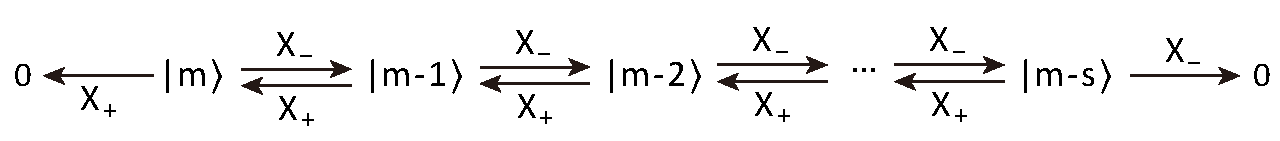
\includegraphics[width=0.8\textwidth ]{resources/figures/3_2_su2.pdf}
		\caption{How $X_+$ and $X_-$ acts in $H_0$.}
		\label{fig:su2} 
	\end{figure}
		
	
	Name the subspace spanned by $|m\rangle$ \dots $|m-s\rangle$ as $H_0$. This means $H_0$ is an invariant subspace of the ${\bf su}(2)$ Lie algebra. We want to prove that Lie algebra restricted on $H_0$ is irreducible. We only need to prove there is no proper non-vanishing invariant subspace of $H_0$. Let there be one, say $H'_0$. We can find an eigenstate of $X_3$ with largest eigenvalue $|\psi\rangle=c_{m-n}|m-n\rangle$ and $X_+|\psi\rangle=0$. This leads to $|\psi\rangle=c_m|m\rangle$. The we can use $X_-$ to recover all basis of in $H_0$. Thus $H'_0=H_0$, which is a contradiction. 
	
	Since the Lie algebras are Hermitian operators, $H_0^\perp$ is also an invariant subspace. Then we can repeat this whole procedure in $H_0^\perp$. In this way we can reduce the original representation into irreducible representations.

	Finally we calculate $C_{m-n}$	and get the explicit matrix form of ${\bf su}(2)$ Lie algebra restricted in $H_0$. It's easy to see $C^2_{m-1}=m$, and when $2\leq n\leq s$
	\begin{eqnarray}
		C_{m-n}^2&=&C_{m-n}^2\langle m-n|m-n\rangle\\
		&=&\langle m-n+1|X_+X_-|m-n+1\rangle\\
		&=&\langle m-n+1|X_-X_+|m-n+1\rangle+\langle m-n+1|[X_+,X_-]|m-n+1\rangle\\
		&=&\langle m-n+1|X_-|m-n+2\rangle \langle|m-n+2|X_+|m-n+1\rangle+ m-n+1\\
		&=&C_{m-n+1}^2+ m-n+1
	\end{eqnarray}
	
	Thus $C_{m-n}^2=m+(m-1)+\cdots+(m-n+1)=\frac 12 n(2m-n+1)$. From $C_{m-s}=0$ we have $s=2m+1$ which means $m$ is an integer or half-integer. Then the basis of $H_0$ is $|m\rangle$ \dots $|-m\rangle$, and
	\begin{eqnarray}
		\langle n'|X_-|n\rangle&=&C_{n'}\delta_{n',n-1}=\sqrt{\frac {(m-n+1)(m+n)}2}\delta_{n',n-1}\\
		\langle n'|X_+|n\rangle&=&C_{n}\delta_{n',n+1}=\sqrt{\frac {(m-n)(m+n+1)}2}\delta_{n',n+1}\\
		\langle n'|X_1|n\rangle&=&\frac 12\big(\sqrt{(m-n+1)(m+n)}\delta_{n',n-1}+\sqrt{(m-n)(m+n+1)}\delta_{n',n+1}\big)\\
		\langle n'|X_2|n\rangle&=&\frac i2\big(-\sqrt{(m-n+1)(m+n)}\delta_{n',n-1}+\sqrt{(m-n)(m+n+1)}\delta_{n',n+1}\big)\\
		\langle n'|X_3|n\rangle&=&n\delta_{n',n}
	\end{eqnarray}
	
	This is also called by physicists the spin-$m$ representation, expressed as $(m)$. For small $m$, its matrix form is
	\begin{enumerate}
		\item $m=0$, $X_i=0$
		\item $m=\frac 12$, $X_i=\frac{\sigma_i}2$
		\item $m=1$, 
			\begin{equation}
			X_1 =\frac 1{\sqrt 2}
			\left( \begin{array}{ccc}
			0&1&0\\
			1&0&1\\
			0&1&0  
			\end{array} \right)
			,\quad X_2 =\frac i{\sqrt 2}
			\left( \begin{array}{ccc}
			0&-1&0\\
			1&0&-1\\
			0&1&0  
			\end{array} \right)
			,\quad X_3 =
			\left( \begin{array}{ccc}
			1&0&0\\
			0&0&0\\
			0&0&-1  
			\end{array} \right)
			\end{equation}
		\item $m=\frac 32$, 
			\begin{equation}
			X_1 =
			\left( \begin{array}{cccc}
			0&\frac{\sqrt 3}2&0&0\\
			\frac{\sqrt 3}2&0&1&0\\
			0&1&0&\frac{\sqrt 3}2\\
			0&0&\frac{\sqrt 3}2&0  
			\end{array} \right)
			, X_2 =
			\left( \begin{array}{cccc}
			0&-\frac{\sqrt 3}2i&0&0\\
			\frac{\sqrt 3}2i&0&-i&0\\
			0&i&0&-\frac{\sqrt 3}2i\\
			0&0&\frac{\sqrt 3}2i&0
			\end{array} \right)
			, X_3 =
			\left( \begin{array}{cccc}
			\frac 32&0&0&0\\
			0&\frac 12&0&0\\
			0&0&\frac 12&0\\
			0&0&0&\frac 32  
			\end{array} \right)
			\end{equation}
	\end{enumerate}
	
	Then the original space $H$ can be reduced as in Fig \ref{fig:su2s}. If we define $D_m$ to be the dimension of eigenspace of $X_3$ with eigenvalue $m$. It's easy to see the recurrence of spin-$m$ representation is just $D_m-D_{m+1}$.
	
	\begin{figure}[htb]
		\centering  
		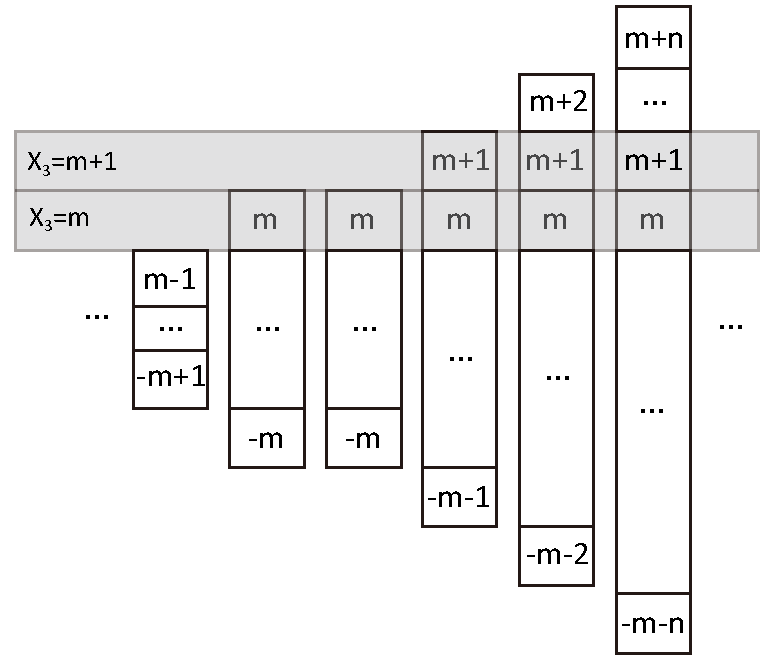
\includegraphics[width=280pt]{resources/figures/3_2_su2s.pdf}
		\caption{Reduction of $H$ into irreducible representations.}
		\label{fig:su2s} 
	\end{figure}
	\subsection{Tensor products}
	If we have a spin-$j$ and a spin-$j'$ representation of ${\bf su}(2)$ with representation space $H_1$ and $H_2$. In each space, basis of ${\bf su}(2)$ can be viewed as operators $X_i^{(1)}$ and $X_i^{(2)}$. We define operators acting in $H_1\otimes H_2$ as
	\begin{equation}
		X_i=X_i^{(1)}\otimes I^{(2)}+I^{(1)}\otimes X_i^{(2)}
	\end{equation}
	which is usually abbreviated as $X_i=X_i^{(1)}+X_i^{(2)}$.
	
	
		Test that $X_i$ satisfy ${\bf su}(2)$ algebra, and thus can be viewed as basis of ${\bf su}(2)$ algebra.
		
	Thus $X_i$ is naturally a ${\bf su}(2)$ representation. It's generally a reducible representation, and can be reduced to irreducible representations by a similar transformation, whose matrix elements are called the Clebsh-Gordan coefficients. It's easier for us to derive the recurrence of each irreducible representations by dimension counting.
	
	Since
	\begin{equation}
		X_3|m_1,m_2\rangle=(m+m')|m,m'\rangle
	\end{equation}
	$D_m$ we just defined is the number of solutions of
	\begin{equation}
		m_1+m_2=m,\ |m_1|\leq j,\ |m_2|\leq j'
	\end{equation}
	
	It's easy to see
	\begin{equation}
		D_m=\left\{\begin{array}{cc}
		0&|m|>|j+j'|\\
		j+j'-m+1&|j-j'|\leq|m|\leq|j+j'|\\
		2{\rm min}(j,j')+1&|m|<|j-j'|
		\end{array}\right.
	\end{equation}
	Thus
	\begin{equation}
		D_m-D_{m+1}=\left\{\begin{array}{cc}
		0&m>|j+j'|\\
		1&|j-j'|\leq m\leq|j+j'|\\
		0&0\leq m<|j-j'|
		\end{array}\right.
	\end{equation}
	That's to say, the direct product of spin-$j$ and a spin-$j'$ representation can be reduced into direct sum of spin-$|j-j'|$ \dots spin-$j+j'$ representation. It can also be expressed as 
	\begin{equation}
		(j)\otimes(j')=(|j-j'|)\oplus\cdots\oplus(j+j')
	\end{equation}
	This is called the Clebsh-Gordan series.
	
	
	
	
		Prove that for $\textbf{su}(2)$ algebra
		\begin{eqnarray}
		\Big(\frac 12\Big)^{\otimes 2N}&=&(0)^{g(0,N)}\oplus(1)^{g(1,N)}\oplus\cdots\oplus(N)^{g(N,N)}\\
		\Big(\frac 12\Big)^{\otimes(2N+1)}&=&\Big(\frac 12\Big)^{g(\frac 12,\frac {2N+1}2)}\oplus\Big(\frac 32\Big)^{g(\frac 32,\frac {2N+1}2)}\oplus\cdots\oplus\Big(\frac {2N+1}2\Big)^{g(\frac {2N+1}2,\frac {2N+1}2)}
		\end{eqnarray}
		where
		\begin{equation}
		g(a,b)=\left\{\begin{array}{ll}
		\left(\begin{array}{c}2b\\a+b\end{array}\right)-\left(\begin{array}{c}2b\\a+b+1\end{array}\right)&(a<b)\\
		1&(a=b)
		\end{array}\right.
		\end{equation}
		\textbf{Hint}: Count the dimension of the subspace with definite total $X^3$.

	
	
	
	
	
	
	
	
	
	
	
	
	
	
	
	
	\printindex
	\bibliographystyle{plain}%
	\bibliography{mybib}
\end{document}